\documentclass{classrep}
\usepackage[utf8]{inputenc}
\frenchspacing

\usepackage{graphicx}
\usepackage[usenames,dvipsnames]{color}
\usepackage[hidelinks]{hyperref}
\usepackage{float}

\usepackage{amsmath, amssymb, mathtools}

\usepackage{fancyhdr, lastpage}
\pagestyle{fancyplain}
\fancyhf{}
\renewcommand{\headrulewidth}{0pt}
\cfoot{\thepage\ / \pageref*{LastPage}}

\renewcommand{\refname}{Bibliografia}

% csharp cmd
\newcommand{\Csharp}{%
  {\settoheight{\dimen0}{C}C\kern-.05em \resizebox{!}{\dimen0}{\raisebox{\depth}{\# }}}}

\studycycle{Informatyka stosowana, studia dzienne, II st.}
\coursesemester{I}

\coursename{Obliczenia ewolucyjne}
\courseyear{2019/2020}

\courseteacher{dr inż. Łukasz Chomątek}
\coursegroup{środa, 14:00}

\author{%
  \\
  \studentinfo[234067@edu.p.lodz.pl]{Bartosz Jurczewski}{234067}\\
  \studentinfo[234106@edu.p.lodz.pl]{Karol Podlewski}{234106}%
}

\title{Zadanie 2: Optymalizacja wielokryterialna funkcji}

\begin{document}
\maketitle
\thispagestyle{fancyplain}

\clearpage

\section{Cel}

Celem zadania była optymalizacja wielokryterialna funkcji wielu zmiennych na zadanym przedziale. Należało wykorzystać algorytmy do rozwiązywania problemów, dla których znany jest front Pareto.


\section{Opis implementacji}

Zadanie zostało zrealizowane w języku Python, w wersji 3.7.5, z wykorzystaniem bibliotek: Matplotlib, NumPy, \href{https://github.com/Project-Platypus/Platypus}{Platypus-Opt (algorytmy genetyczne)}  oraz \href{https://pymoo.org}{Pymoo (ewaluacja)}.


\section{Wprowadzenie}

\subsection{Algorytmy genetyczne}
W przygotowanym rozwiązaniu porównane ze sobą zostały trzy algorytmy przeznaczone do optymalizacji wielokryterialnej funkcji: NSGA-II, SPEA-II oraz PESA-II . 

\begin{itemize}
    \item \textbf{NSGA-II} - jest to obecnie używana, poprawiona wersja algorytmu NSGA (ang. \textit{Non-dominated Sorting Genetic Algorithm}). Kroki algorytmu:
    \begin{enumerate}
        \item Losowe utworzenie populacji $P(0)$. $t = 0$. 
        \item Przez mutację i krzyżowanie na zbiorze $P(t)$ zostaje utworzony zbiór $Q(t)$.
        \item Zbiory $P(t)$ oraz $Q(t)$ zostają połączone w jeden zbiór $R(t)$. Dla każdego rozwiązania ze zbioru $R(t)$ zostaje wyliczona siła w zależności od poziomu w którym jest ona niezdominowana. Następnie wartości te są sortowane.
        \item Zbiór $R(t)$ zostaje zmniejszony do wielkości populacji przez usunięcie najsłabszych wartości - algorytm stara się usunąć takie rozwiązania, wokół których znajduje się wiele innych najsłabszych rozwiązań.
        \item Jeżeli osiągnięto wymaganą liczbę epok $t$, algorytm zostaje przerwany, zbiór $P(t+1)$ jest jego wynikiem.
        \item $t = t + 1$. Jeżeli nie, należy wrócić do punktu 2.
    \end{enumerate}
    \cite{CleverAlgs}\cite{NSGA}
    \item \textbf{SPEA-II} - jest to najpopularniejsze rozszerzenie algorytmu SPEA (ang. \textit{Strength Pareto Evolutionary Algorithm}). Kroki algorytmu:
    \begin{enumerate}
        \item Losowe utworzenie populacji $P(0)$ oraz utworzenie pustego zbioru rozwiązań niezdominowanych $A(0)$. $t = 0$. 
        \item Wyliczenie dopasowania dla każdego ze zbiorów ($P(t)$ oraz $A(t)$).
        \item Skopiowanie wszystkich niezdominowanych rozwiązań z obu zbiorów do nowego zbioru rozwiązań niezdominowanych $A(t+1)$. Jeżeli zbiór przekracza maksymalną wielkość ustaloną przed rozpoczęciem działania algorytmu, zostaje zmniejszony z wykorzystaniem algorytmu klastrowania. Jeżeli zbiór jest za mały, zostaje wypełniony rozwiązaniami zdominowanymi o najlepszym dopasowaniu.
        \item Jeżeli osiągnięto wymaganą liczbę epok $t$, algorytm zostaje przerwany, zbiór $A(t+1)$ jest jego wynikiem.
        \item Jeżeli nie, zbiór $A(t+1)$ zostaje poddany selekcji turniejowej w celu utworzenia zbioru o wielkości populacji, który, będąc poddanym mutacji oraz krzyżowaniu, tworzy zbiór $P(t+1)$.
        \item $t = t + 1$. Należy przejść do kroku 2.
    \end{enumerate}
    Algorytm SPEA-II względem pierwowzoru poprawił obliczanie dopasowania, metody zmniejszania oraz wypełniania zbioru $A(t+1)$ oraz zmienił zbiór, który jest poddany mutacji \cite{CleverAlgs}\cite{SPEA2_1}\cite{SPEA2_2}.
    \item \textbf{PESA-II} - jest to druga wersja algorytmu PESA (ang. \textit{Pareto Envelope-based Selection Algorithm}). Kroki algorytmu:
    \begin{enumerate}
        \item Losowe utworzenie populacji $P(0)$ oraz utworzenie pustego zbioru rozwiązań niezdominowanych $A(0)$. $t = 0$. 
        \item Skopiowanie wszystkich niezdominowanych rozwiązań ze zbioru $P(t)$ do zbioru $A(t)$.
        \item Jeżeli osiągnięto wymaganą liczbę epok $t$, algorytm zostaje przerwany. Zbiór $A(t)$ jest jego wynikiem.
        \item Jeżeli nie, przez mutację i krzyżowanie na zbiorze $A(t)$, zostaje utworzony zbiór $P(t+1)$.
        \item $t = t + 1$. Należy przejść do kroku 2.
    \end{enumerate}
    \cite{PESA}
\end{itemize}


\subsection{Problemy testowe}

Przygotowane rozwiązanie obsługuje trzy problemy testowe: \textbf{ZDT1}, \textbf{ZDT2} i \textbf{ZDT3}. Dla każdego z nich rozwiązania są tym lepsze, im bliżej frontu Pareto leżą.

\begin{figure}[H]
    \centering
    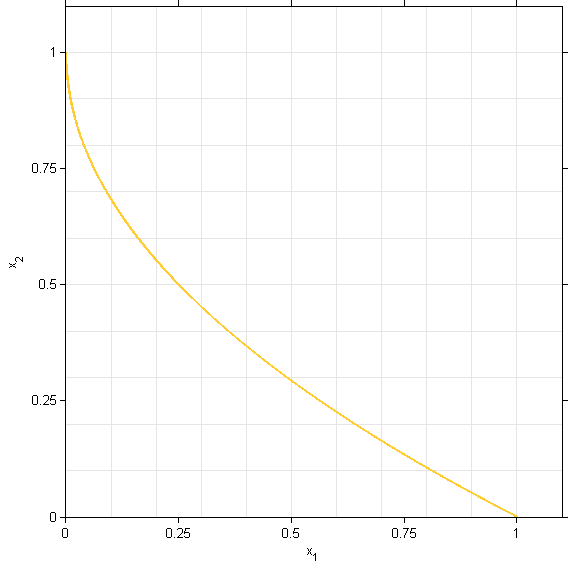
\includegraphics[width=0.6\textwidth]{img2/zdt1.png}
    \caption{Problem ZDT1 \url{http://people.ee.ethz.ch/~sop/download/supplementary/testproblems/zdt1/index.php}}
\end{figure}

\begin{figure}[H]
    \centering
    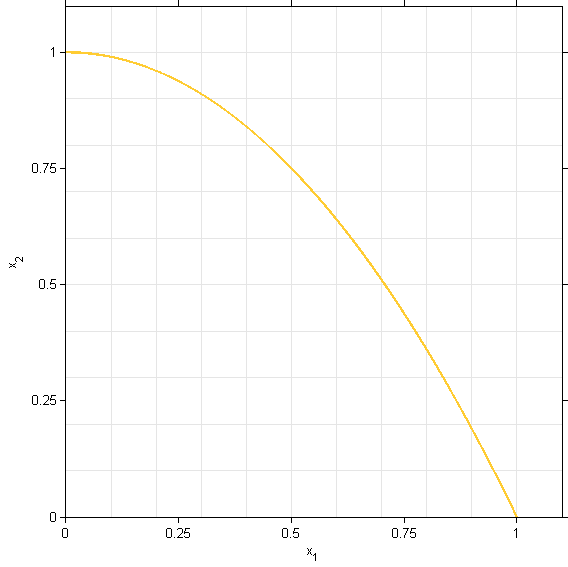
\includegraphics[width=0.6\textwidth]{img2/zdt2.png}
    \caption{Problem ZDT2 \url{http://people.ee.ethz.ch/~sop/download/supplementary/testproblems/zdt2/index.php}}
\end{figure}

\begin{figure}[H]
    \centering
    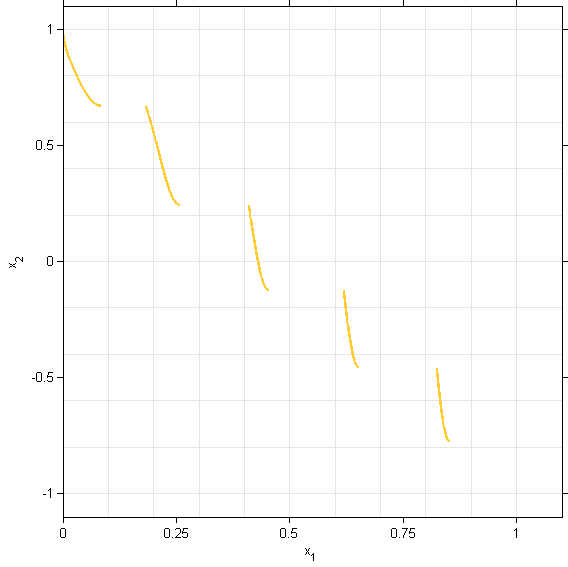
\includegraphics[width=0.6\textwidth]{img2/zdt3.png}
    \caption{Problem ZDT3 \url{http://people.ee.ethz.ch/~sop/download/supplementary/testproblems/zdt3/index.php}}
\end{figure}


\subsection{Miary oceny algorytmów}

Przygotowane rozwiązanie ocenia działanie algorytmu przy użyciu dwóch miar:

\begin{enumerate}
    \item \textbf{Generational Distance (GD)} - miara oblicza średnią odległość euklidesową każdego rozwiązania do najbliższego punktu na froncie Pareto. Im mniejszy wynik, tym algorytm znalazł lepsze rozwiązanie.
    \item \textbf{Hypervolume (HV)} - miara oblicza pole powierzchni między niezdominowanymi rozwiązaniami, a wybranym punktem referencyjnym (w przypadku prezentowanego rozwiązania jest to punkt x=1, y=5). Im wyższy wynik, tym algorytm znalazł lepsze rozwiązanie.
    \begin{figure}[H]
        \centering
        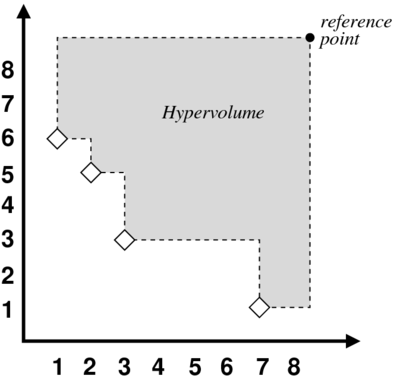
\includegraphics[width=0.7\textwidth]{img2/hypervolume.png}
        \caption{Prezentacja miary Hypervolume dla 2 wymiarowej przestrzeni \newline \url{http://lopez-ibanez.eu/hypervolume}}
    \end{figure}
    
\end{enumerate}


%%%%%%%%%%%%%%%%%%%%%%%%%%%%%%%%%%%%%%%%%%%%  WYNIKI

\newpage
\section{Wyniki}

Dla każdego algorytmu została porównana wielkość populacji oraz prawdopodobieństw operatorów. W przypadku algorytmów SPEA-II oraz PESA-II został porównany także dodatkowy atrybut, charakterystyczny dla danego algorytmu, z uwzględnieniem najlepszych uzyskanych wyników dla wcześniejszych testów.

\subsection{Algorytm NSGA-II}

\subsubsection{Problem testowy ZDT1}

\begin{table}[H]
\centering
\caption{Wyniki algorytmu NSGA-II dla problemu ZDT1}
\label{tab:NSGAII_ZDT1}
\begin{tabular}{|ccc|c|c|}
\hline
\textbf{Generacje} & \textbf{Populacja} & \textbf{Prawdo.} & \textbf{GD} & \textbf{HV} \\ \hline
1000 & 50 & 0,25 & 1,353 & 2,789 \\ \hline
\textbf{1000} & \textbf{50} & \textbf{0,5} & \textbf{1,344} & \textbf{2,939} \\ \hline
\textbf{1000} & \textbf{50} & \textbf{0,75} & \textbf{1,442} & \textbf{3,008} \\ \hline
1000 & 100 & 0,25 & 2,033 & 2,337 \\ \hline
1000 & 100 & 0,5 & 1,786 & 2,523 \\ \hline
1000 & 100 & 0,75 & 1,66 & 2,669 \\ \hline
1000 & 200 & 0,25 & 2,168 & 2,183 \\ \hline
1000 & 200 & 0,5 & 2,191 & 2,098 \\ \hline
1000 & 200 & 0,75 & 2,273 & 2,074 \\ \hline
\textbf{10000} & \textbf{50} & \textbf{0,25} & \textbf{0,05} & \textbf{4,589} \\ \hline
10000 & 50 & 0,5 & 0,158 & 4,438 \\ \hline
10000 & 50 & 0,75 & 0,228 & 4,359 \\ \hline
10000 & 100 & 0,25 & 0,159 & 4,44 \\ \hline
10000 & 100 & 0,5 & 0,235 & 4,338 \\ \hline
10000 & 100 & 0,75 & 0,251 & 4,292 \\ \hline
10000 & 200 & 0,25 & 0,511 & 3,96 \\ \hline
10000 & 200 & 0,5 & 0,471 & 4,025 \\ \hline
10000 & 200 & 0,75 & 0,601 & 3,921 \\ \hline
100000 & 50 & 0,25 & 0,005 & 4,656 \\ \hline
100000 & 50 & 0,5 & 0,028 & 4,622 \\ \hline
100000 & 50 & 0,75 & 0,074 & 4,557 \\ \hline
100000 & 100 & 0,25 & 0,005 & 4,661 \\ \hline
100000 & 100 & 0,5 & 0,033 & 4,616 \\ \hline
100000 & 100 & 0,75 & 0,087 & 4,538 \\ \hline
\textbf{100000} & \textbf{200} & \textbf{0,25} & \textbf{0,005} & \textbf{4,663} \\ \hline
100000 & 200 & 0,5 & 0,042 & 4,604 \\ \hline
100000 & 200 & 0,75 & 0,112 & 4,508 \\ \hline
\end{tabular}
\end{table}

\begin{figure}[H]
    \centering
    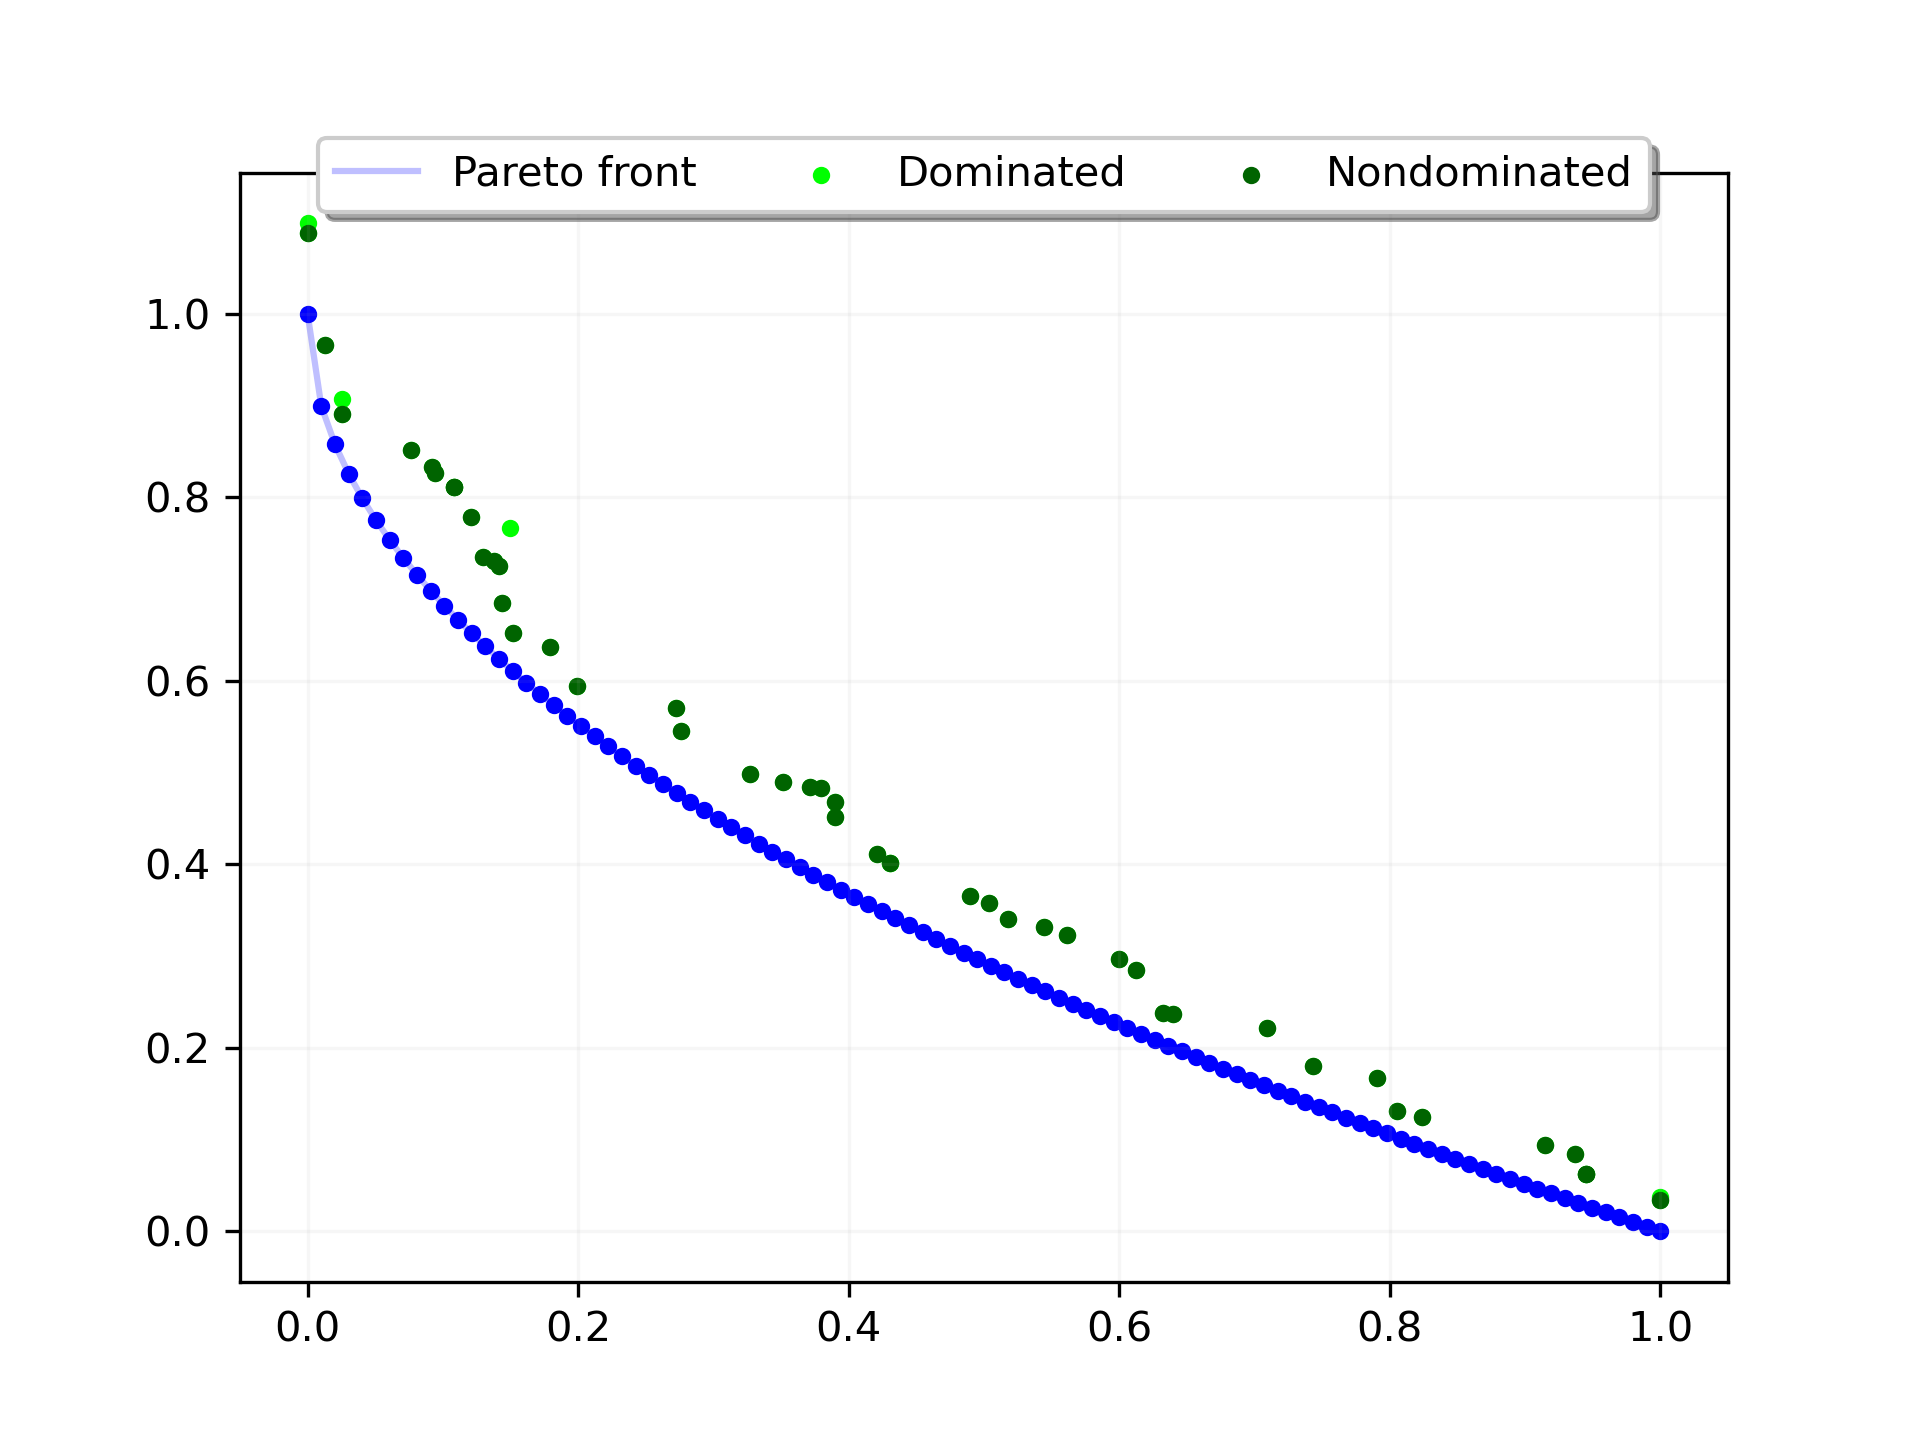
\includegraphics[width=0.9\textwidth]{img2/NSGAII_ZDT1_g10000_p50_r0,25.png}
    \caption{Algorytm NSGA-II, problem ZDT1, \newline generacje - 10 000, populacja - 50, prawdopodobieństwo - 0,25}
\end{figure}

\begin{figure}[H]
    \centering
    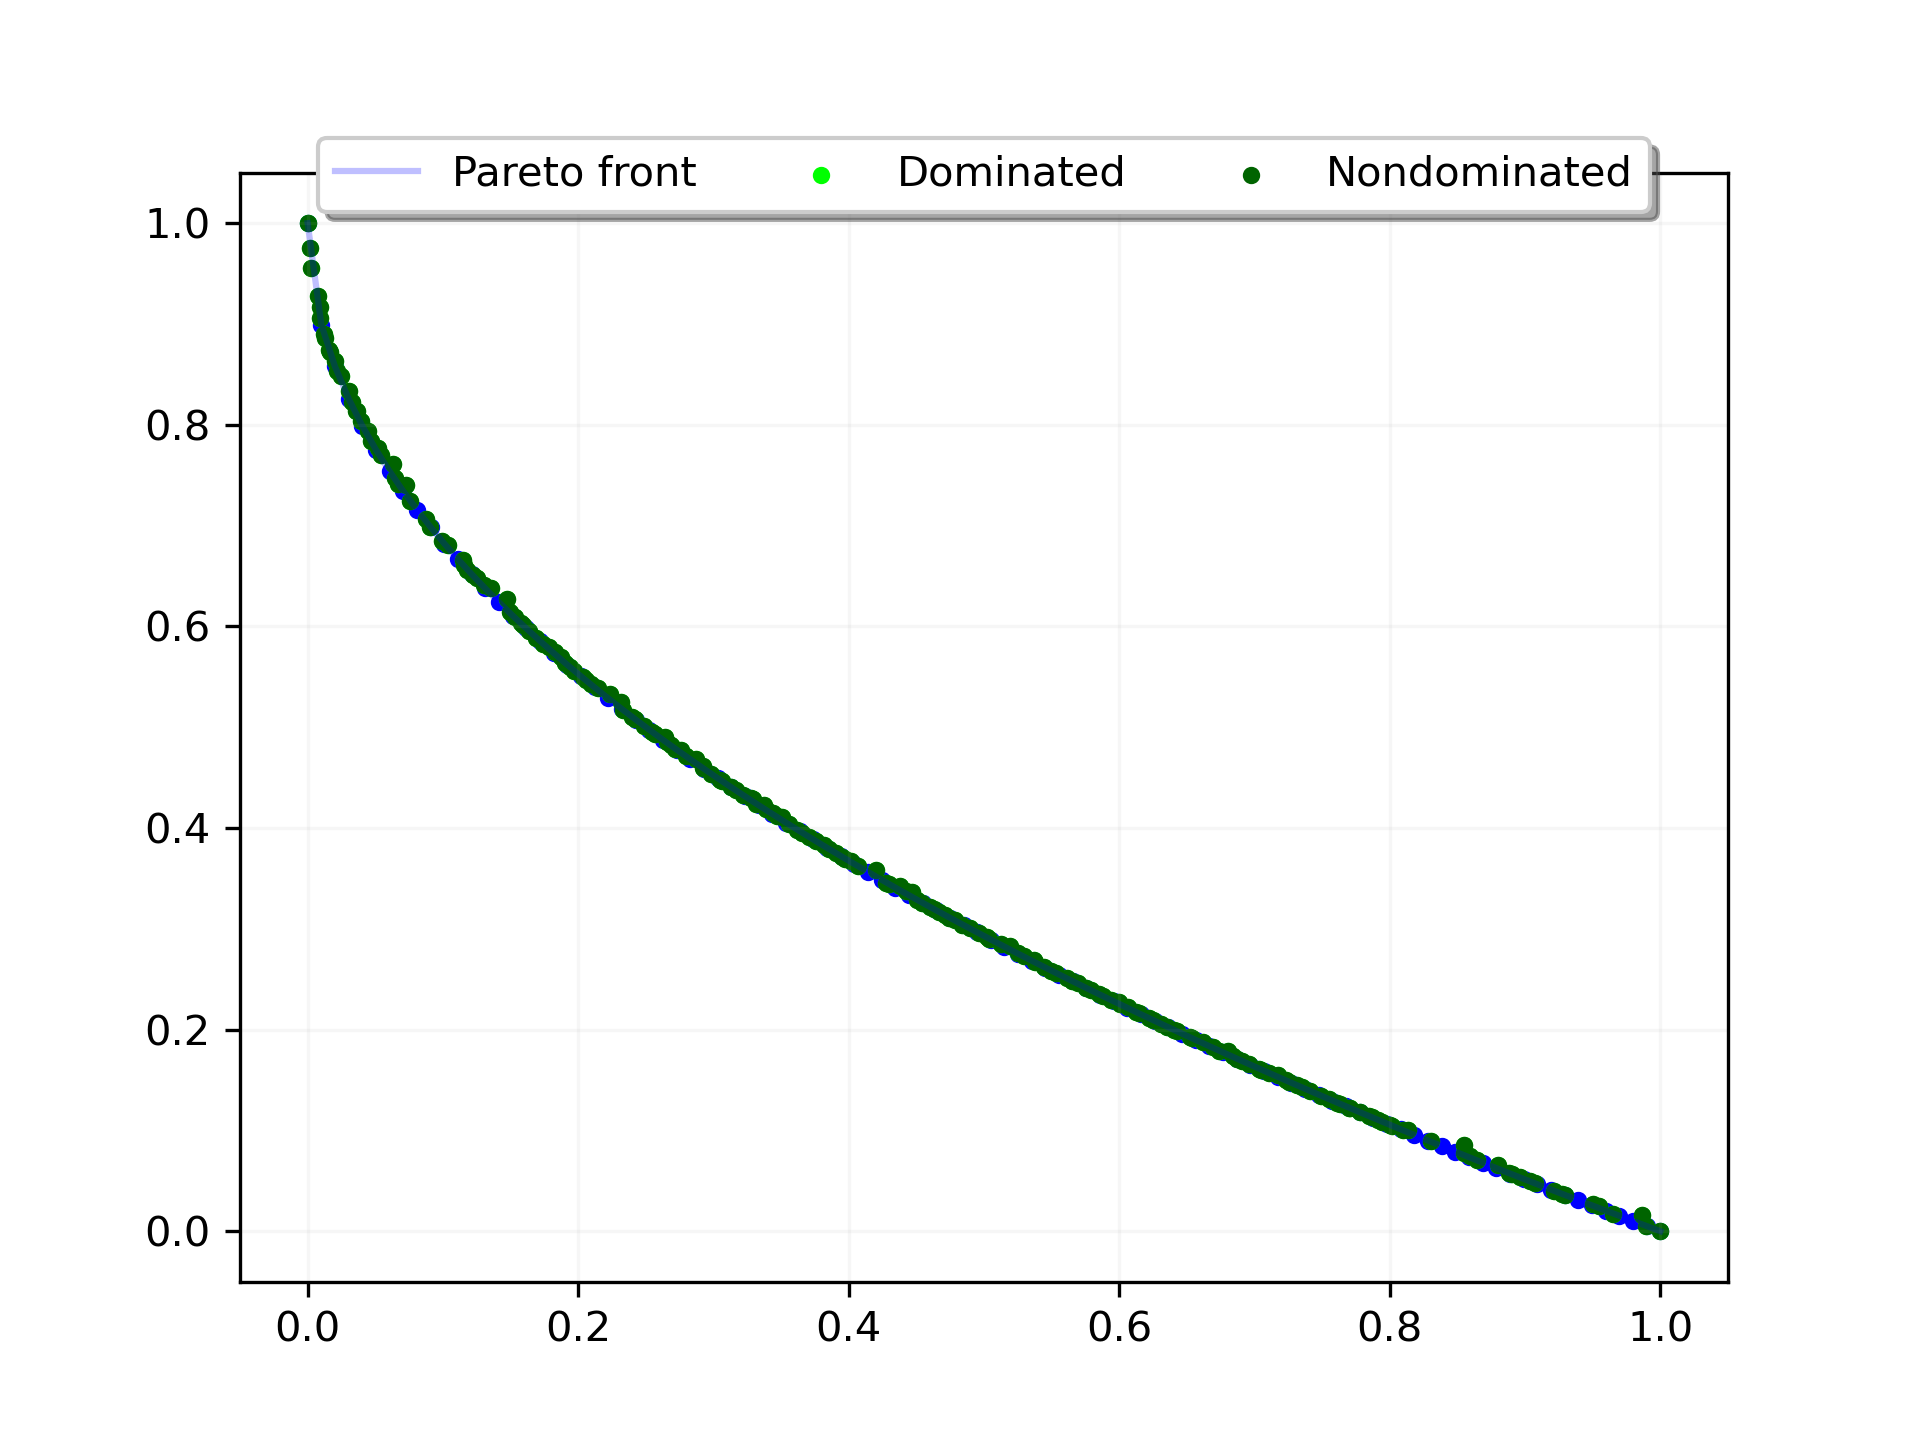
\includegraphics[width=0.9\textwidth]{img2/NSGAII_ZDT1_g100000_p200_r0,25.png}
    \caption{Algorytm NSGA-II, problem ZDT1, \newline generacje - 100 000, populacja - 200, prawdopodobieństwo - 0,25}
\end{figure}

\subsubsection{Problem testowy ZDT2}

\begin{table}[H]
\centering
\caption{Wyniki algorytmu NSGA-II dla problemu ZDT2}
\label{tab:NSGAII_ZDT2}
\begin{tabular}{|ccc|c|c|}
\hline
\textbf{Generacje} & \textbf{Populacja} & \textbf{Prawdo.} & \textbf{GD} & \textbf{HV} \\ \hline
1000 & 50 & 0,25 & 2,339 & 1,689 \\ \hline
1000 & 50 & 0,5 & 2,01 & 2,065 \\ \hline
\textbf{1000} & \textbf{50} & \textbf{0,75} & \textbf{1,662} & \textbf{2,424} \\ \hline
1000 & 100 & 0,25 & 2,813 & 1,194 \\ \hline
1000 & 100 & 0,5 & 2,761 & 1,295 \\ \hline
1000 & 100 & 0,75 & 2,07 & 1,923 \\ \hline
1000 & 200 & 0,25 & 2,949 & 1,086 \\ \hline
1000 & 200 & 0,5 & 3,001 & 1,022 \\ \hline
1000 & 200 & 0,75 & 2,66 & 1,258 \\ \hline
\textbf{10000} & \textbf{50} & \textbf{0,25} & \textbf{0,047} & \textbf{4,246} \\ \hline
10000 & 50 & 0,5 & 0,243 & 3,982 \\ \hline
10000 & 50 & 0,75 & 0,314 & 3,885 \\ \hline
10000 & 100 & 0,25 & 0,119 & 4,15 \\ \hline
10000 & 100 & 0,5 & 0,356 & 3,844 \\ \hline
10000 & 100 & 0,75 & 0,402 & 3,811 \\ \hline
10000 & 200 & 0,25 & 0,321 & 3,679 \\ \hline
10000 & 200 & 0,5 & 0,742 & 3,513 \\ \hline
10000 & 200 & 0,75 & 0,576 & 3,555 \\ \hline
100000 & 50 & 0,25 & 0,004 & 4,323 \\ \hline
100000 & 50 & 0,5 & 0,032 & 4,282 \\ \hline
100000 & 50 & 0,75 & 0,128 & 4,146 \\ \hline
100000 & 100 & 0,25 & 0,004 & 4,328 \\ \hline
100000 & 100 & 0,5 & 0,049 & 4,256 \\ \hline
100000 & 100 & 0,75 & 0,144 & 4,132 \\ \hline
\textbf{100000} & \textbf{200} & \textbf{0,25} & \textbf{0,004} & \textbf{4,329} \\ \hline
100000 & 200 & 0,5 & 0,063 & 4,233 \\ \hline
100000 & 200 & 0,75 & 0,175 & 4,074 \\ \hline
\end{tabular}
\end{table}

\begin{figure}[H]
    \centering
    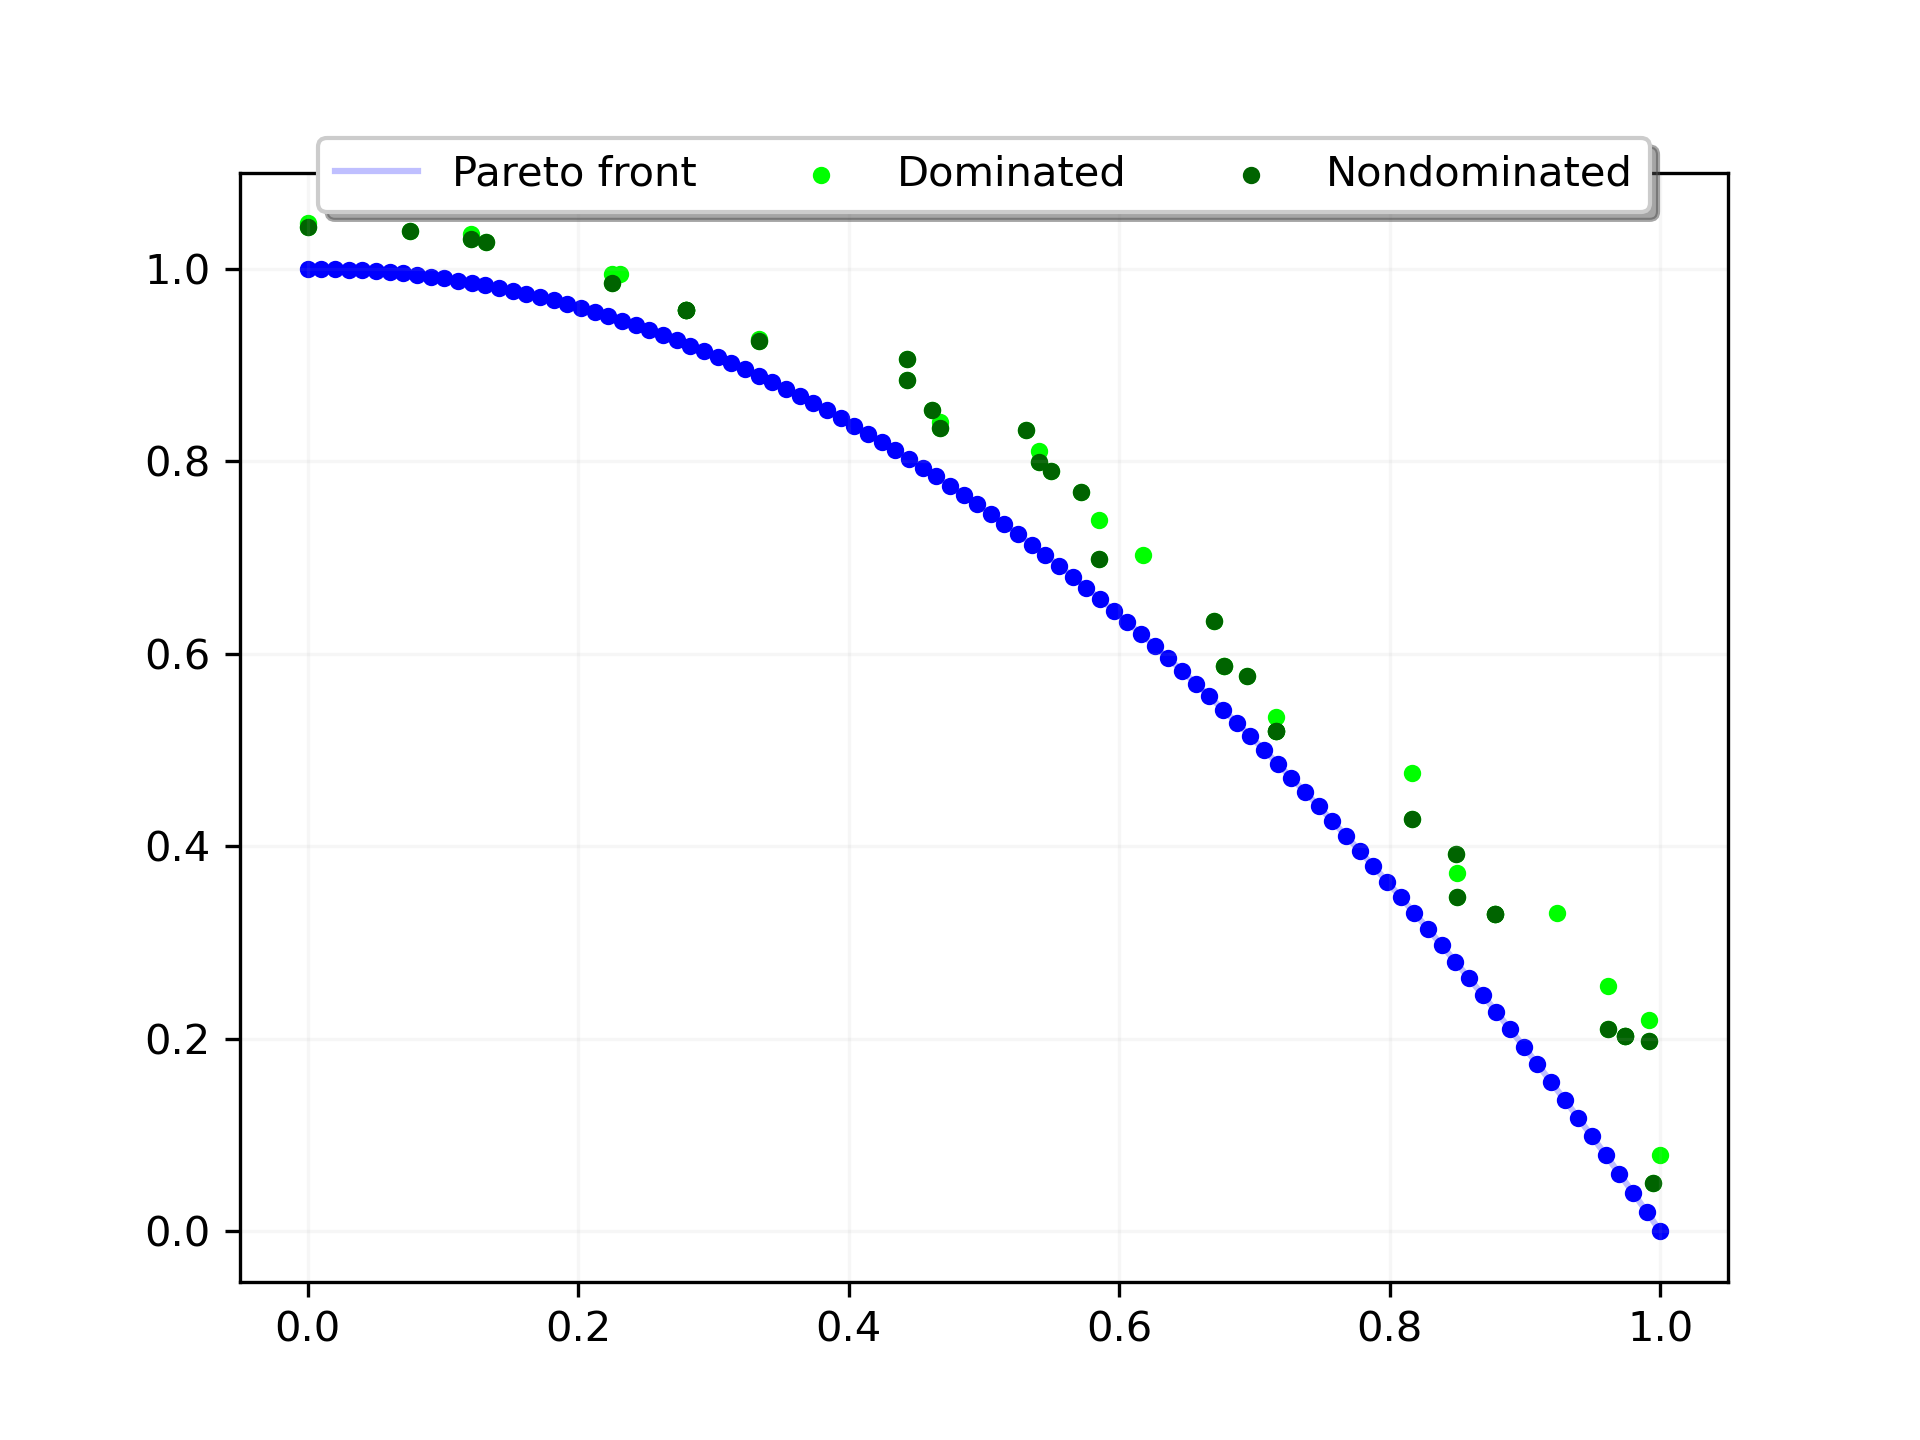
\includegraphics[width=0.9\textwidth]{img2/NSGAII_ZDT2_g10000_p50_r0,25.png}
    \caption{Algorytm NSGA-II, problem ZDT2, \newline generacje - 10 000, populacja - 50, prawdopodobieństwo - 0,25}
\end{figure}

\begin{figure}[H]
    \centering
    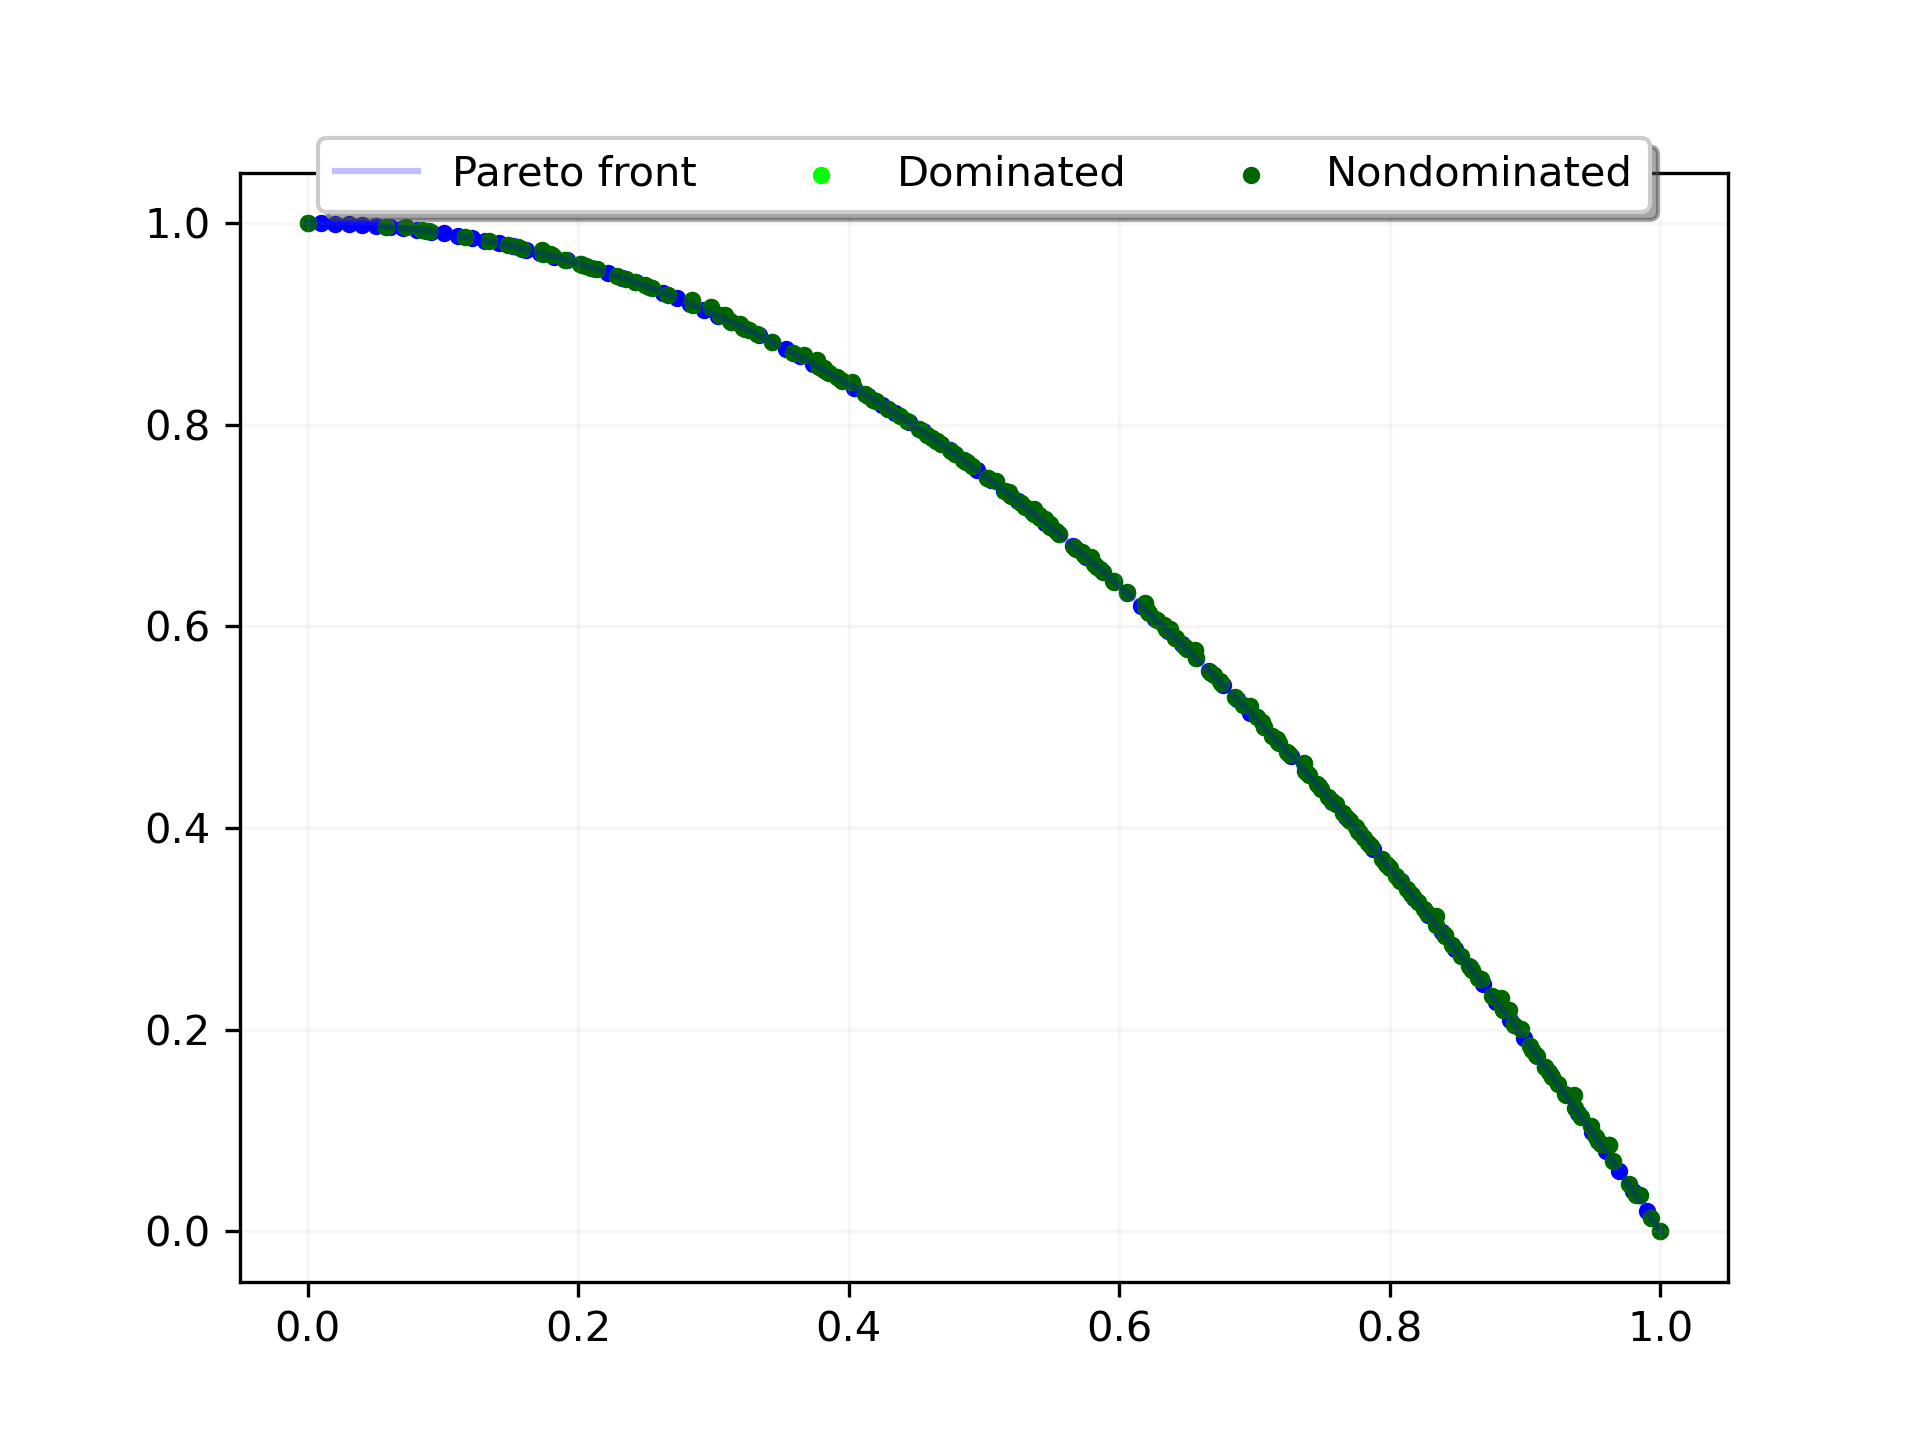
\includegraphics[width=0.9\textwidth]{img2/NSGAII_ZDT2_g100000_p200_r0,25.png}
    \caption{Algorytm NSGA-II, problem ZDT2, \newline generacje - 100 000, populacja - 200, prawdopodobieństwo - 0,25}
\end{figure}

\subsubsection{Problem testowy ZDT3}

\begin{table}[H]
\centering
\caption{Wyniki algorytmu NSGA-II dla problemu ZDT3}
\label{tab:NSGAII_ZDT3}
\begin{tabular}{|ccc|c|c|}
\hline
\textbf{Generacje} & \textbf{Populacja} & \textbf{Prawdo.} & \textbf{GD} & \textbf{HV} \\ \hline
1000 & 50 & 0,25 & 1,529 & 2,929 \\ \hline
1000 & 50 & 0,5 & 1,507 & 2,947 \\ \hline
\textbf{1000} & \textbf{50} & \textbf{0,75} & \textbf{1,422} & \textbf{3,013} \\ \hline
1000 & 100 & 0,25 & 1,695 & 2,508 \\ \hline
1000 & 100 & 0,5 & 1,725 & 2,884 \\ \hline
1000 & 100 & 0,75 & 1,724 & 2,716 \\ \hline
1000 & 200 & 0,25 & 2,002 & 2,509 \\ \hline
1000 & 200 & 0,5 & 1,875 & 2,5 \\ \hline
1000 & 200 & 0,75 & 2,095 & 2,564 \\ \hline
\textbf{10000} & \textbf{50} & \textbf{0,25} & \textbf{0,022} & \textbf{4,937} \\ \hline
10000 & 50 & 0,5 & 0,087 & 4,773 \\ \hline
10000 & 50 & 0,75 & 0,144 & 4,682 \\ \hline
10000 & 100 & 0,25 & 0,085 & 4,784 \\ \hline
10000 & 100 & 0,5 & 0,148 & 4,683 \\ \hline
10000 & 100 & 0,75 & 0,234 & 4,546 \\ \hline
10000 & 200 & 0,25 & 0,518 & 4,198 \\ \hline
10000 & 200 & 0,5 & 0,374 & 4,311 \\ \hline
10000 & 200 & 0,75 & 0,492 & 4,178 \\ \hline
100000 & 50 & 0,25 & 0,006 & 5,038 \\ \hline
100000 & 50 & 0,5 & 0,013 & 4,997 \\ \hline
100000 & 50 & 0,75 & 0,039 & 4,905 \\ \hline
\textbf{100000} & \textbf{100} & \textbf{0,25} & \textbf{0,006} & \textbf{5,04} \\ \hline
100000 & 100 & 0,5 & 0,016 & 4,983 \\ \hline
100000 & 100 & 0,75 & 0,059 & 4,881 \\ \hline
100000 & 200 & 0,25 & 0,006 & 5,039 \\ \hline
100000 & 200 & 0,5 & 0,021 & 4,966 \\ \hline
100000 & 200 & 0,75 & 0,044 & 4,883 \\ \hline
\end{tabular}
\end{table}

\begin{figure}[H]
    \centering
    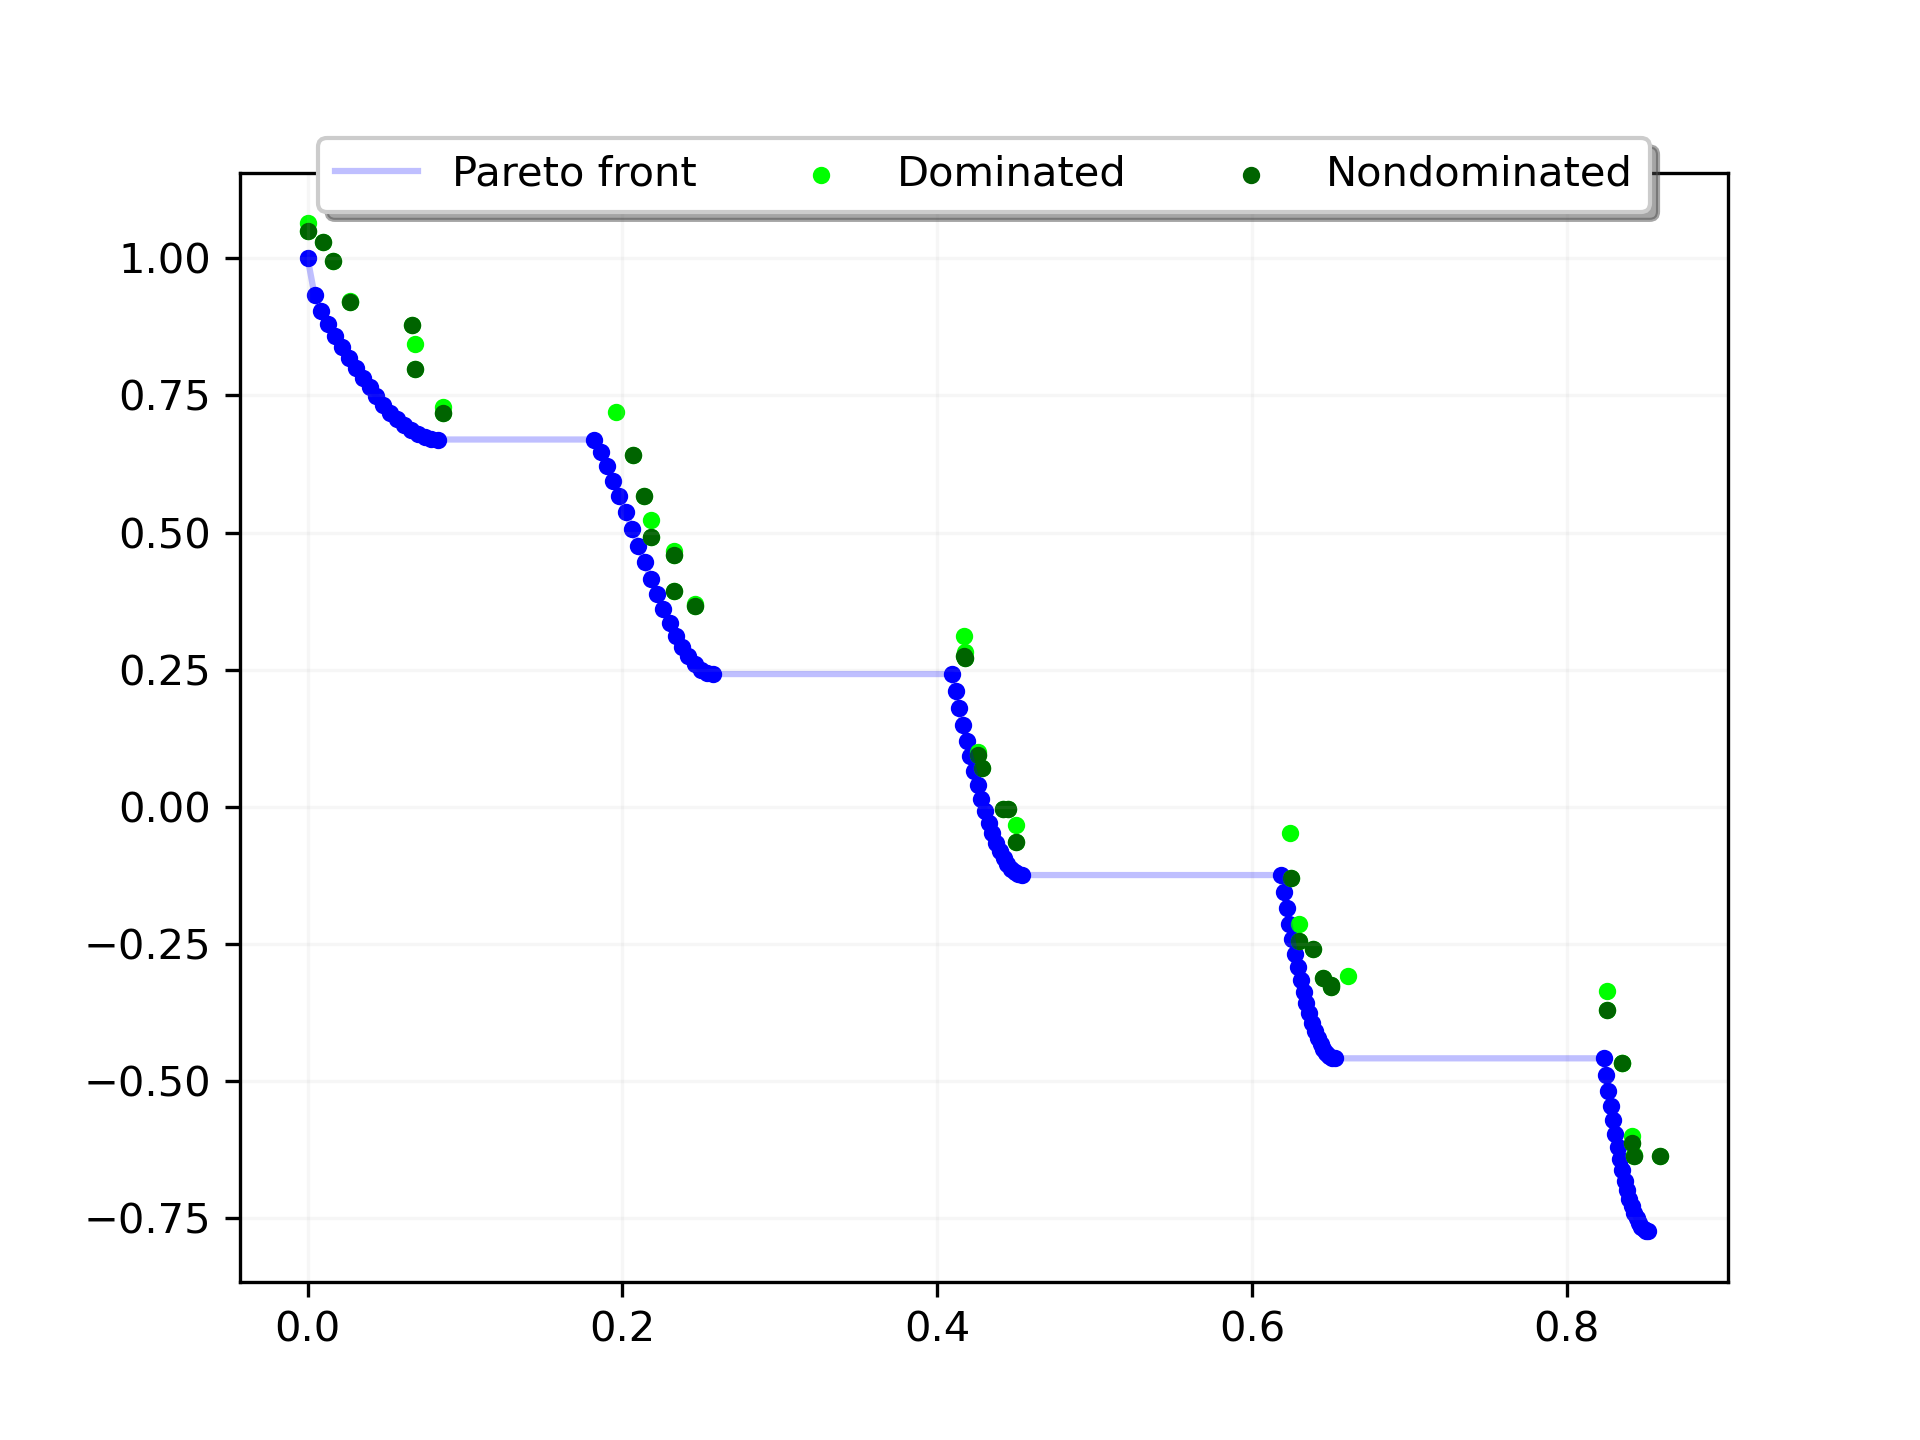
\includegraphics[width=0.9\textwidth]{img2/NSGAII_ZDT3_g10000_p50_r0,25.png}
    \caption{Algorytm NSGA-II, problem ZDT3, \newline generacje - 10 000, populacja - 50, prawdopodobieństwo - 0,25}
\end{figure}

\begin{figure}[H]
    \centering
    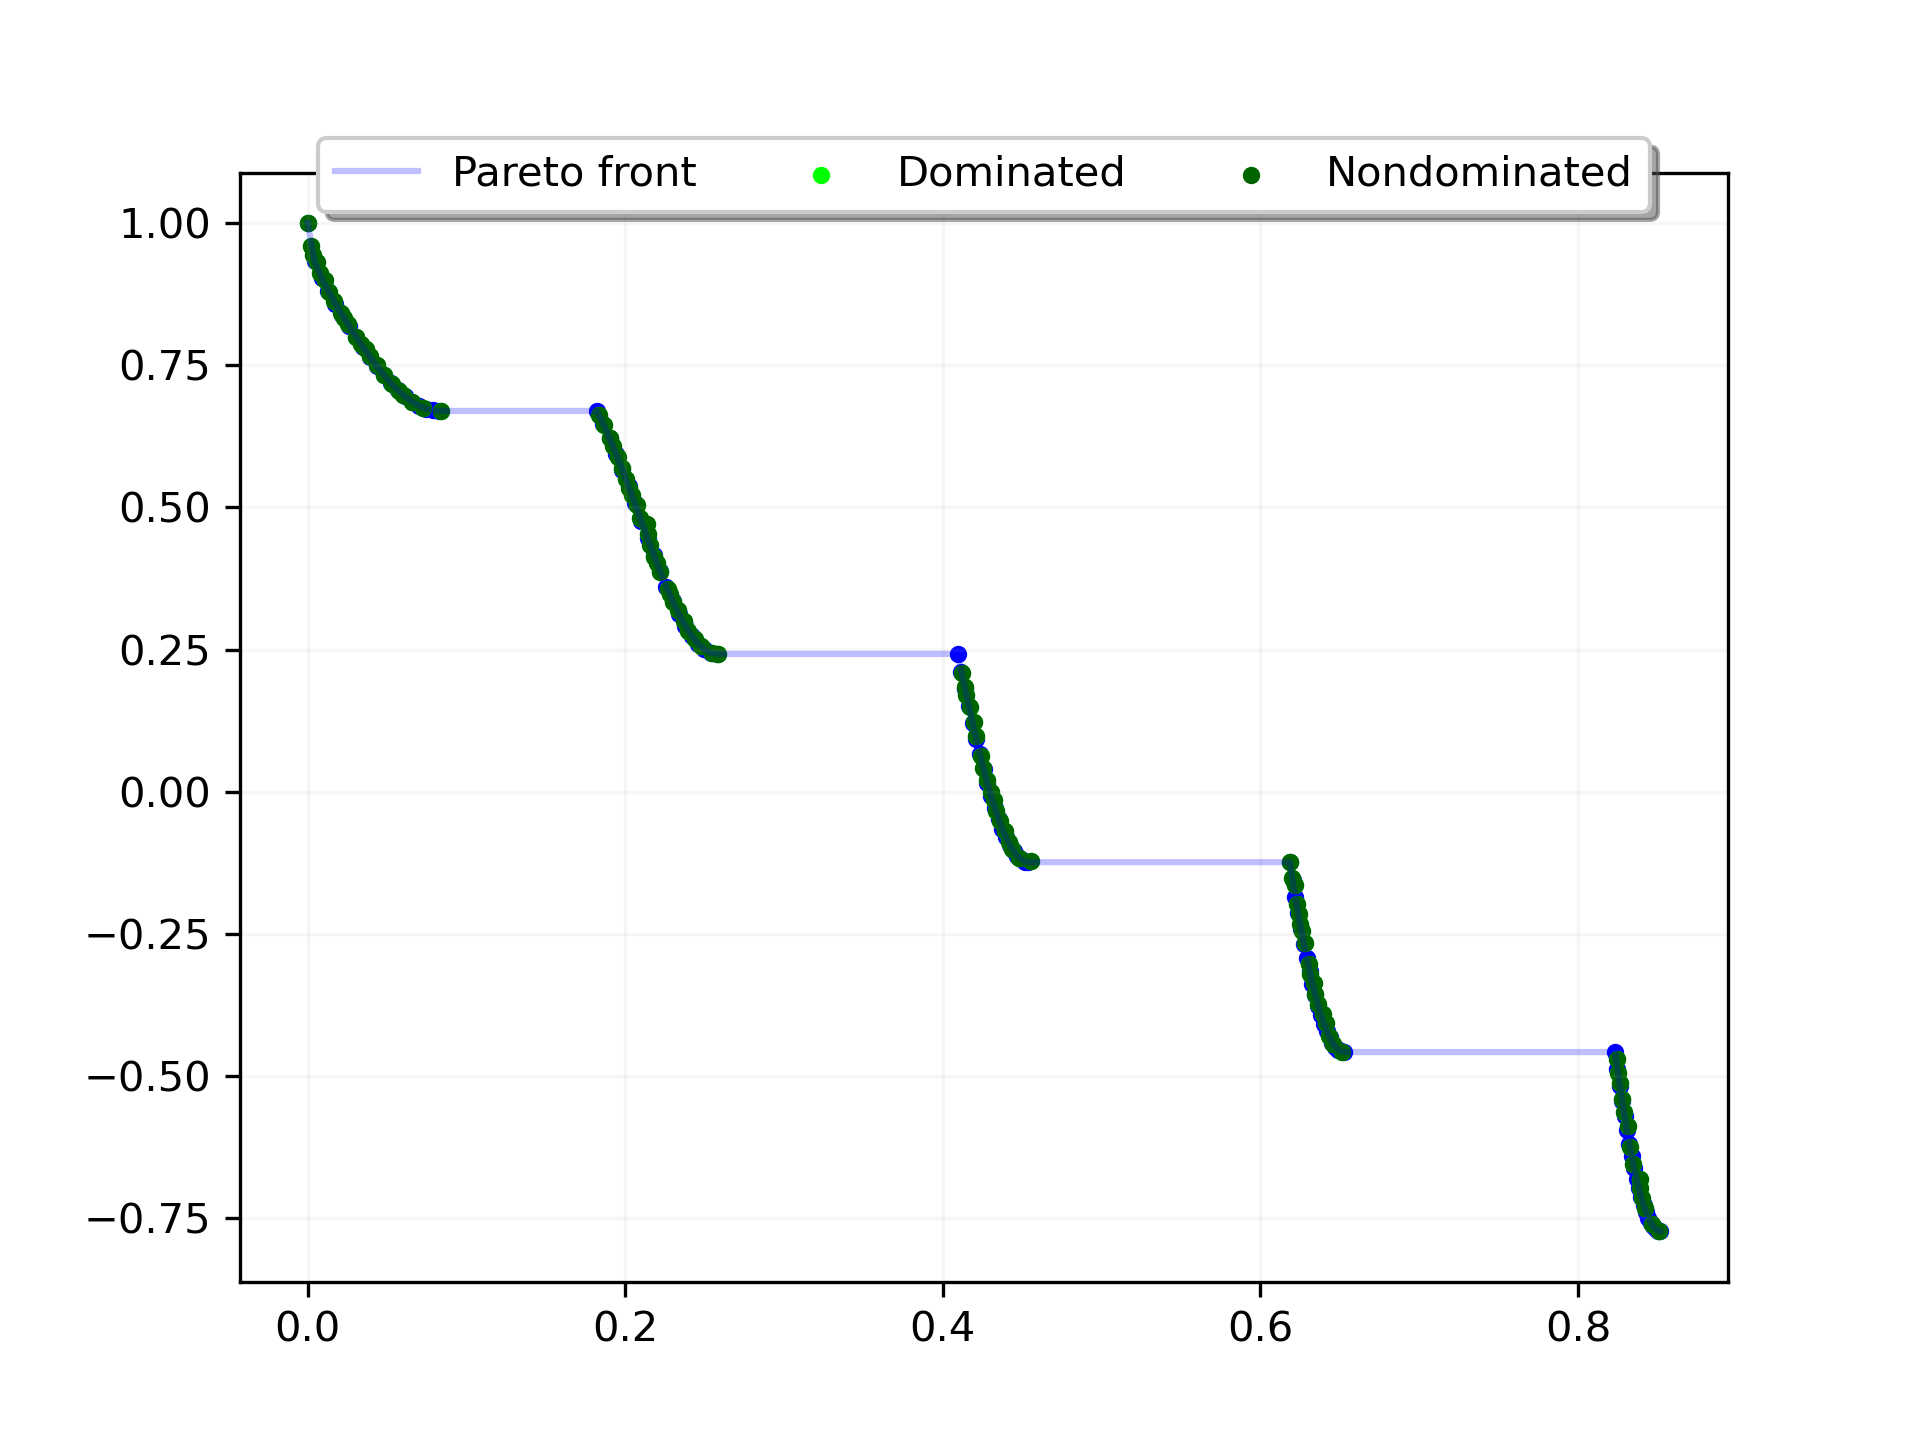
\includegraphics[width=0.9\textwidth]{img2/NSGAII_ZDT3_g100000_p100_r0,25.png}
    \caption{Algorytm NSGA-II, problem ZDT3, \newline generacje - 100 000, populacja - 100, prawdopodobieństwo - 0,25}
\end{figure}

\subsection{Algorytm SPEA-II}

Ze względu na bardzo długi czas działania algorytmu dla 100 000 generacji oraz 200 epok, wyniki przy tej konfiguracji nie zostały uwzględnione w tabelach.

\subsubsection{Problem testowy ZDT1}

\begin{table}[H]
\centering
\caption{Wyniki algorytmu SPEA-II dla problemu ZDT1}
\label{tab:SPEAII_ZDT1}
\begin{tabular}{|ccc|c|c|}
\hline
\textbf{Generacje} & \textbf{Populacja} & \textbf{Prawdo.} & \textbf{GD} & \textbf{HV} \\ \hline
1000 & 50 & 0,25 & 2,337 & 2,143 \\ \hline
1000 & 50 & 0,5 & 1,811 & 2,404 \\ \hline
\textbf{1000} & \textbf{50} & \textbf{0,75} & \textbf{1,796} & \textbf{2,51} \\ \hline
1000 & 100 & 0,25 & 2,543 & 1,906 \\ \hline
1000 & 100 & 0,5 & 2,436 & 1,994 \\ \hline
1000 & 100 & 0,75 & 2,349 & 2,017 \\ \hline
1000 & 200 & 0,25 & 2,54 & 1,826 \\ \hline
1000 & 200 & 0,5 & 2,599 & 1,716 \\ \hline
1000 & 200 & 0,75 & 2,229 & 2,005 \\ \hline
\textbf{10000} & \textbf{50} & \textbf{0,25} & \textbf{0,164} & \textbf{4,418} \\ \hline
10000 & 50 & 0,5 & 0,244 & 4,328 \\ \hline
10000 & 50 & 0,75 & 0,276 & 4,285 \\ \hline
10000 & 100 & 0,25 & 0,485 & 4,022 \\ \hline
10000 & 100 & 0,5 & 0,474 & 4,002 \\ \hline
10000 & 100 & 0,75 & 0,477 & 3,958 \\ \hline
10000 & 200 & 0,25 & 1,178 & 3,174 \\ \hline
10000 & 200 & 0,5 & 0,922 & 3,43 \\ \hline
10000 & 200 & 0,75 & 0,987 & 3,325 \\ \hline
100000 & 50 & 0,25 & 0,005 & 4,656 \\ \hline
100000 & 50 & 0,5 & 0,028 & 4,62 \\ \hline
100000 & 50 & 0,75 & 0,084 & 4,539 \\ \hline
\textbf{100000} & \textbf{100} & \textbf{0,25} & \textbf{0,005} & \textbf{4,661} \\ \hline
100000 & 100 & 0,5 & 0,049 & 4,595 \\ \hline
100000 & 100 & 0,75 & 0,106 & 4,515 \\ \hline
\end{tabular}
\end{table}

\begin{figure}[H]
    \centering
    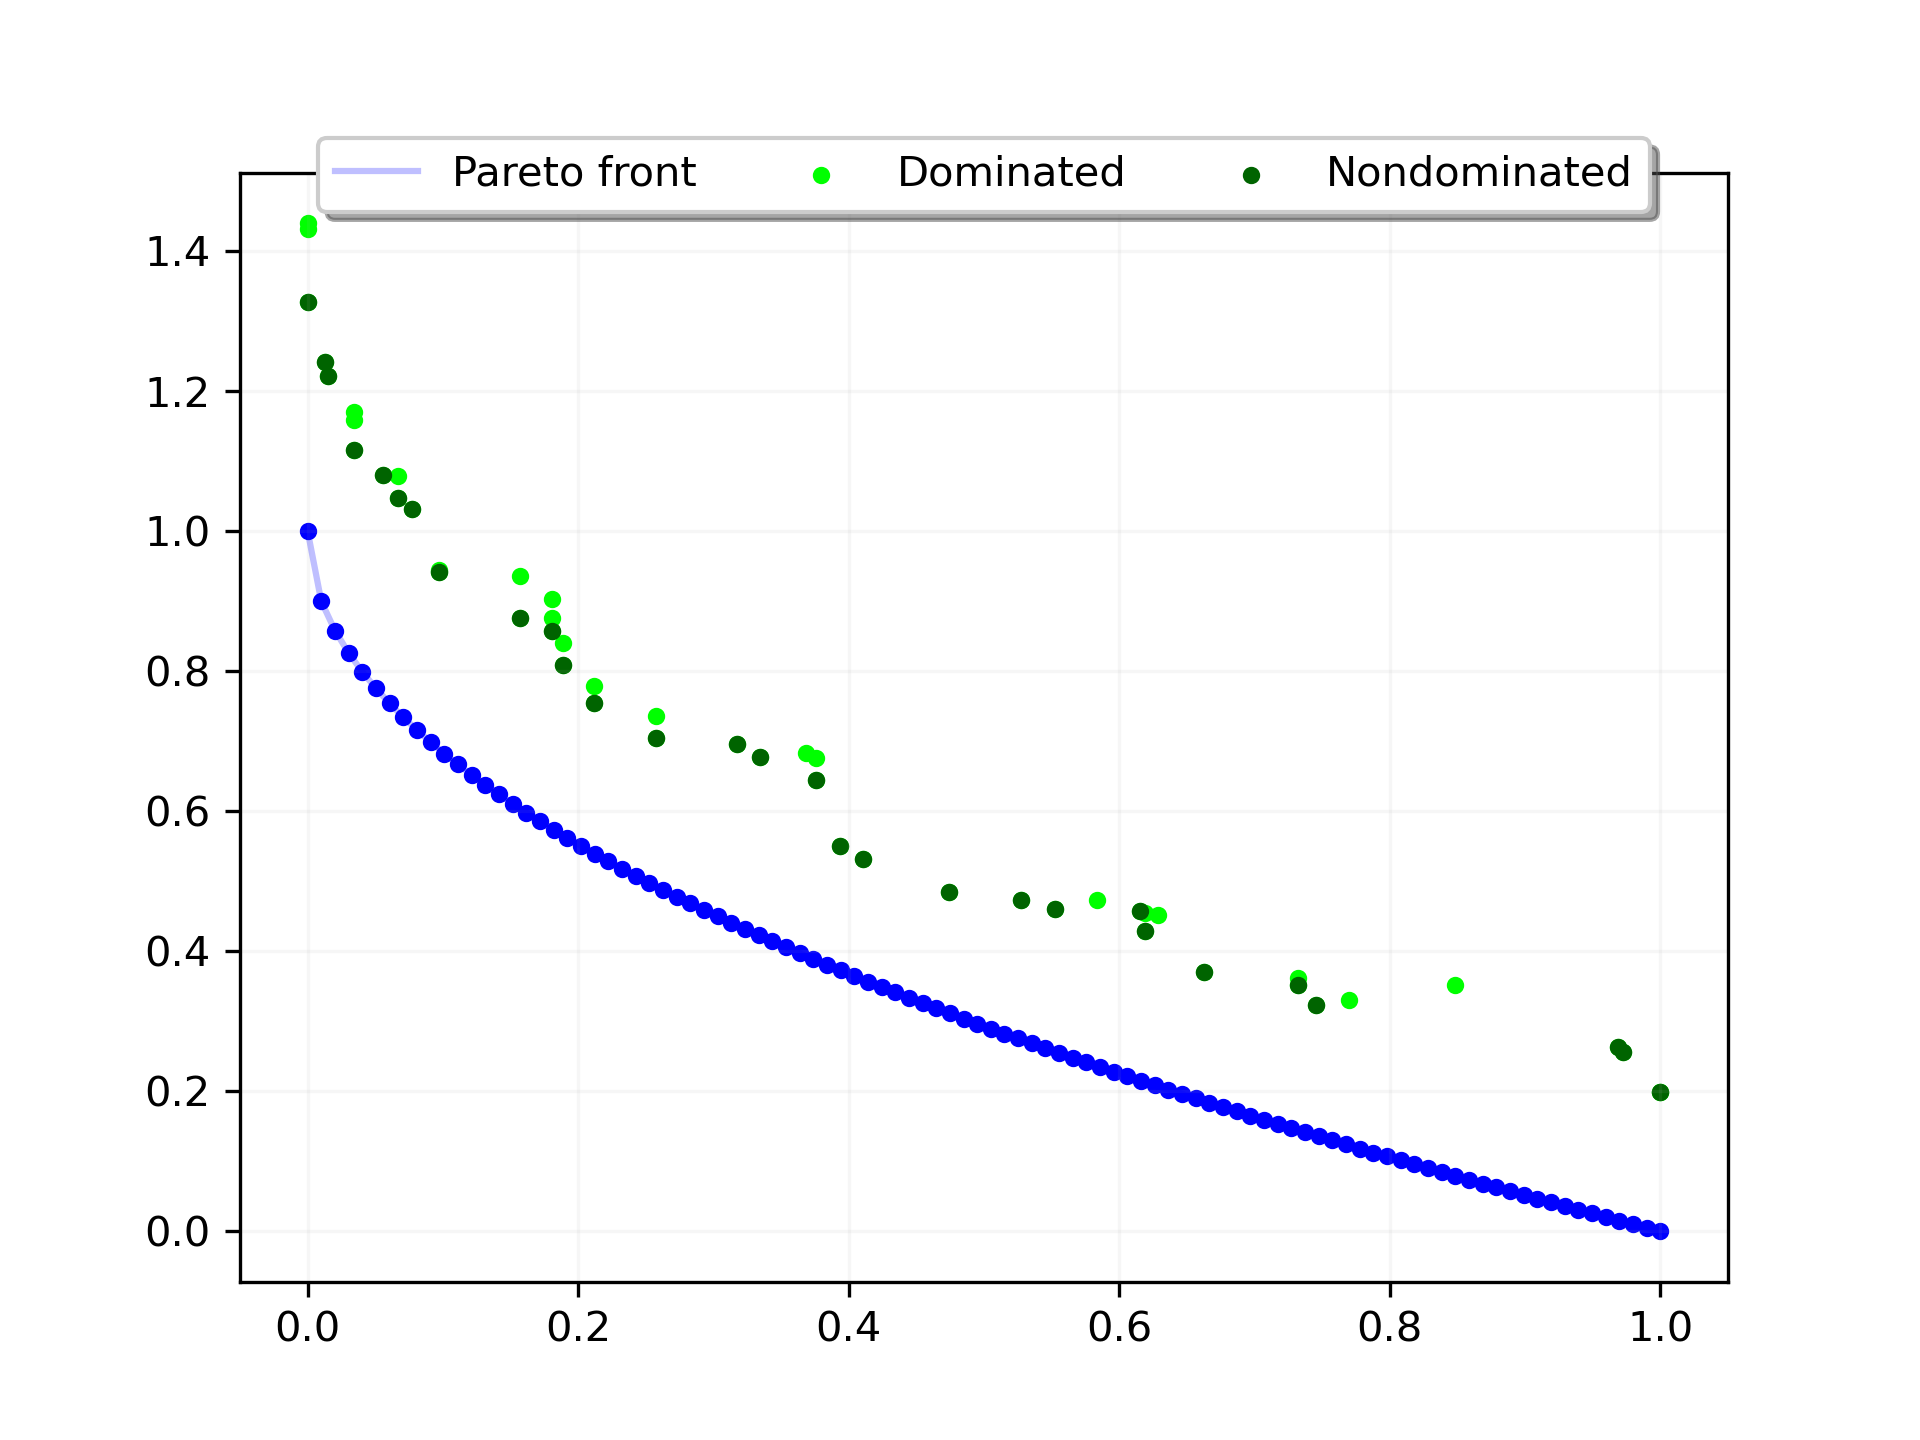
\includegraphics[width=0.9\textwidth]{img2/SPEAII_ZDT1_g10000_p50_r0,25.png}
    \caption{Algorytm SPEA-II, problem ZDT1, \newline generacje - 10 000, populacja - 50, prawdopodobieństwo - 0,25}
\end{figure}

\begin{figure}[H]
    \centering
    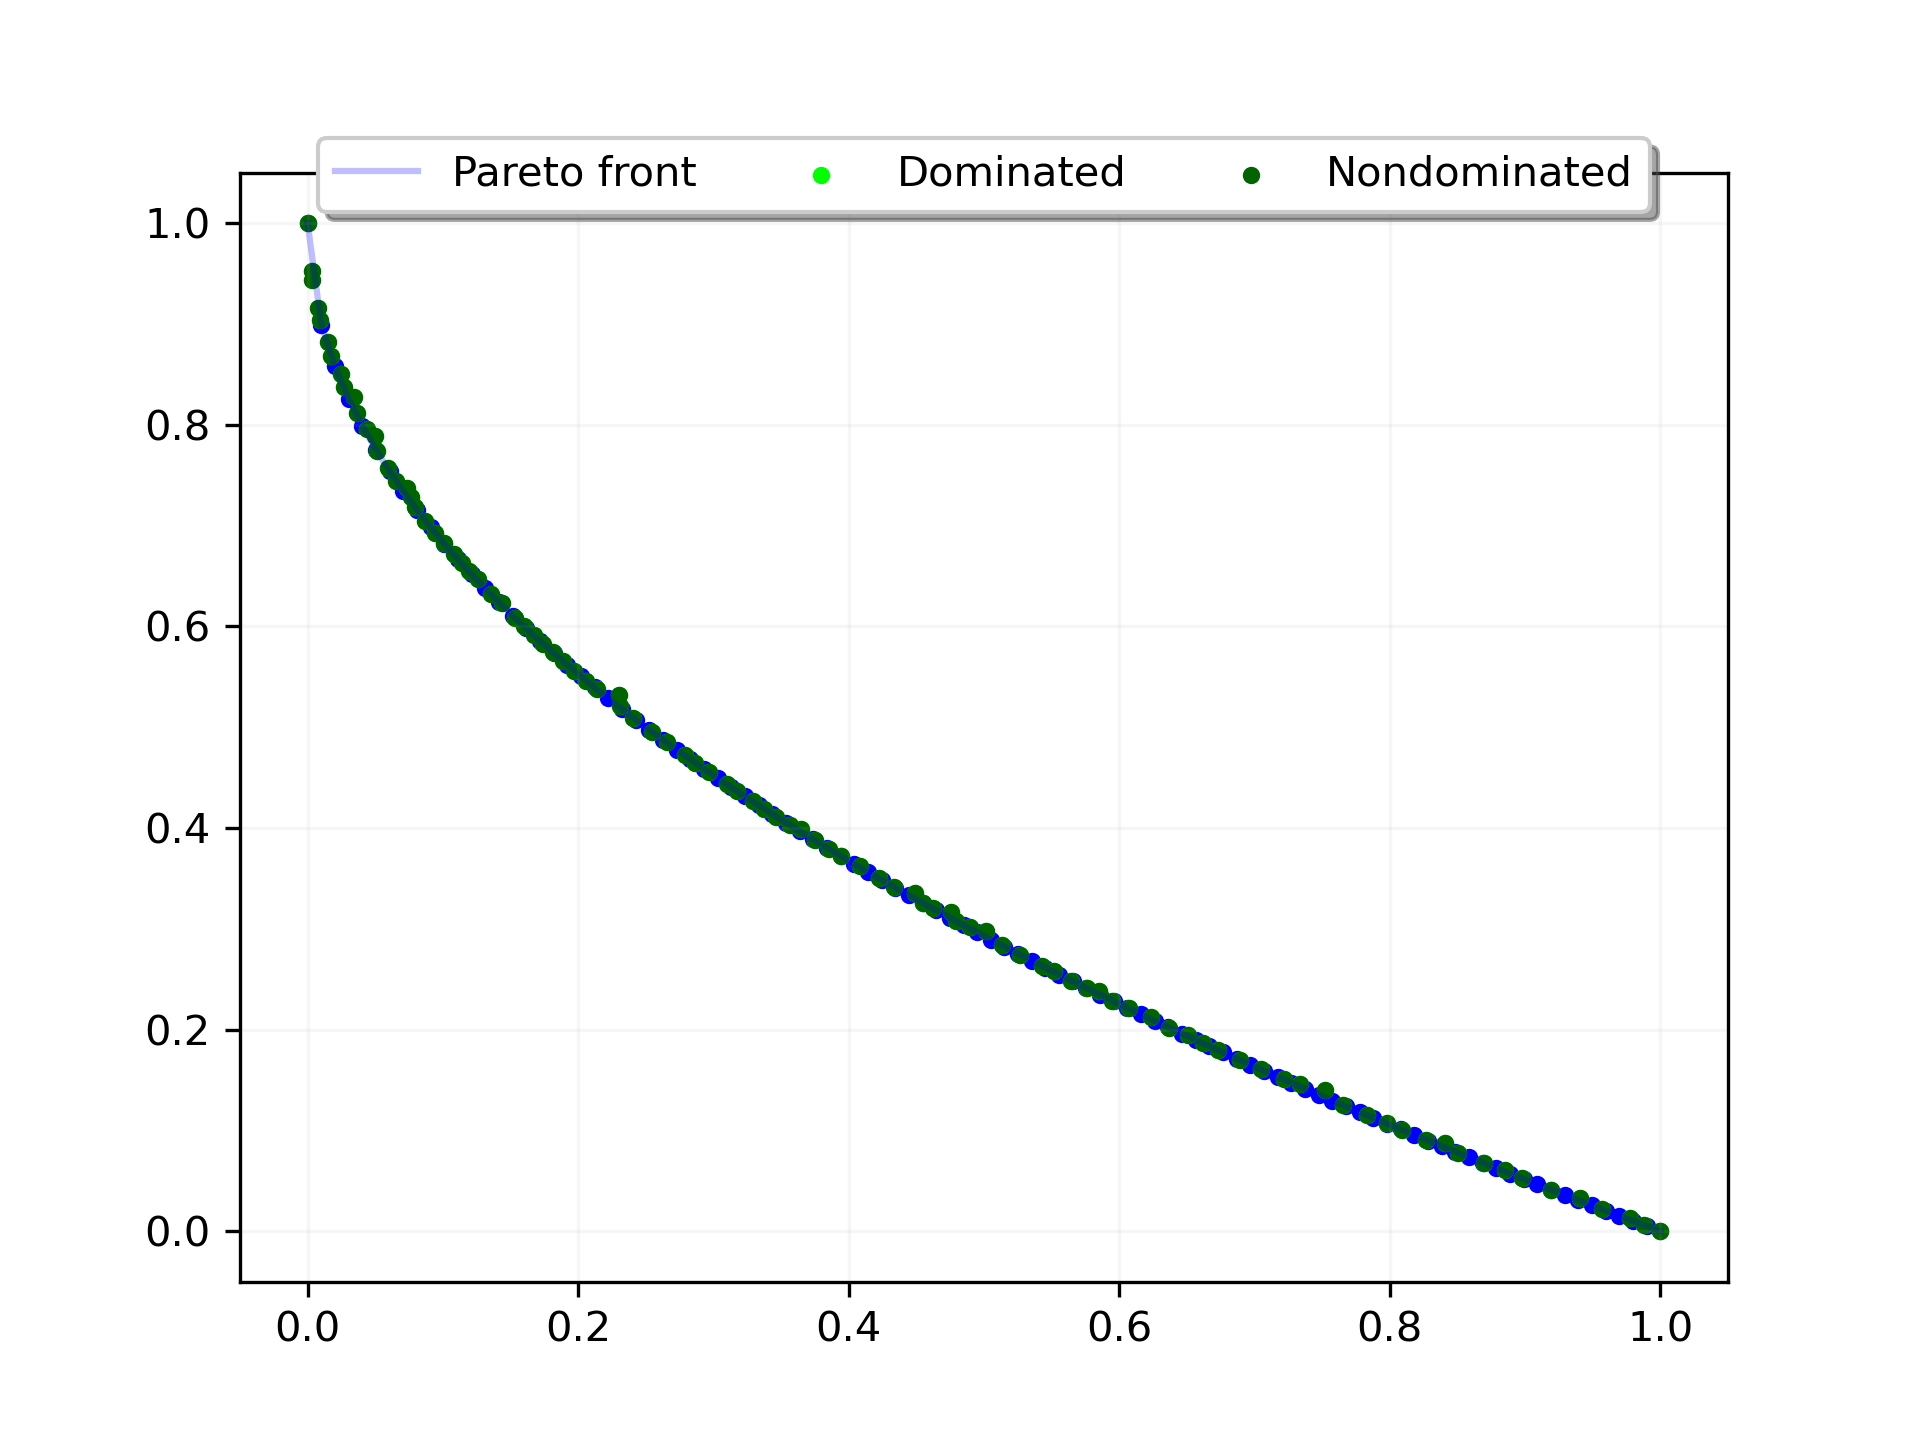
\includegraphics[width=0.9\textwidth]{img2/SPEAII_ZDT1_g100000_p100_r0,25.png}
    \caption{Algorytm SPEA-II, problem ZDT1, \newline generacje - 100 000, populacja - 100, prawdopodobieństwo - 0,25}
\end{figure}

\subsubsection{Problem testowy ZDT2}

\begin{table}[H]
\centering
\caption{Wyniki algorytmu SPEA-II dla problemu ZDT2}
\label{tab:SPEAII_ZDT2}
\begin{tabular}{|ccc|c|c|}
\hline
\textbf{Generacje} & \textbf{Populacja} & \textbf{Prawdo.} & \textbf{GD} & \textbf{HV} \\ \hline
1000 & 50 & 0,25 & 3,186 & 0,939 \\ \hline
\textbf{1000} & \textbf{50} & \textbf{0,5} & \textbf{2,609} & \textbf{1,442} \\ \hline
1000 & 50 & 0,75 & 2,808 & 1,259 \\ \hline
1000 & 100 & 0,25 & 3,38 & 0,663 \\ \hline
1000 & 100 & 0,5 & 3,43 & 0,623 \\ \hline
1000 & 100 & 0,75 & 3,259 & 0,915 \\ \hline
1000 & 200 & 0,25 & 3,539 & 0,752 \\ \hline
1000 & 200 & 0,5 & 3,386 & 0,693 \\ \hline
1000 & 200 & 0,75 & 3,435 & 0,806 \\ \hline
\textbf{10000} & \textbf{50} & \textbf{0,25} & \textbf{0,205} & \textbf{4,033} \\ \hline
10000 & 50 & 0,5 & 0,407 & 3,77 \\ \hline
10000 & 50 & 0,75 & 0,529 & 3,644 \\ \hline
10000 & 100 & 0,25 & 0,823 & 3,304 \\ \hline
10000 & 100 & 0,5 & 0,863 & 3,254 \\ \hline
10000 & 100 & 0,75 & 0,82 & 3,279 \\ \hline
10000 & 200 & 0,25 & 1,886 & 2,175 \\ \hline
10000 & 200 & 0,5 & 1,635 & 2,432 \\ \hline
10000 & 200 & 0,75 & 1,64 & 2,439 \\ \hline
100000 & 50 & 0,25 & 0,004 & 4,324 \\ \hline
100000 & 50 & 0,5 & 0,051 & 4,249 \\ \hline
100000 & 50 & 0,75 & 0,141 & 4,12 \\ \hline
\textbf{100000} & \textbf{100} & \textbf{0,25} & \textbf{0,004} & \textbf{4,327} \\ \hline
100000 & 100 & 0,5 & 0,07 & 4,231 \\ \hline
100000 & 100 & 0,75 & 0,185 & 4,062 \\ \hline
\end{tabular}
\end{table}

\begin{figure}[H]
    \centering
    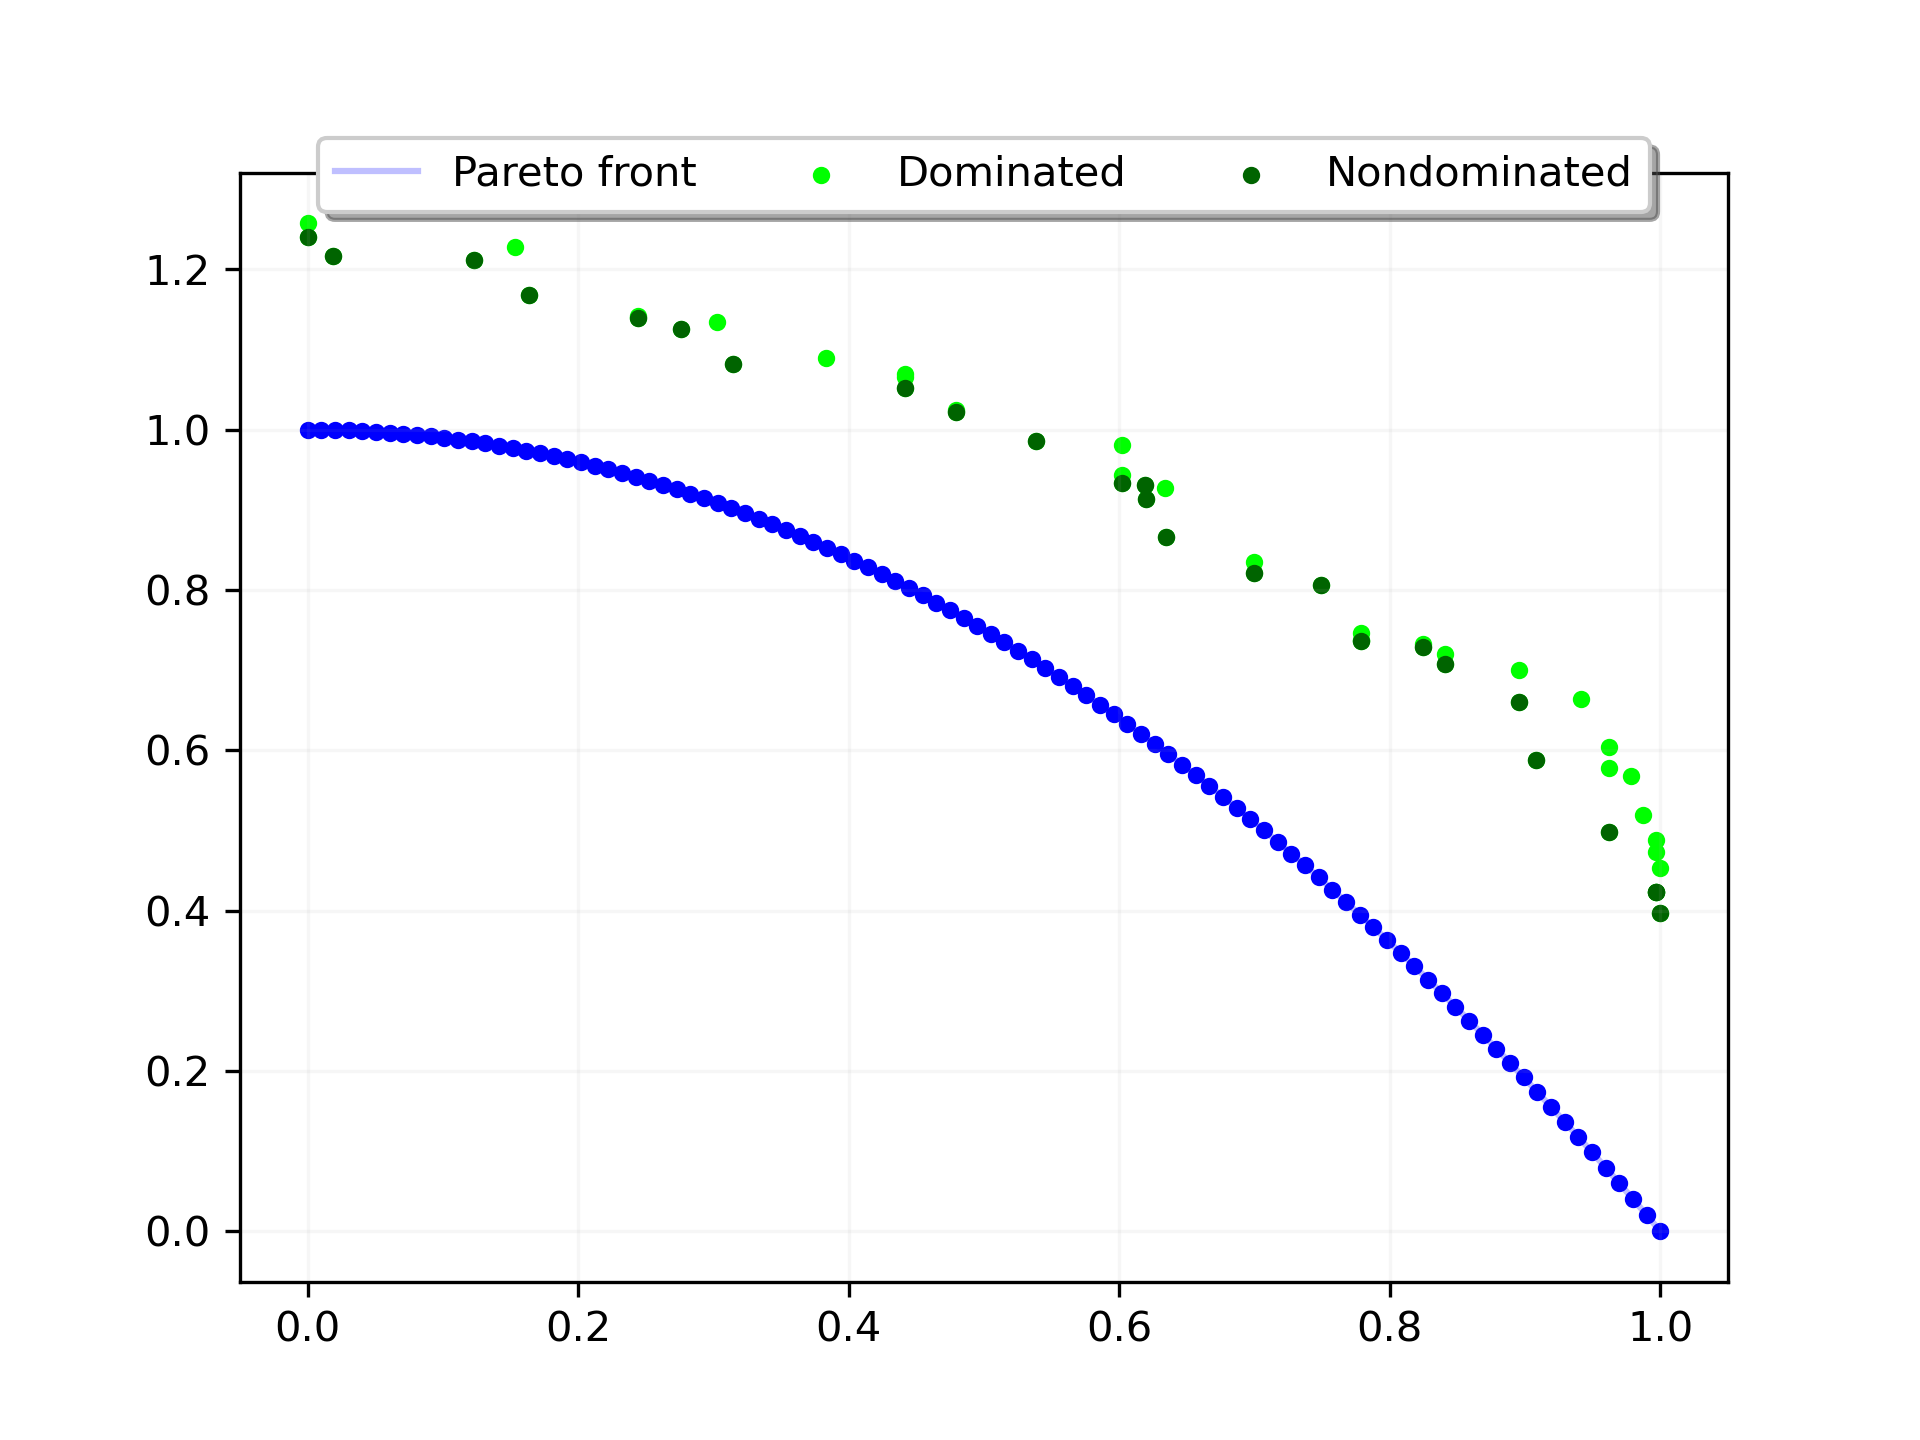
\includegraphics[width=0.9\textwidth]{img2/SPEAII_ZDT2_g10000_p50_r0,25.png}
    \caption{Algorytm SPEA-II, problem ZDT2, \newline generacje - 10 000, populacja - 50, prawdopodobieństwo - 0,25}
\end{figure}

\begin{figure}[H]
    \centering
    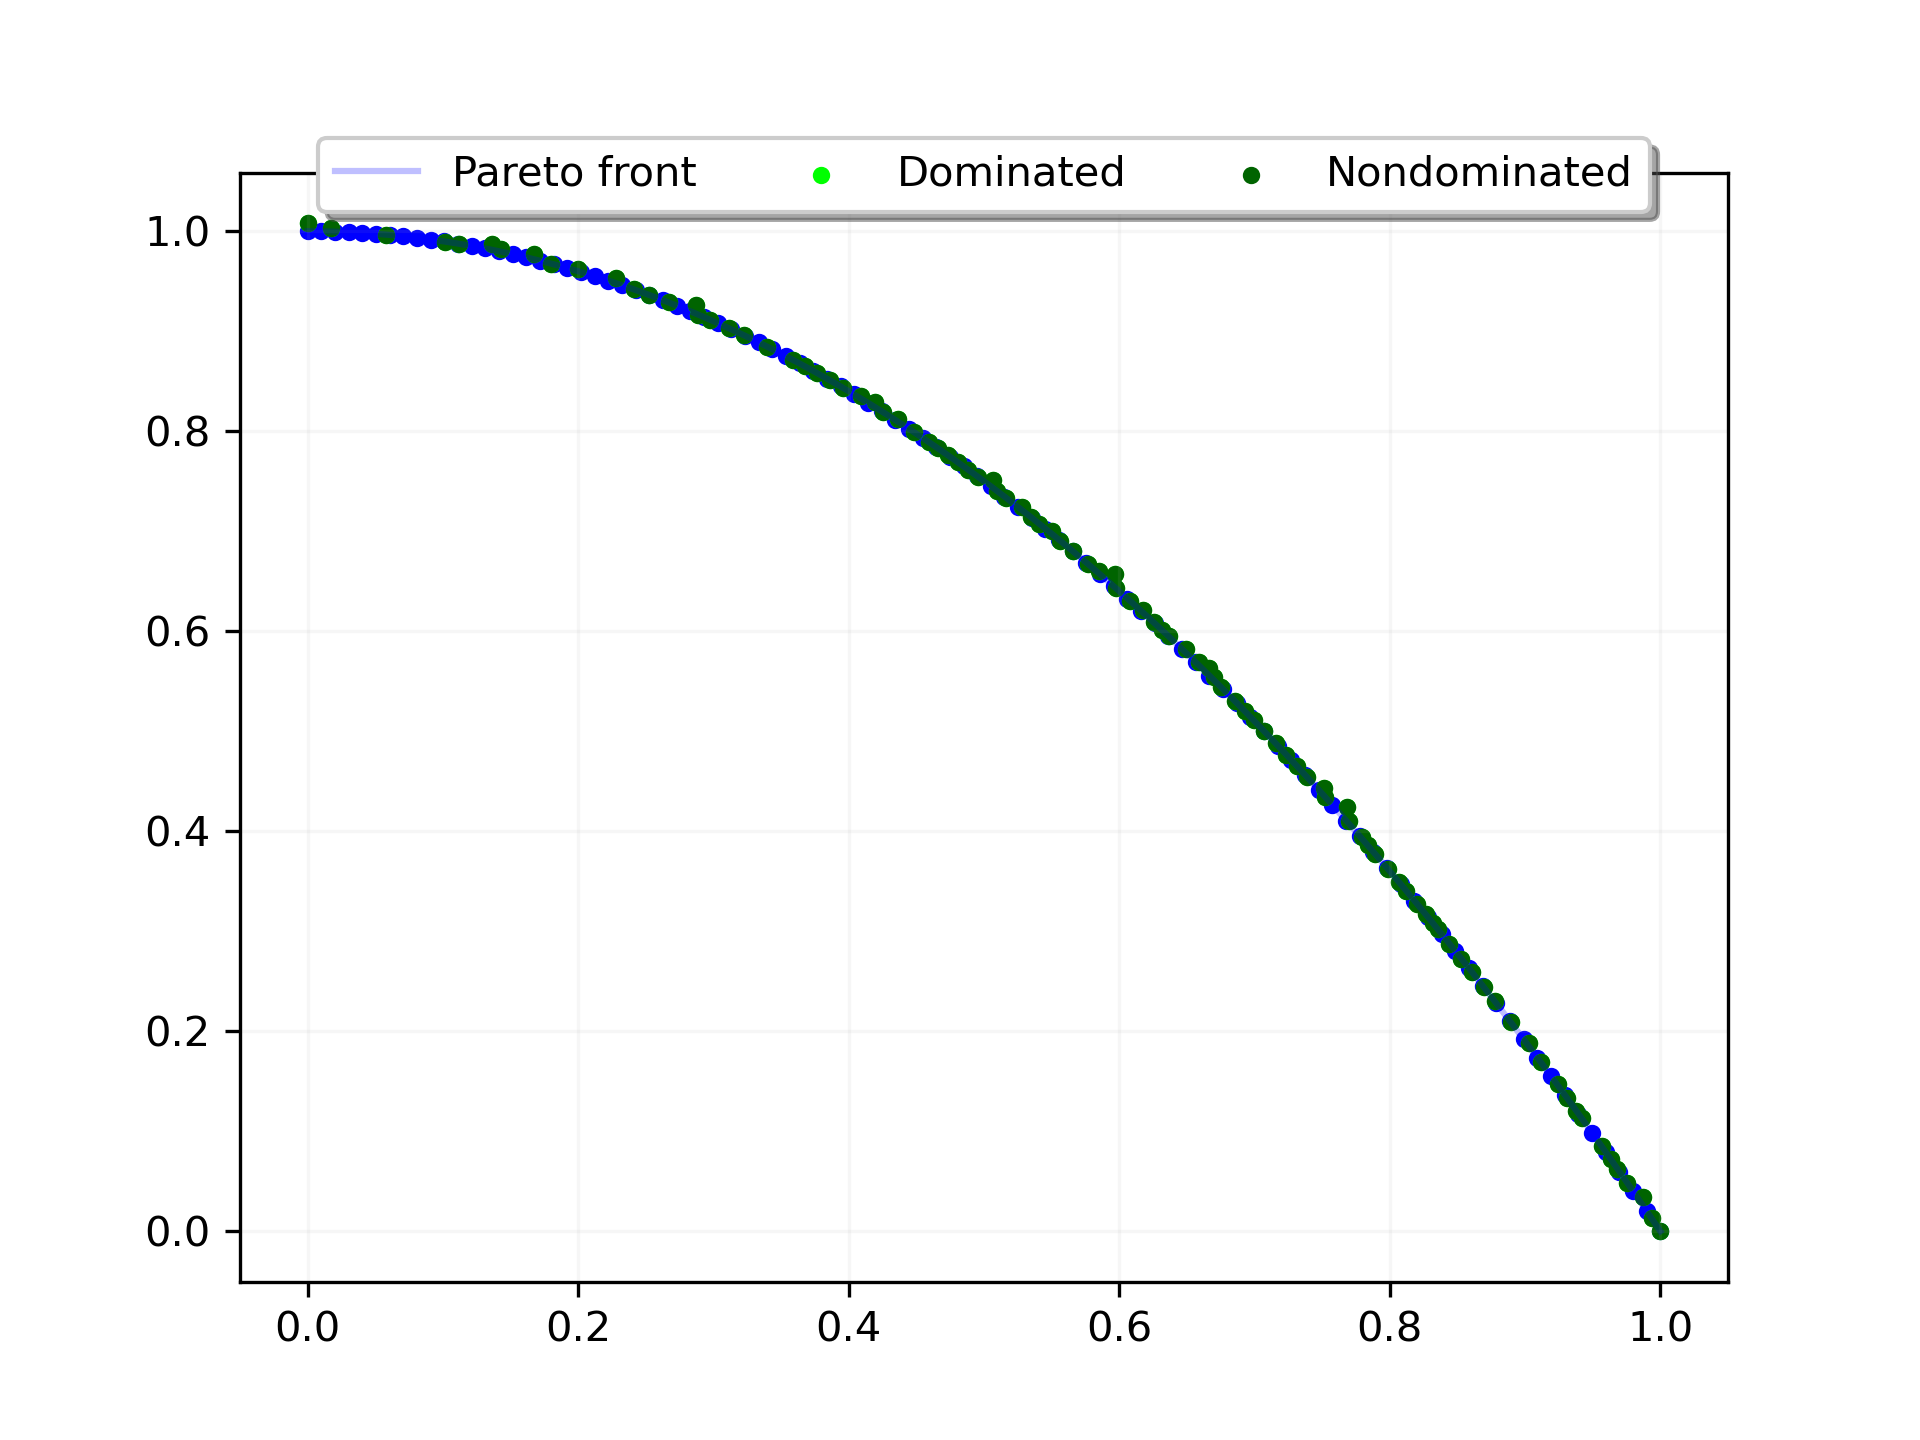
\includegraphics[width=0.9\textwidth]{img2/SPEAII_ZDT2_g100000_p100_r0,25.png}
    \caption{Algorytm SPEA-II, problem ZDT2, \newline generacje - 100 000, populacja - 100, prawdopodobieństwo - 0,25}
\end{figure}

\subsubsection{Problem testowy ZDT3}

\begin{table}[H]
\centering
\caption{Wyniki algorytmu SPEA-II dla problemu ZDT3}
\label{tab:SPEAII_ZDT3}
\begin{tabular}{|ccc|c|c|}
\hline
\textbf{Generacje} & \textbf{Populacja} & \textbf{Prawdo.} & \textbf{GD} & \textbf{HV} \\ \hline
1000 & 50 & 0,25 & 1,891 & 2,458 \\ \hline
\textbf{1000} & \textbf{50} & \textbf{0,5} & \textbf{1,714} & \textbf{2,727} \\ \hline
1000 & 50 & 0,75 & 1,738 & 2,665 \\ \hline
1000 & 100 & 0,25 & 2,362 & 2,169 \\ \hline
1000 & 100 & 0,5 & 2,13 & 2,246 \\ \hline
1000 & 100 & 0,75 & 2,27 & 2,288 \\ \hline
1000 & 200 & 0,25 & 2,476 & 2,017 \\ \hline
1000 & 200 & 0,5 & 2,318 & 2,045 \\ \hline
1000 & 200 & 0,75 & 2,246 & 2,312 \\ \hline
\textbf{10000} & \textbf{50} & \textbf{0,25} & \textbf{0,143} & \textbf{4,676} \\ \hline
10000 & 50 & 0,5 & 0,175 & 4,613 \\ \hline
10000 & 50 & 0,75 & 0,249 & 4,477 \\ \hline
10000 & 100 & 0,25 & 0,359 & 4,313 \\ \hline
10000 & 100 & 0,5 & 0,506 & 4,18 \\ \hline
10000 & 100 & 0,75 & 0,458 & 4,175 \\ \hline
10000 & 200 & 0,25 & 1,073 & 3,411 \\ \hline
10000 & 200 & 0,5 & 0,986 & 3,508 \\ \hline
10000 & 200 & 0,75 & 0,911 & 3,607 \\ \hline
\textbf{100000} & \textbf{50} & \textbf{0,25} & \textbf{0,006} & \textbf{5,037} \\ \hline
100000 & 50 & 0,5 & 0,017 & 4,975 \\ \hline
100000 & 50 & 0,75 & 0,043 & 4,889 \\ \hline
\textbf{100000} & \textbf{100} & \textbf{0,25} & \textbf{0,006} & \textbf{5,037} \\ \hline
100000 & 100 & 0,5 & 0,018 & 4,958 \\ \hline
100000 & 100 & 0,75 & 0,068 & 4,847 \\ \hline
\end{tabular}
\end{table}

\begin{figure}[H]
    \centering
    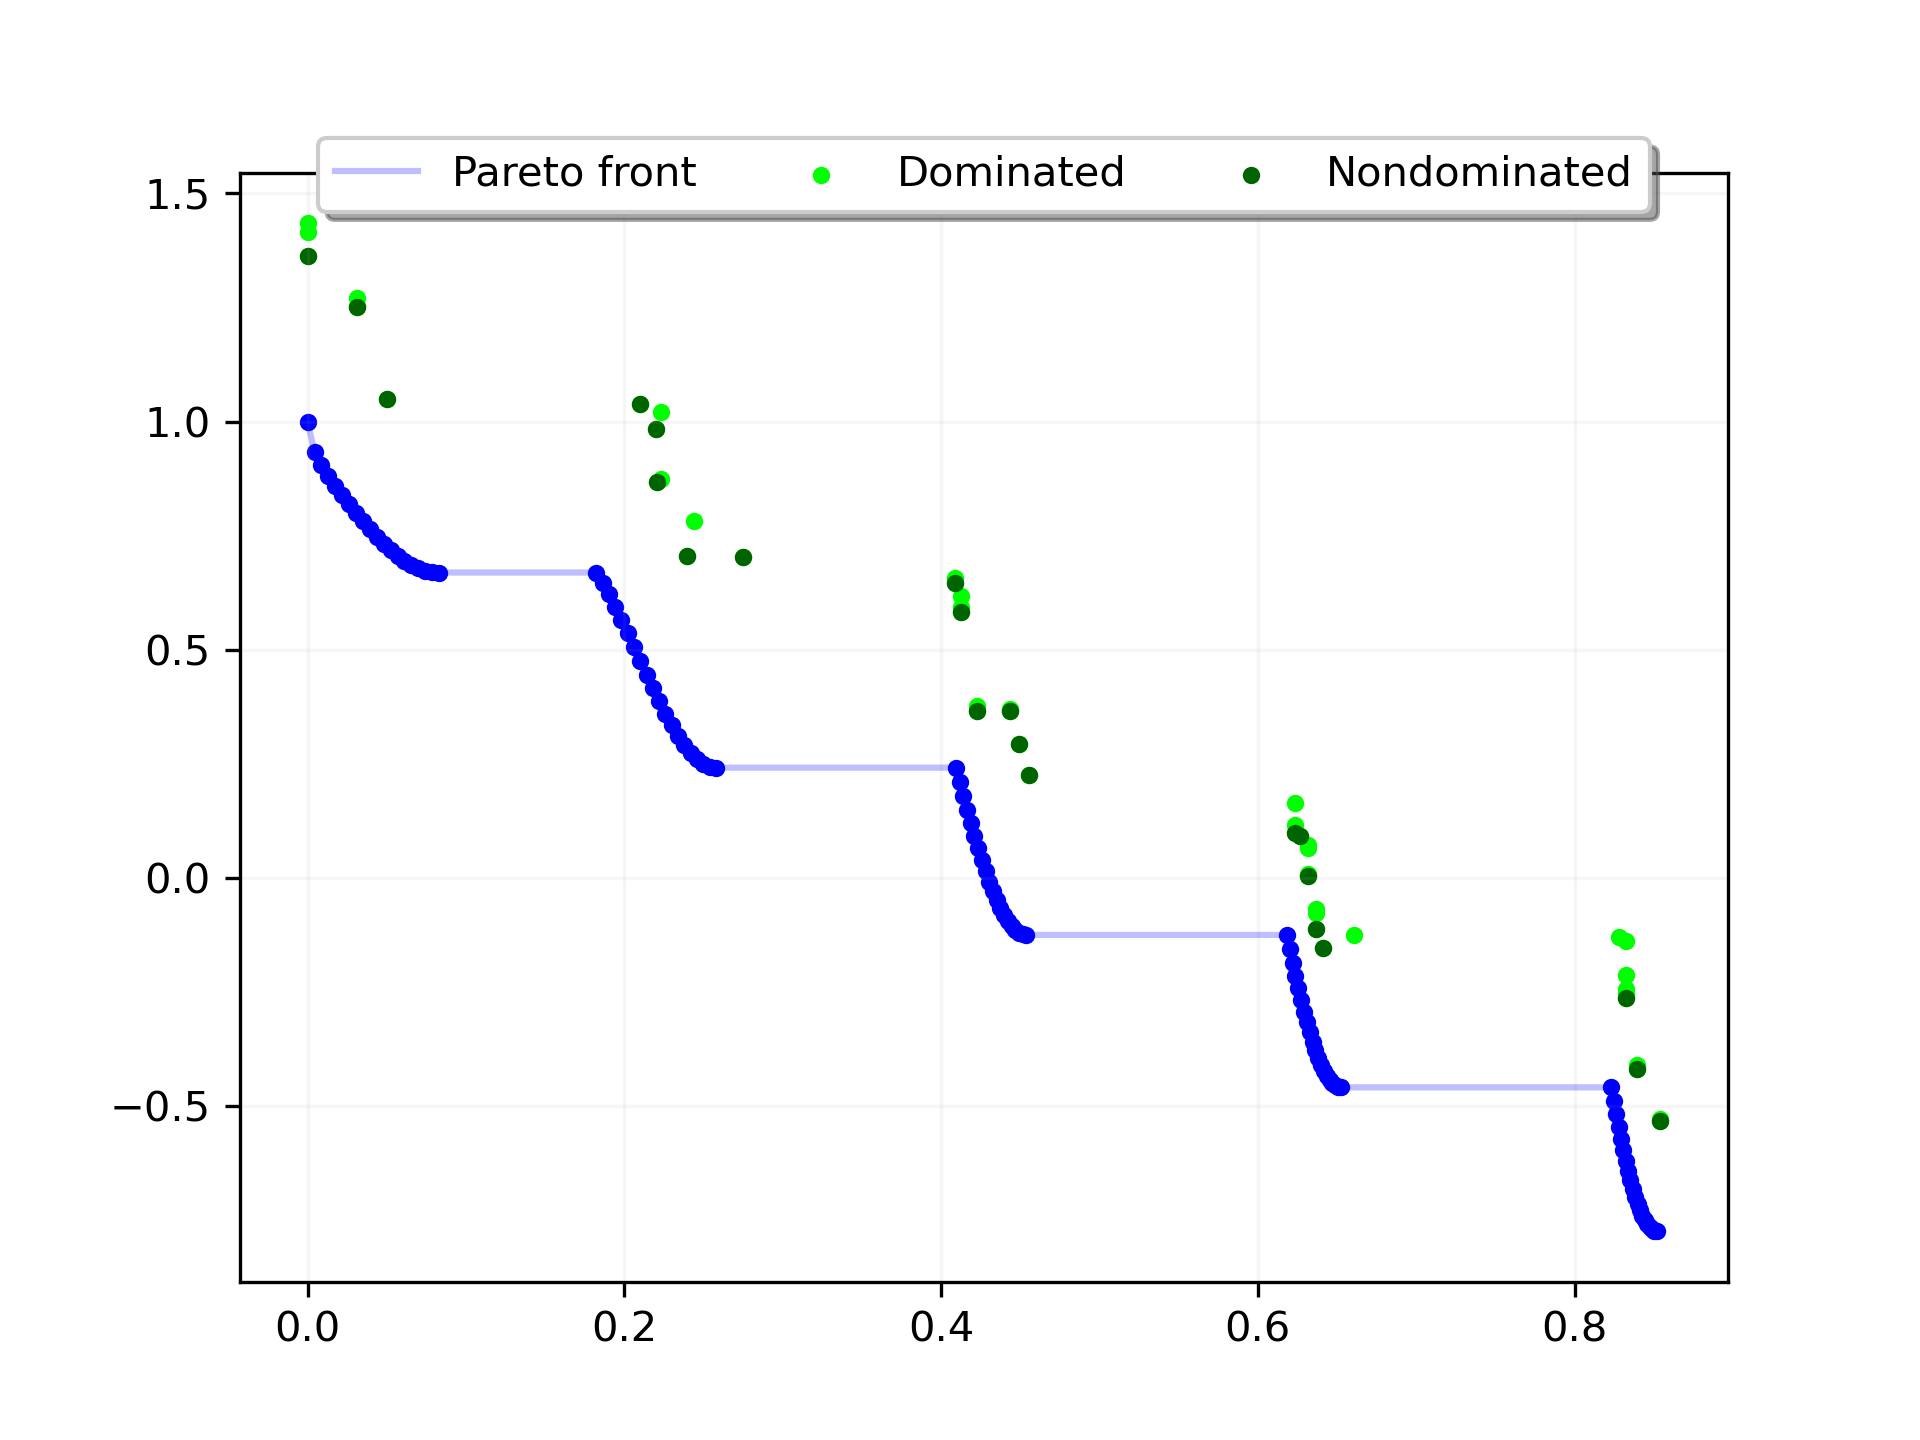
\includegraphics[width=0.9\textwidth]{img2/SPEAII_ZDT3_g10000_p50_r0,25.png}
    \caption{Algorytm SPEA-II, problem ZDT3, \newline generacje - 10 000, populacja - 50, prawdopodobieństwo - 0,25}
\end{figure}

\begin{figure}[H]
    \centering
    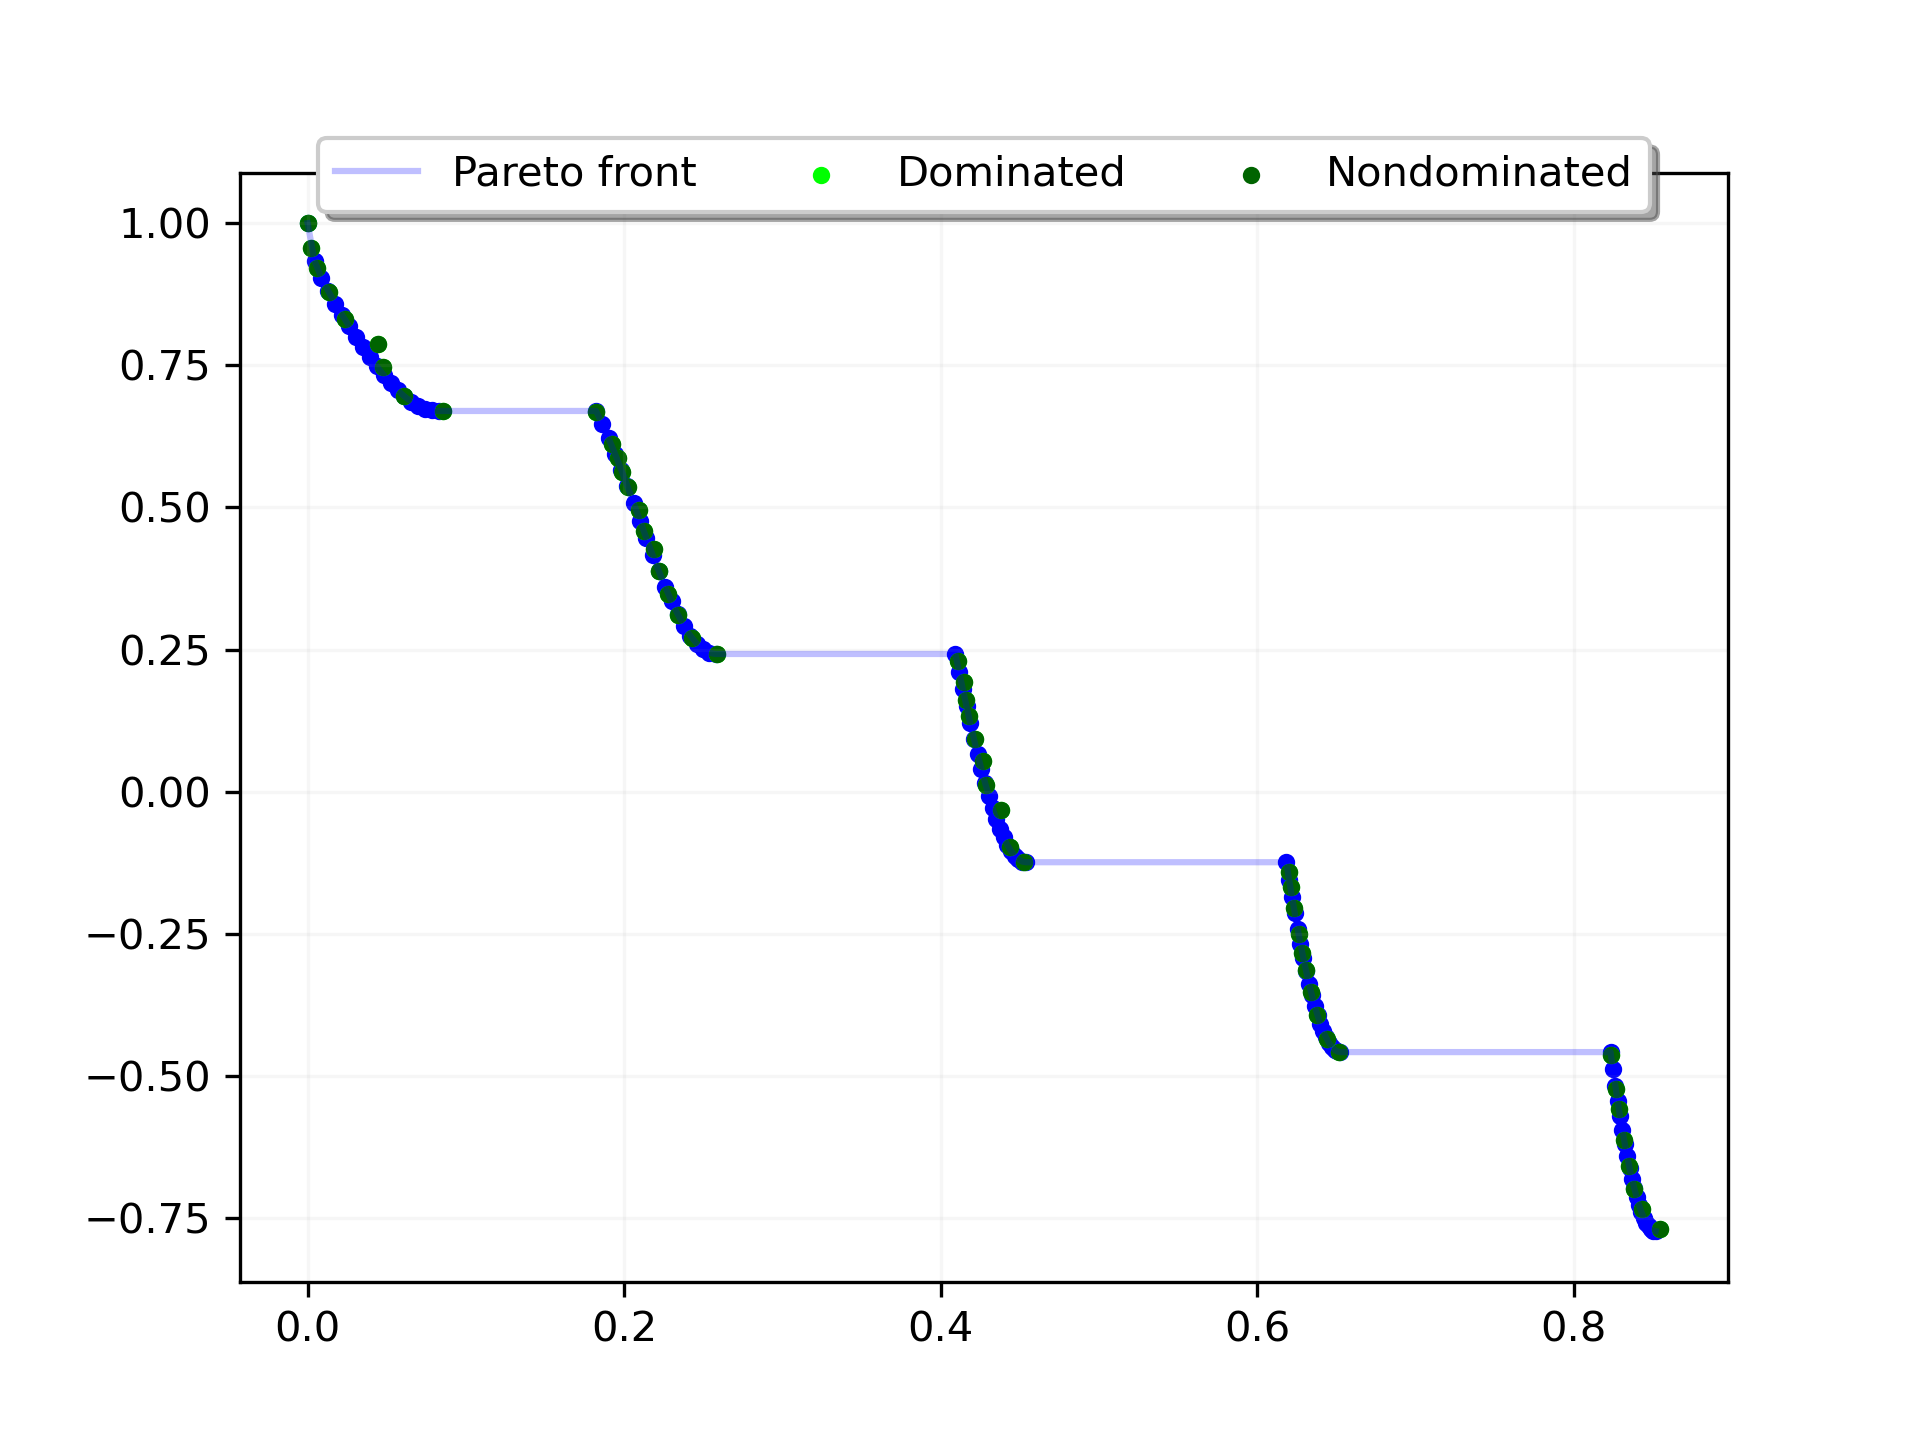
\includegraphics[width=0.9\textwidth]{img2/SPEAII_ZDT3_g100000_p50_r0,25.png}
    \caption{Algorytm SPEA-II, problem ZDT3, \newline generacje - 100 000, populacja - 50, prawdopodobieństwo - 0,25}
\end{figure}

\subsection{Zmiana parametru k}

Parametr k odpowiada za poszukanie k-tego najbliższego punktu na froncie Pareto. Sprawdzono czy zmiana tego parametru (domyślnie jego wartość wynosi 1) wpłynie zauważalnie na rezultaty algorytmu dla ustawień: generacje - 10 000, populacja - 50, prawdopodobieństwo - 0,25.

\begin{table}[H]
\centering
\caption{Wyniki algorytmu SPEA-II (generacje - 10 000, populacja - 50, prawdopodobieństwo - 0,25) dla problemu ZDT1}
\label{tab:SPEAII_e_ZDT1}
\begin{tabular}{|c|c|c|}
\hline
\textbf{k} & \textbf{GD} & \textbf{HV} \\ \hline
\textbf{1} & \textbf{0,164} & \textbf{4,418} \\ \hline
2 & 0,192 & 4,383 \\ \hline
3 & 0,187 & 4,395 \\ \hline
\end{tabular}
\end{table}

\begin{table}[H]
\centering
\caption{Wyniki algorytmu SPEA-II (generacje - 10 000, populacja - 50, prawdopodobieństwo - 0,25) dla problemu ZDT2}
\label{tab:SPEAII_e_ZDT2}
\begin{tabular}{|c|c|c|}
\hline
\textbf{k} & \textbf{GD} & \textbf{HV} \\ \hline
\textbf{1} & \textbf{0,205} & \textbf{4,033} \\ \hline
2 & 0,266 & 3,951 \\ \hline
3 & 0,281 & 3,952 \\ \hline
\end{tabular}
\end{table}

\begin{table}[H]
\centering
\caption{Wyniki algorytmu SPEA-II (generacje - 10 000, populacja - 50, prawdopodobieństwo - 0,25) dla problemu ZDT3}
\label{tab:SPEAII_e_ZDT3}
\begin{tabular}{|l|l|l|}
\hline
\multicolumn{1}{|c|}{\textbf{k}} & \multicolumn{1}{c|}{\textbf{GD}} & \multicolumn{1}{c|}{\textbf{HV}} \\ \hline
1 & 0,143 & 4,676 \\ \hline
2 & 0,128 & 4,705 \\ \hline
\textbf{3} & \textbf{0,089} & \textbf{4,777} \\ \hline
\end{tabular}
\end{table}

\begin{figure}[H]
    \centering
    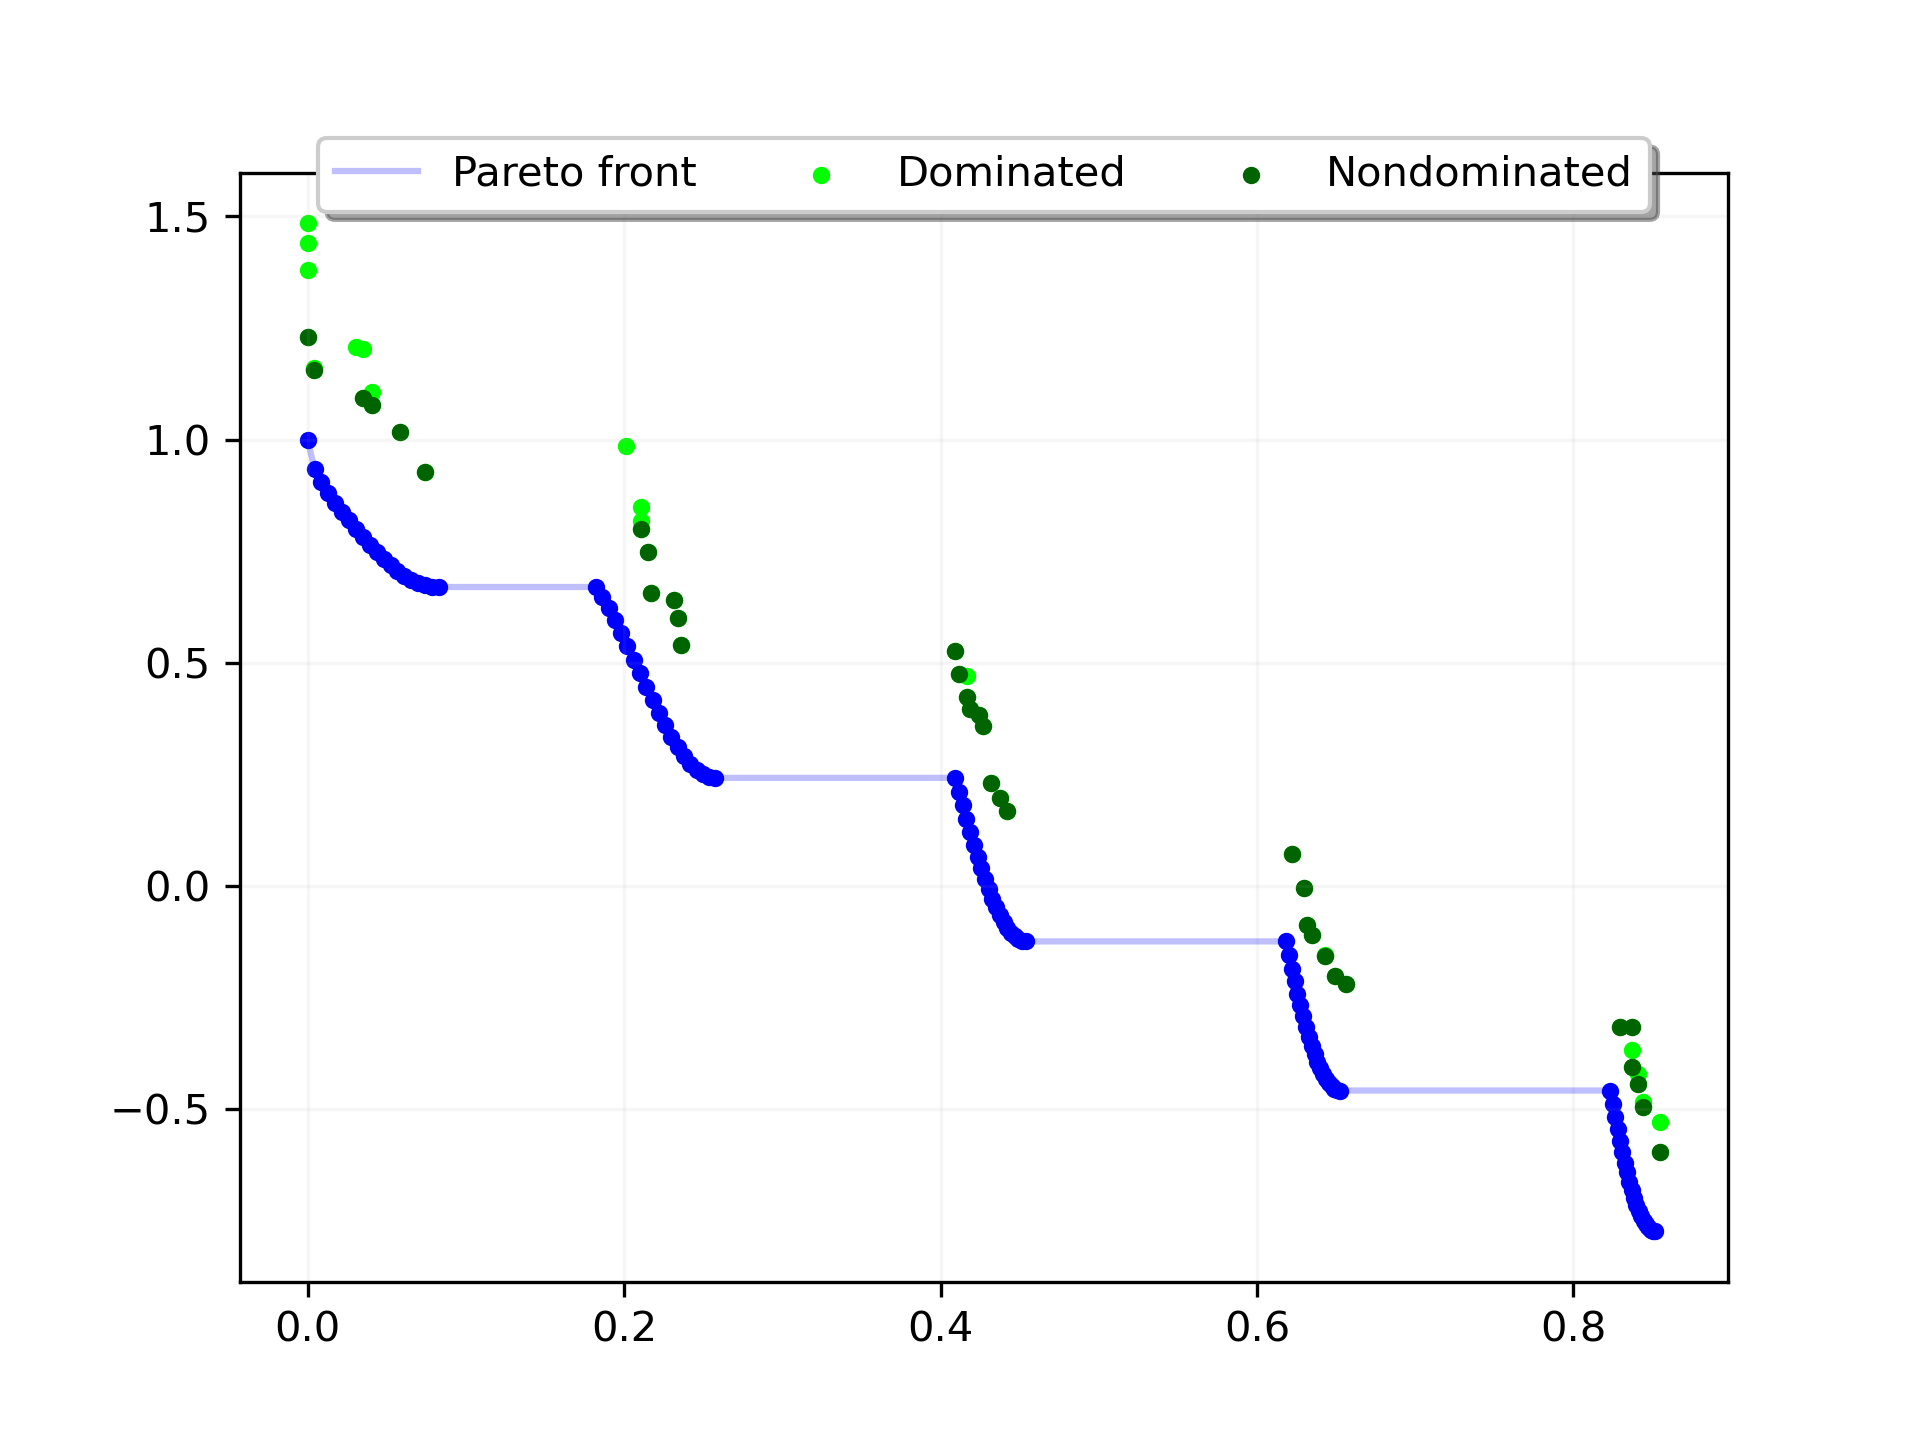
\includegraphics[width=0.9\textwidth]{img2/SPEAII_ZDT3_g10000_p50_r0,25_e3.png}
    \caption{Algorytm SPEA-II, problem ZDT3, \newline generacje - 100 000, populacja - 50, prawdopodobieństwo - 0,25, k - 3}
\end{figure}

\subsection{Algorytm PESA-II}

Ze względu na specyfikację algorytmu PESA-II, na wykresach nie znajdują się zdominowane wyniki.

\subsubsection{Problem testowy ZDT1}

\begin{table}[H]
\centering
\caption{Wyniki algorytmu PESA-II dla problemu ZDT1}
\label{tab:PESAII_ZDT1}
\begin{tabular}{|ccc|c|c|}
\hline
\textbf{Generacje} & \textbf{Populacja} & \textbf{Prawdo.} & \textbf{GD} & \textbf{HV} \\ \hline
1000 & 50 & 0,25 & 0,849 & 3,604 \\ \hline
1000 & 50 & 0,5 & 0,86 & 3,526 \\ \hline
\textbf{1000} & \textbf{50} & \textbf{0,75} & \textbf{0,667} & \textbf{3,74} \\ \hline
1000 & 100 & 0,25 & 1,708 & 2,648 \\ \hline
1000 & 100 & 0,5 & 1,508 & 2,934 \\ \hline
1000 & 100 & 0,75 & 1,186 & 3,281 \\ \hline
1000 & 200 & 0,25 & 2,03 & 2,52 \\ \hline
1000 & 200 & 0,5 & 1,476 & 2,868 \\ \hline
1000 & 200 & 0,75 & 1,742 & 2,603 \\ \hline
\textbf{10000} & \textbf{50} & \textbf{0,25} & \textbf{0,015} & \textbf{4,639} \\ \hline
10000 & 50 & 0,5 & 0,089 & 4,53 \\ \hline
10000 & 50 & 0,75 & 0,143 & 4,45 \\ \hline
10000 & 100 & 0,25 & 0,019 & 4,635 \\ \hline
10000 & 100 & 0,5 & 0,09 & 4,537 \\ \hline
10000 & 100 & 0,75 & 0,182 & 4,397 \\ \hline
10000 & 200 & 0,25 & 0,041 & 4,605 \\ \hline
10000 & 200 & 0,5 & 0,105 & 4,503 \\ \hline
10000 & 200 & 0,75 & 0,173 & 4,403 \\ \hline
\textbf{100000} & \textbf{50} & \textbf{0,25} & \textbf{0,003} & \textbf{4,651} \\ \hline
100000 & 50 & 0,5 & 0,021 & 4,636 \\ \hline
100000 & 50 & 0,75 & 0,063 & 4,564 \\ \hline
\textbf{100000} & \textbf{100} & \textbf{0,25} & \textbf{0,004} & \textbf{4,653} \\ \hline
100000 & 100 & 0,5 & 0,021 & 4,635 \\ \hline
100000 & 100 & 0,75 & 0,078 & 4,549 \\ \hline
100000 & 200 & 0,25 & 0,004 & 4,651 \\ \hline
100000 & 200 & 0,5 & 0,02 & 4,635 \\ \hline
100000 & 200 & 0,75 & 0,065 & 4,566 \\ \hline
\end{tabular}
\end{table}

\begin{figure}[H]
    \centering
    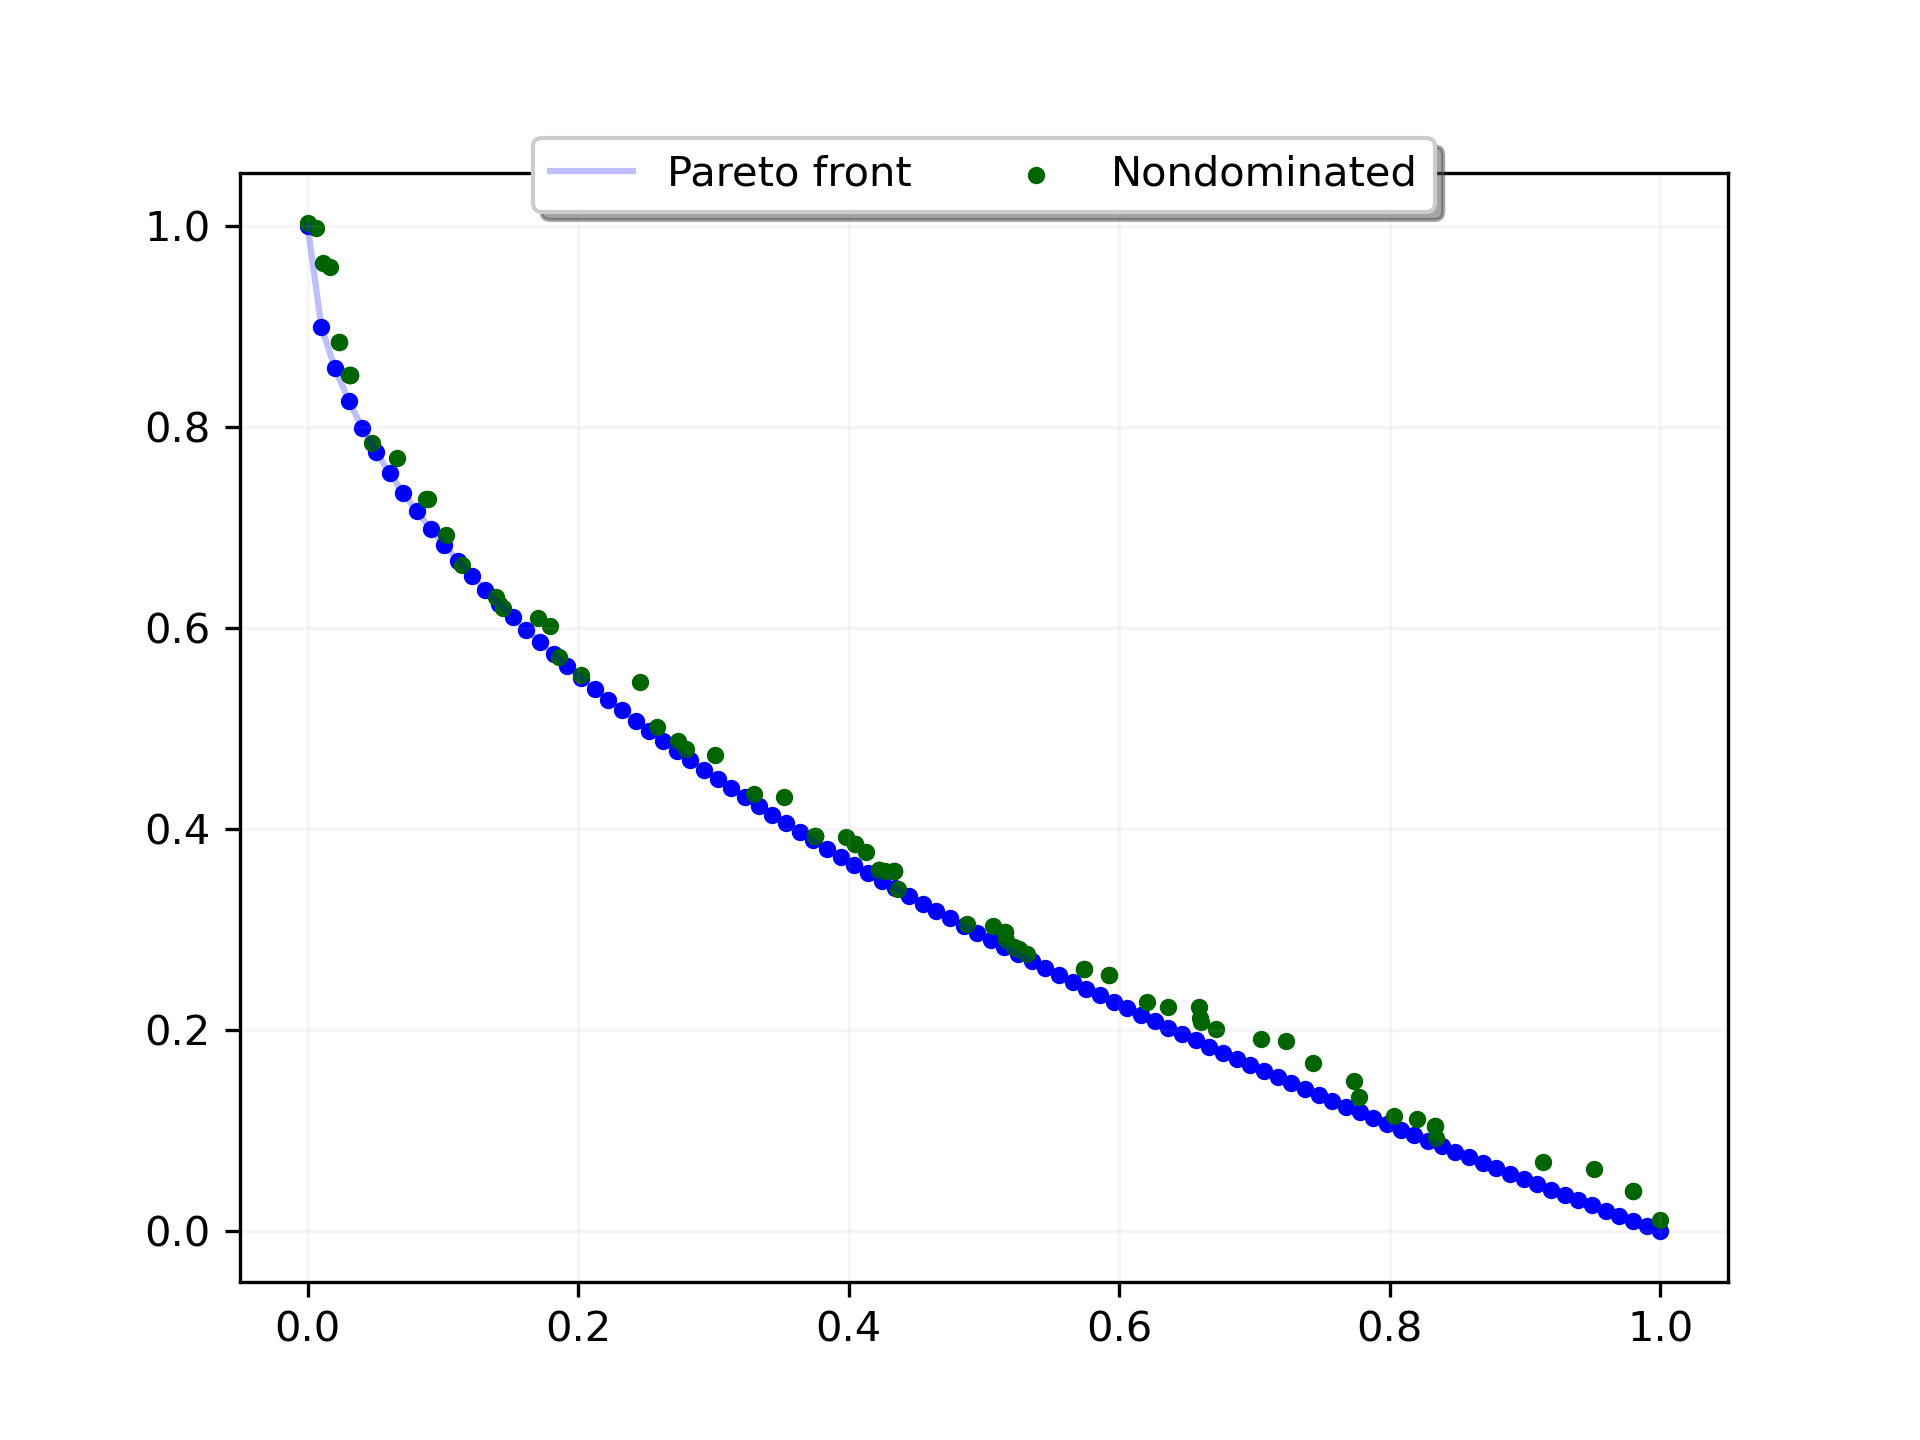
\includegraphics[width=0.9\textwidth]{img2/PESAII_ZDT1_g10000_p50_r0,25.png}
    \caption{Algorytm PESA-II, problem ZDT1, \newline generacje - 10 000, populacja - 50, prawdopodobieństwo - 0,25}
\end{figure}

\begin{figure}[H]
    \centering
    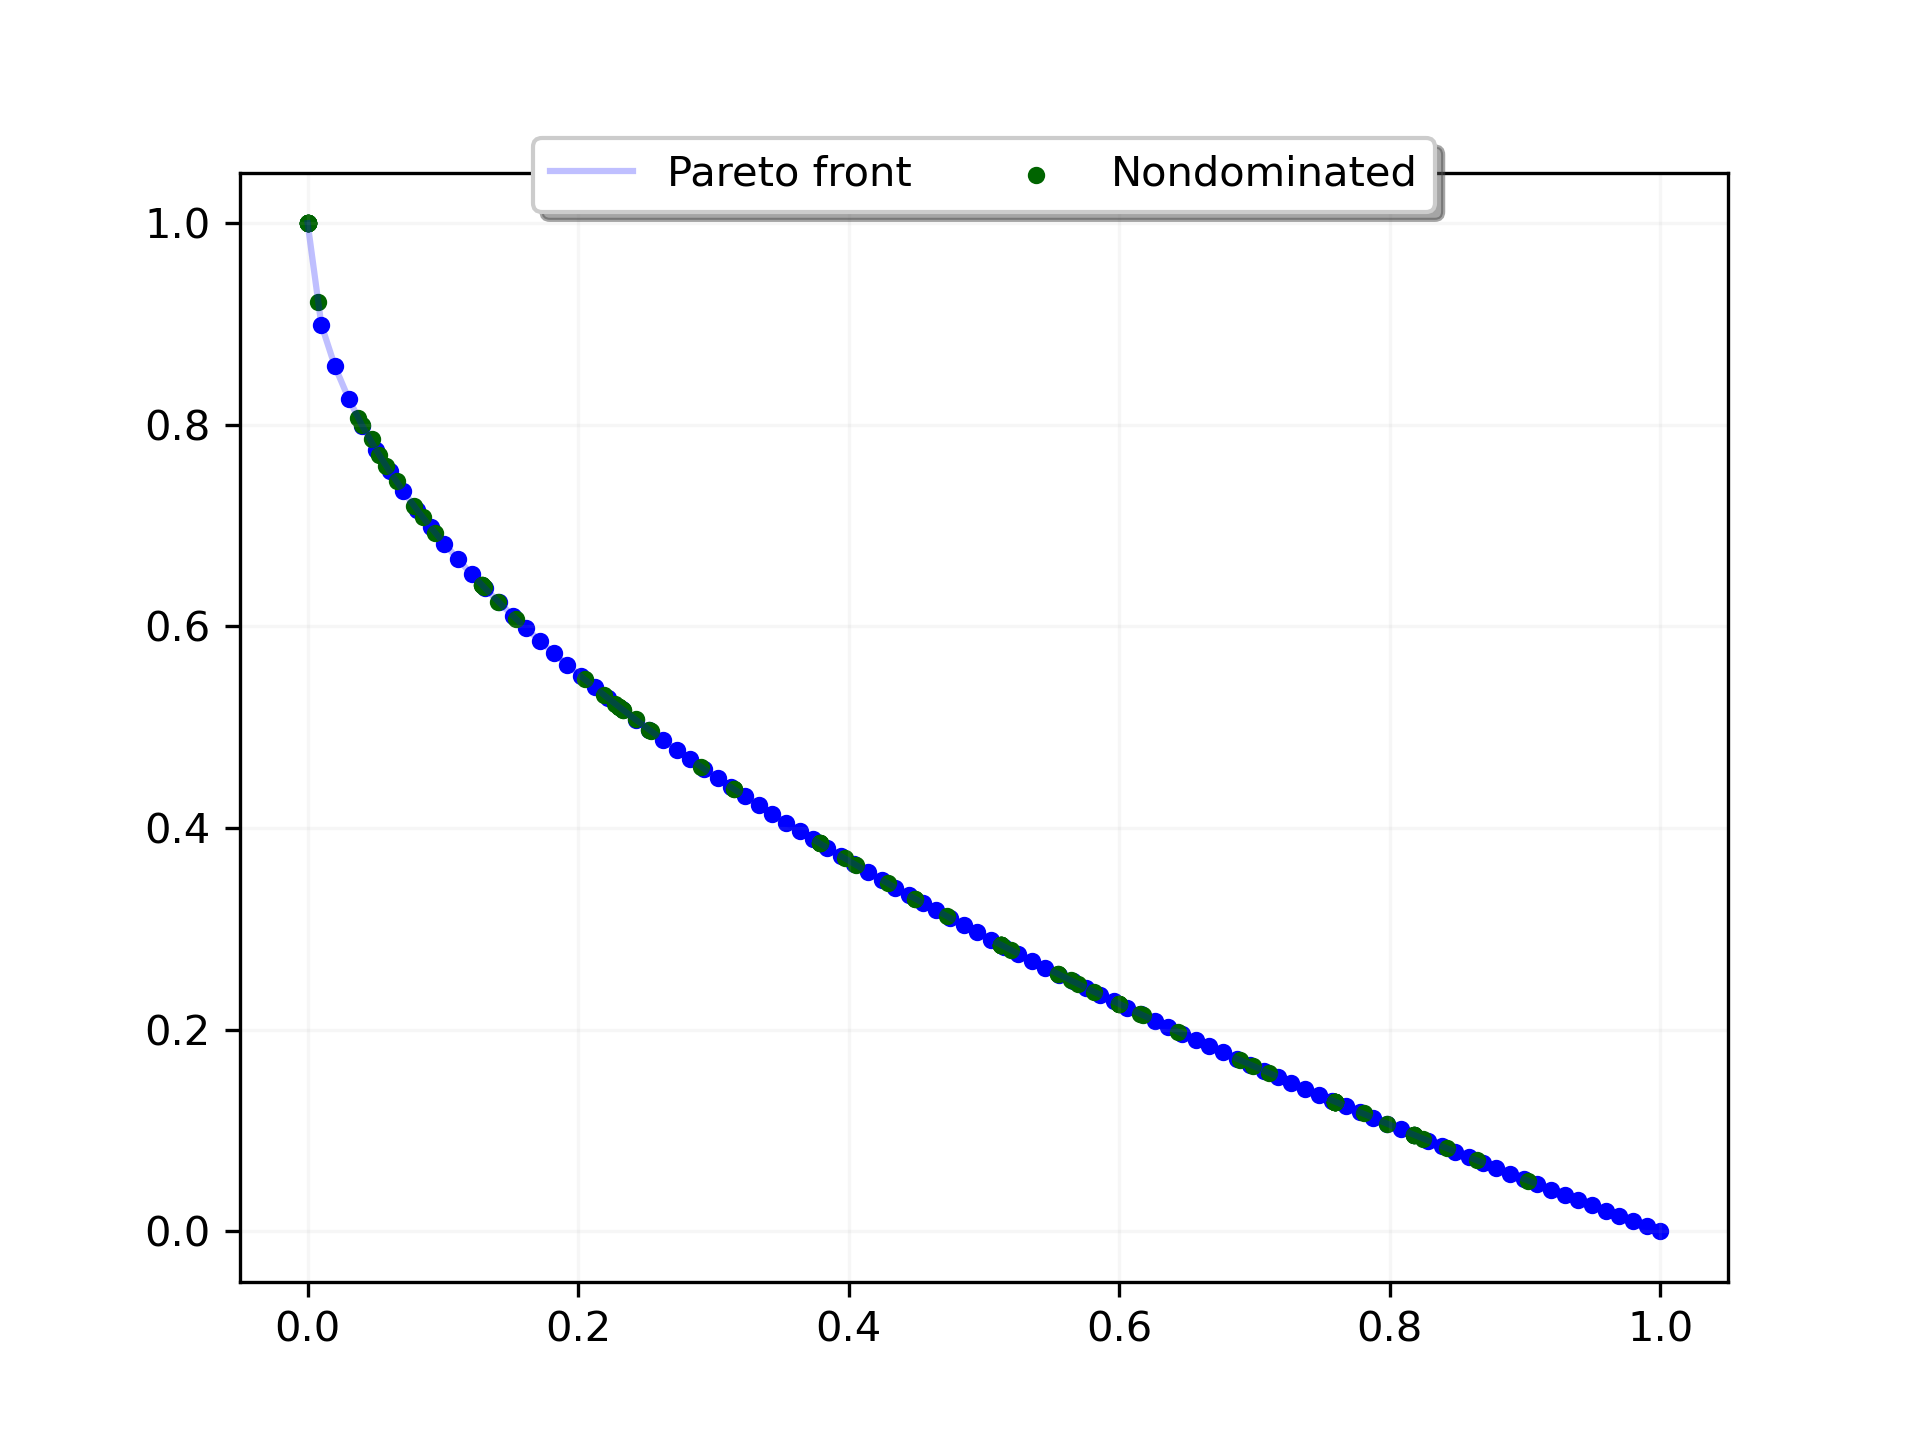
\includegraphics[width=0.9\textwidth]{img2/PESAII_ZDT1_g100000_p50_r0,25.png}
    \caption{Algorytm PESA-II, problem ZDT1, \newline generacje - 100 000, populacja - 50, prawdopodobieństwo - 0,25}
\end{figure}

\subsubsection{Problem testowy ZDT2}

\begin{table}[H]
\centering
\caption{Wyniki algorytmu PESA-II dla problemu ZDT2}
\label{tab:PESAII_ZDT2}
\begin{tabular}{|ccc|c|c|}
\hline
\textbf{Generacje} & \textbf{Populacja} & \textbf{Prawdo.} & \textbf{GD} & \textbf{HV} \\ \hline
1000 & 50 & 0,25 & 1,127 & 2,996 \\ \hline
\textbf{1000} & \textbf{50} & \textbf{0,5} & \textbf{0,496} & \textbf{3,504} \\ \hline
1000 & 50 & 0,75 & 0,884 & 3,177 \\ \hline
1000 & 100 & 0,25 & 1,616 & 2,454 \\ \hline
1000 & 100 & 0,5 & 1,303 & 2,715 \\ \hline
1000 & 100 & 0,75 & 1,066 & 2,934 \\ \hline
1000 & 200 & 0,25 & 2,701 & 1,408 \\ \hline
1000 & 200 & 0,5 & 1,912 & 2,206 \\ \hline
1000 & 200 & 0,75 & 1,757 & 2,304 \\ \hline
\textbf{10000} & \textbf{50} & \textbf{0,25} & \textbf{0,011} & \textbf{4,31} \\ \hline
10000 & 50 & 0,5 & 0,11 & 4,174 \\ \hline
10000 & 50 & 0,75 & 0,22 & 4,008 \\ \hline
10000 & 100 & 0,25 & 0,012 & 4,305 \\ \hline
10000 & 100 & 0,5 & 0,088 & 4,189 \\ \hline
10000 & 100 & 0,75 & 0,198 & 4,032 \\ \hline
10000 & 200 & 0,25 & 0,038 & 4,27 \\ \hline
10000 & 200 & 0,5 & 0,105 & 4,165 \\ \hline
10000 & 200 & 0,75 & 0,229 & 3,988 \\ \hline
\textbf{100000} & \textbf{50} & \textbf{0,25} & \textbf{0,004} & \textbf{4,32} \\ \hline
100000 & 50 & 0,5 & 0,022 & 4,295 \\ \hline
100000 & 50 & 0,75 & 0,092 & 4,185 \\ \hline
\textbf{100000} & \textbf{100} & \textbf{0,25} & \textbf{0,004} & \textbf{4,32} \\ \hline
100000 & 100 & 0,5 & 0,025 & 4,289 \\ \hline
100000 & 100 & 0,75 & 0,1 & 4,183 \\ \hline
100000 & 200 & 0,25 & 0,005 & 4,321 \\ \hline
100000 & 200 & 0,5 & 0,018 & 4,299 \\ \hline
100000 & 200 & 0,75 & 0,117 & 4,159 \\ \hline
\end{tabular}
\end{table}

\begin{figure}[H]
    \centering
    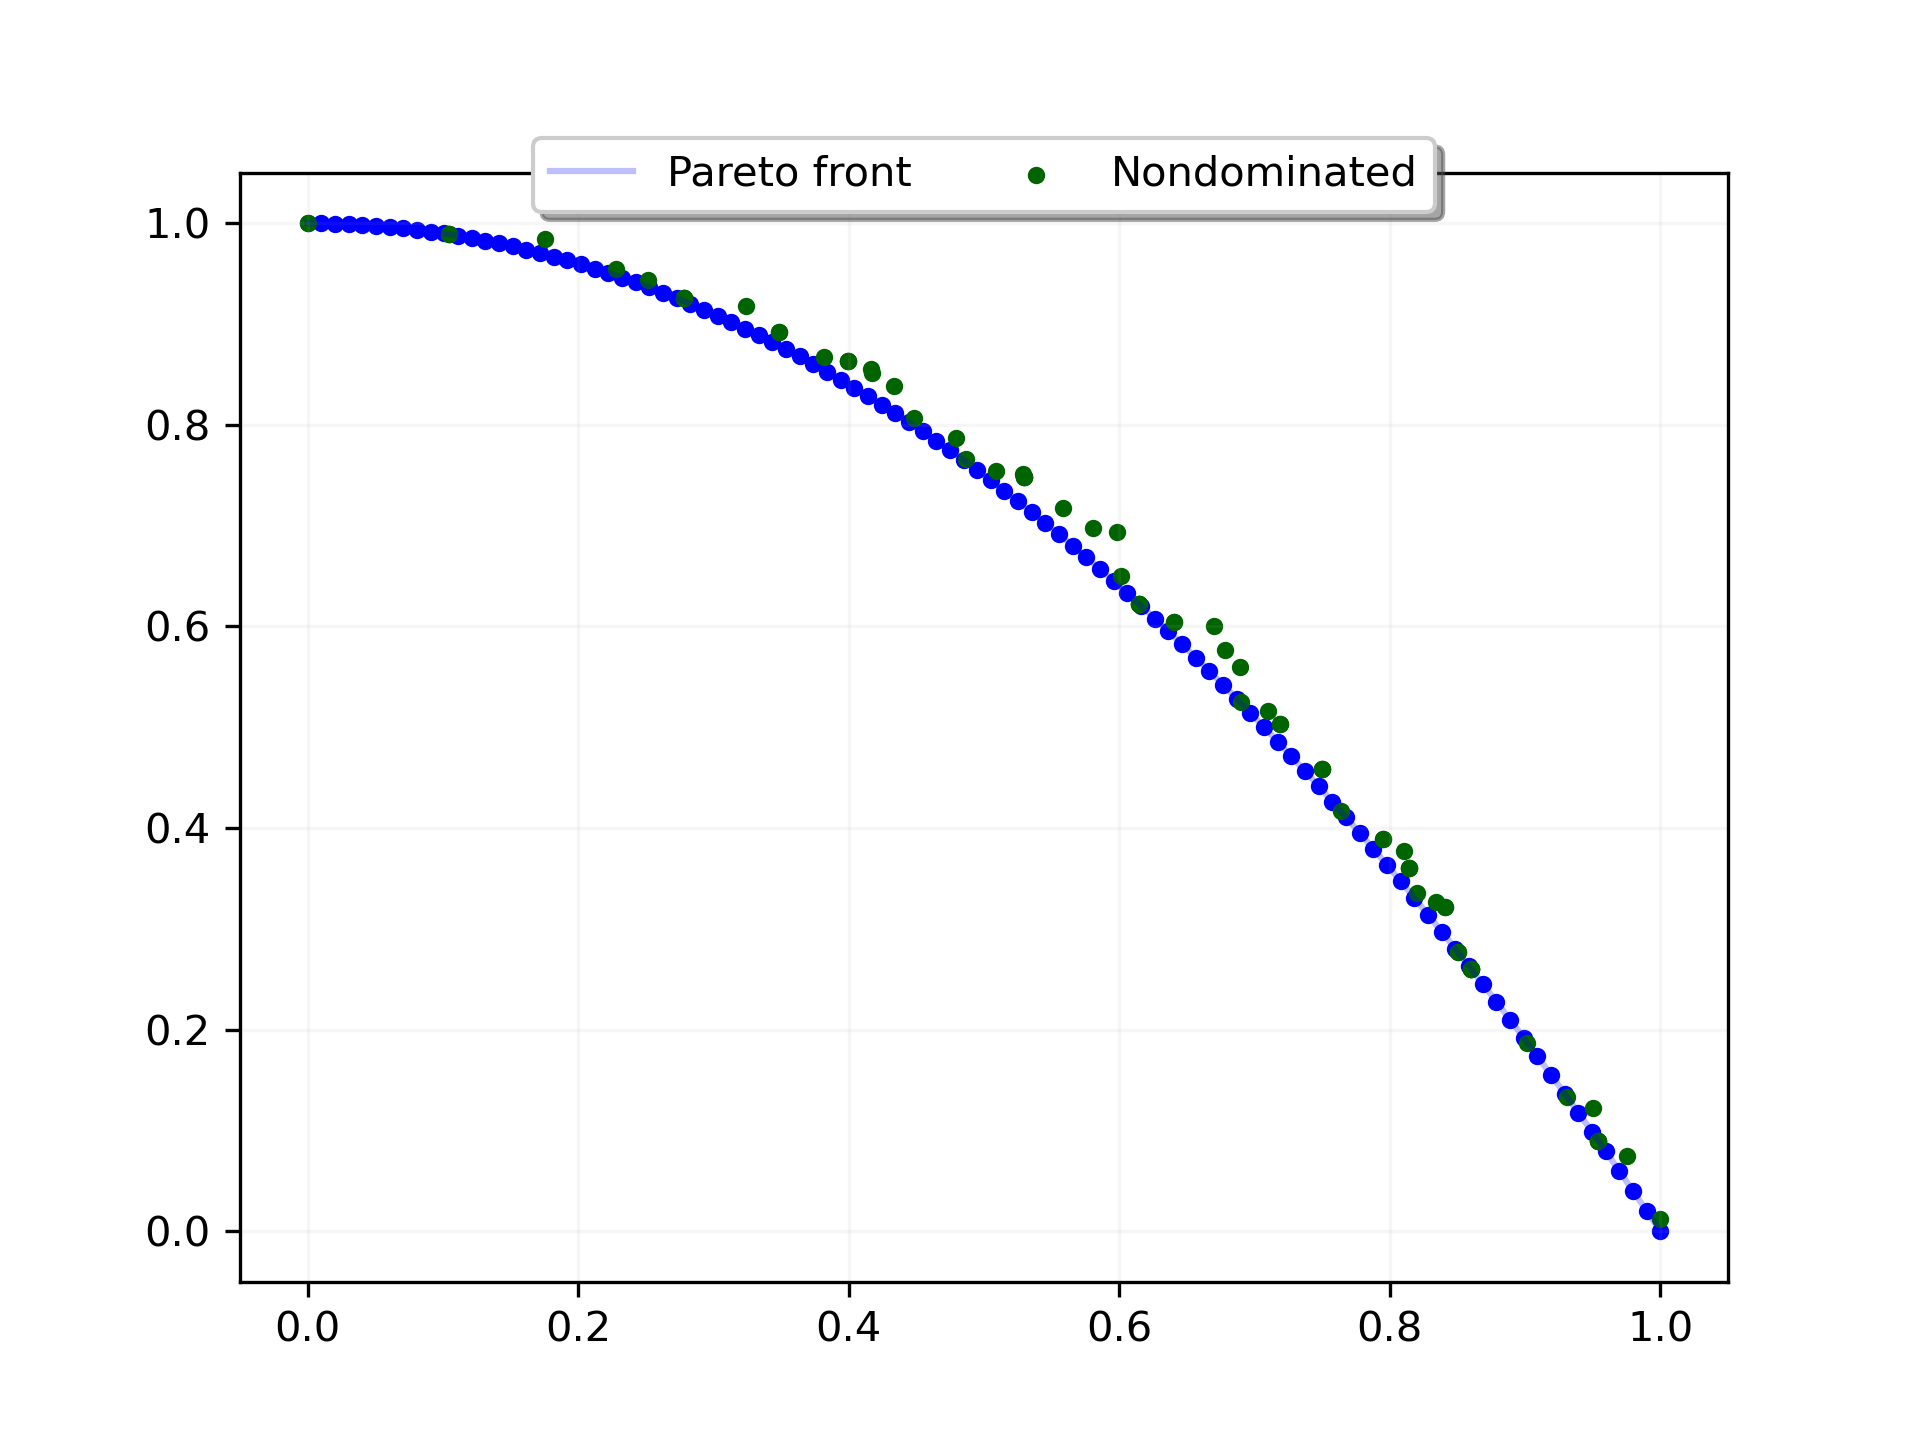
\includegraphics[width=0.9\textwidth]{img2/PESAII_ZDT2_g10000_p50_r0,25.png}
    \caption{Algorytm PESA-II, problem ZDT2, \newline generacje - 10 000, populacja - 50, prawdopodobieństwo - 0,25}
\end{figure}

\begin{figure}[H]
    \centering
    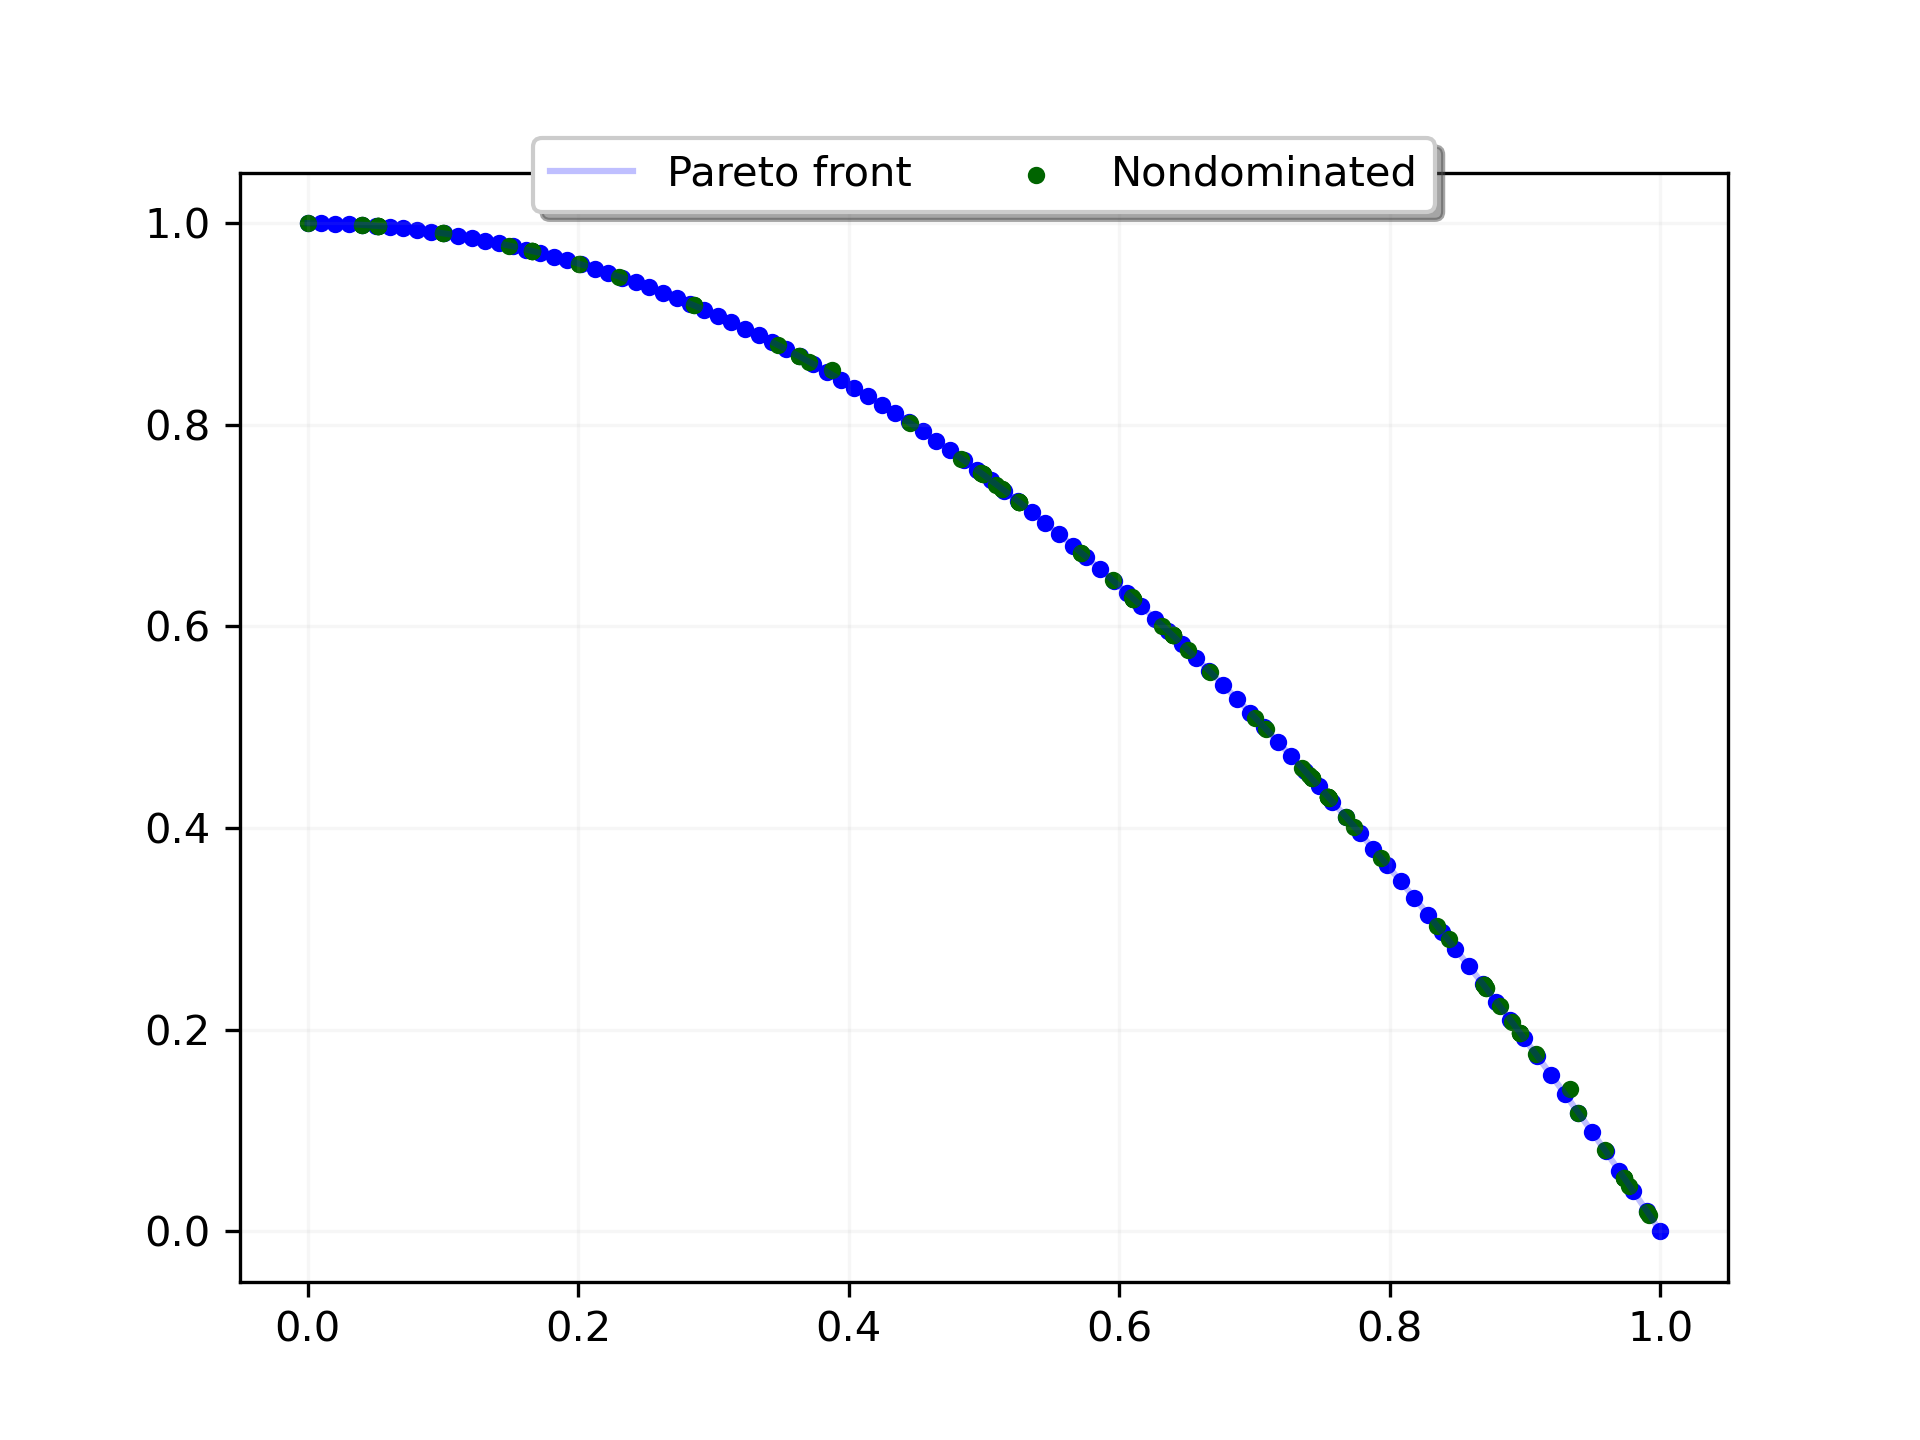
\includegraphics[width=0.9\textwidth]{img2/PESAII_ZDT2_g100000_p50_r0,25.png}
    \caption{Algorytm PESA-II, problem ZDT2, \newline generacje - 100 000, populacja - 50, prawdopodobieństwo - 0,25}
\end{figure}

\subsubsection{Problem testowy ZDT3}

\begin{table}[H]
\centering
\caption{Wyniki algorytmu PESA-II dla problemu ZDT3}
\label{tab:PESAII_ZDT3}
\begin{tabular}{|ccc|c|c|}
\hline
\textbf{Generacje} & \textbf{Populacja} & \textbf{Prawdo.} & \textbf{GD} & \textbf{HV} \\ \hline
1000 & 50 & 0,25 & 1,264 & 3,313 \\ \hline
1000 & 50 & 0,5 & 0,752 & 3,766 \\ \hline
\textbf{1000} & \textbf{50} & \textbf{0,75} & \textbf{0,67} & \textbf{3,799} \\ \hline
1000 & 100 & 0,25 & 1,083 & 3,334 \\ \hline
1000 & 100 & 0,5 & 0,991 & 3,449 \\ \hline
1000 & 100 & 0,75 & 1,194 & 3,348 \\ \hline
1000 & 200 & 0,25 & 1,534 & 3,158 \\ \hline
1000 & 200 & 0,5 & 1,317 & 3,06 \\ \hline
1000 & 200 & 0,75 & 1,448 & 3,023 \\ \hline
\textbf{10000} & \textbf{50} & \textbf{0,25} & \textbf{0,013} & \textbf{4,991} \\ \hline
10000 & 50 & 0,5 & 0,039 & 4,915 \\ \hline
10000 & 50 & 0,75 & 0,126 & 4,703 \\ \hline
10000 & 100 & 0,25 & 0,02 & 4,977 \\ \hline
10000 & 100 & 0,5 & 0,082 & 4,815 \\ \hline
10000 & 100 & 0,75 & 0,12 & 4,746 \\ \hline
10000 & 200 & 0,25 & 0,023 & 4,922 \\ \hline
10000 & 200 & 0,5 & 0,068 & 4,877 \\ \hline
10000 & 200 & 0,75 & 0,104 & 4,749 \\ \hline
\textbf{100000} & \textbf{50} & \textbf{0,25} & \textbf{0,006} & \textbf{5,034} \\ \hline
100000 & 50 & 0,5 & 0,012 & 5,006 \\ \hline
100000 & 50 & 0,75 & 0,037 & 4,902 \\ \hline
100000 & 100 & 0,25 & 0,005 & 5,031 \\ \hline
100000 & 100 & 0,5 & 0,01 & 5,007 \\ \hline
100000 & 100 & 0,75 & 0,033 & 4,929 \\ \hline
\textbf{100000} & \textbf{200} & \textbf{0,25} & \textbf{0,005} & \textbf{5,032} \\ \hline
100000 & 200 & 0,5 & 0,011 & 4,996 \\ \hline
100000 & 200 & 0,75 & 0,044 & 4,92 \\ \hline
\end{tabular}
\end{table}

\begin{figure}[H]
    \centering
    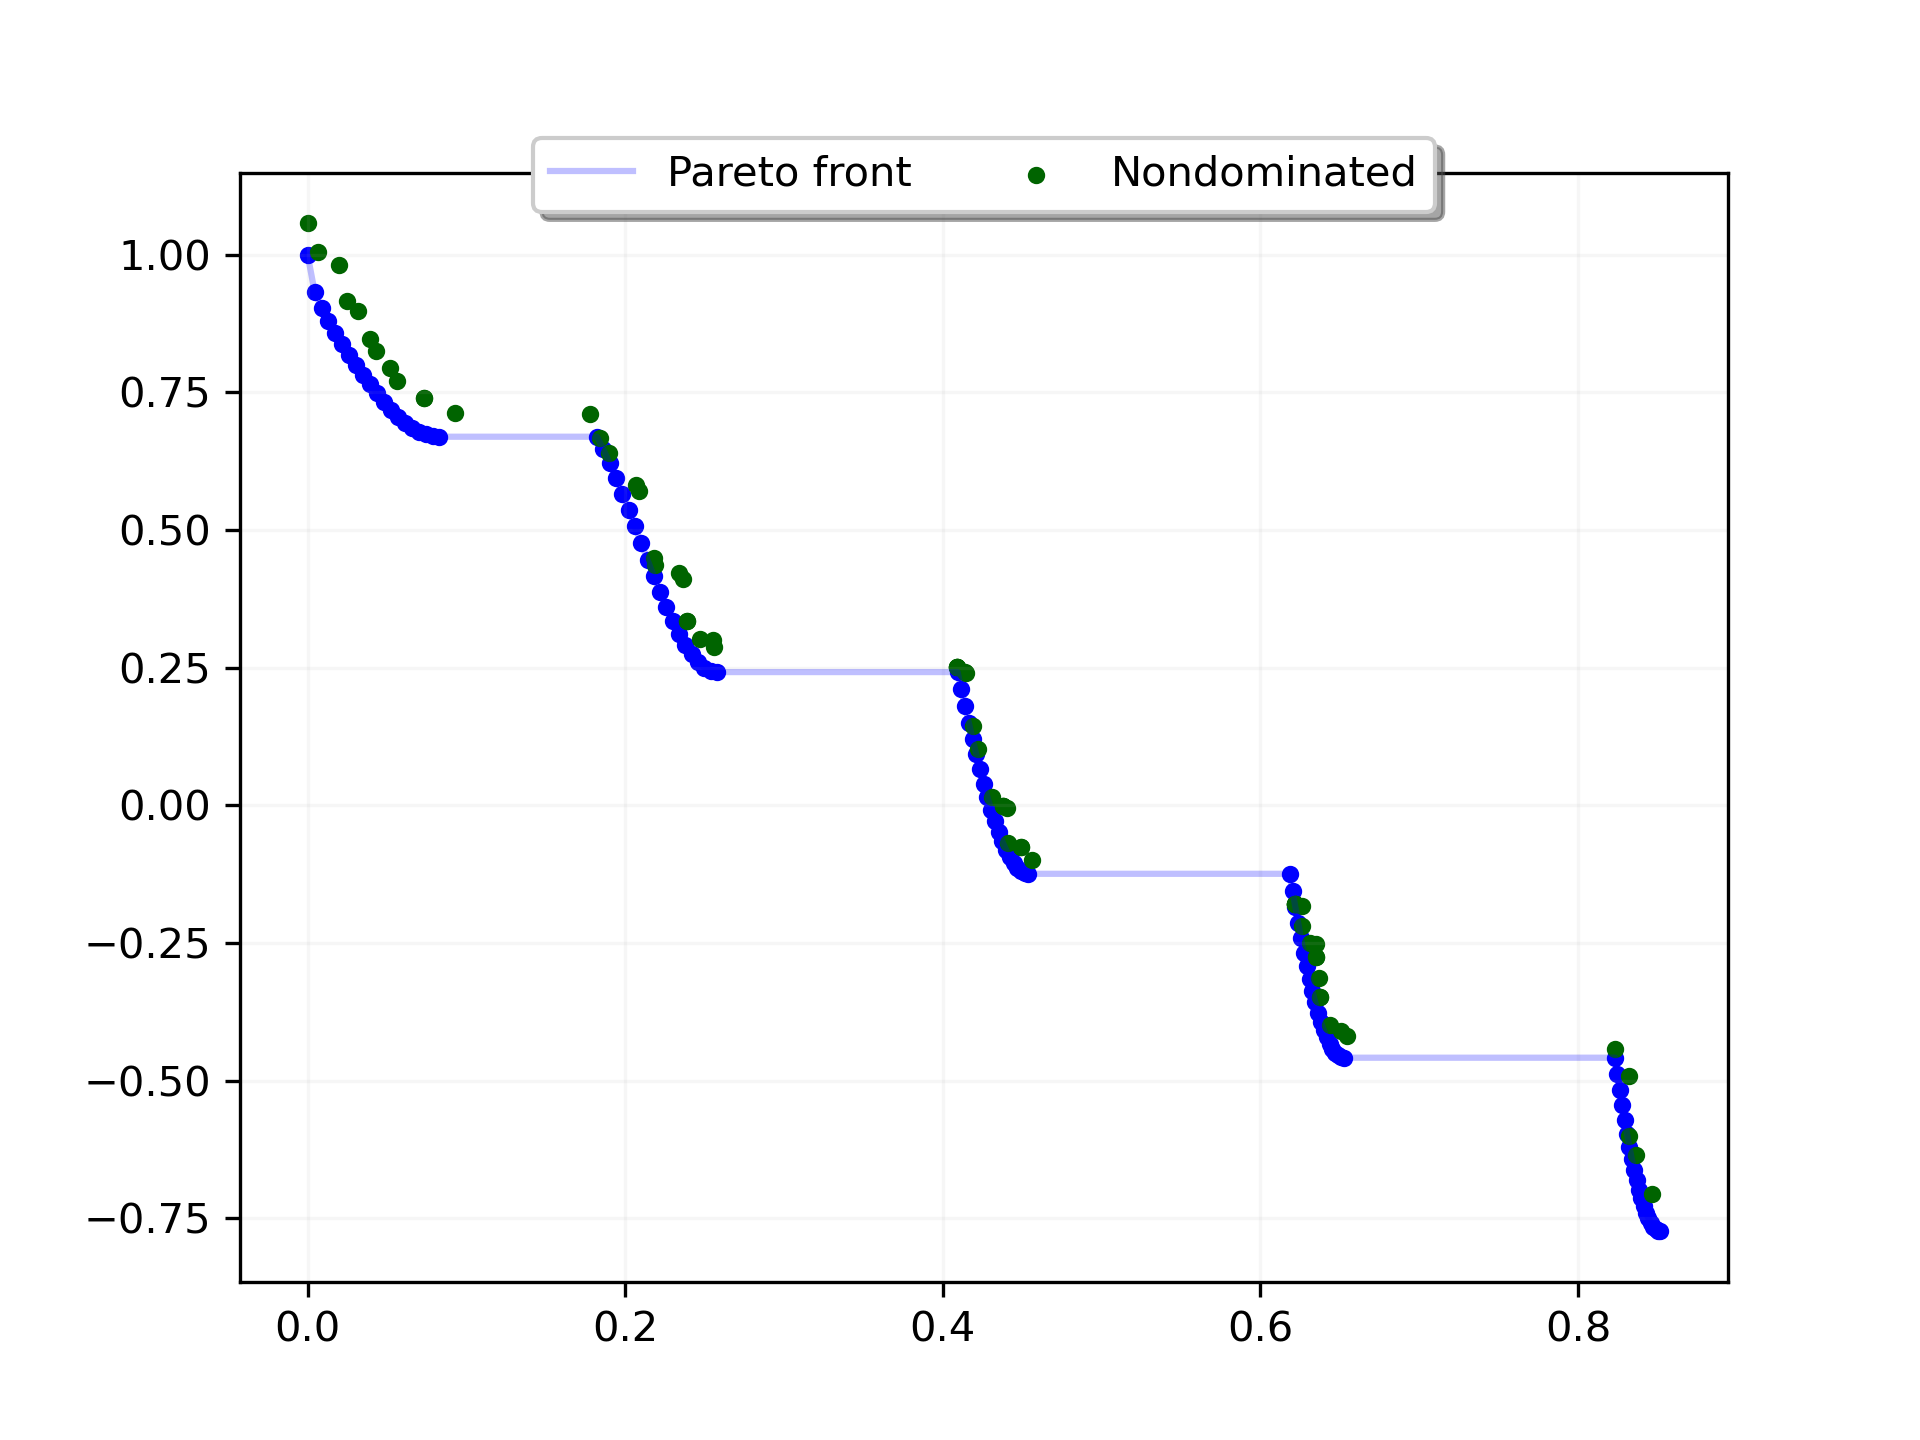
\includegraphics[width=0.9\textwidth]{img2/PESAII_ZDT3_g10000_p50_r0,25.png}
    \caption{Algorytm PESA-II, problem ZDT3, \newline generacje - 10 000, populacja - 50, prawdopodobieństwo - 0,25}
\end{figure}

\begin{figure}[H]
    \centering
    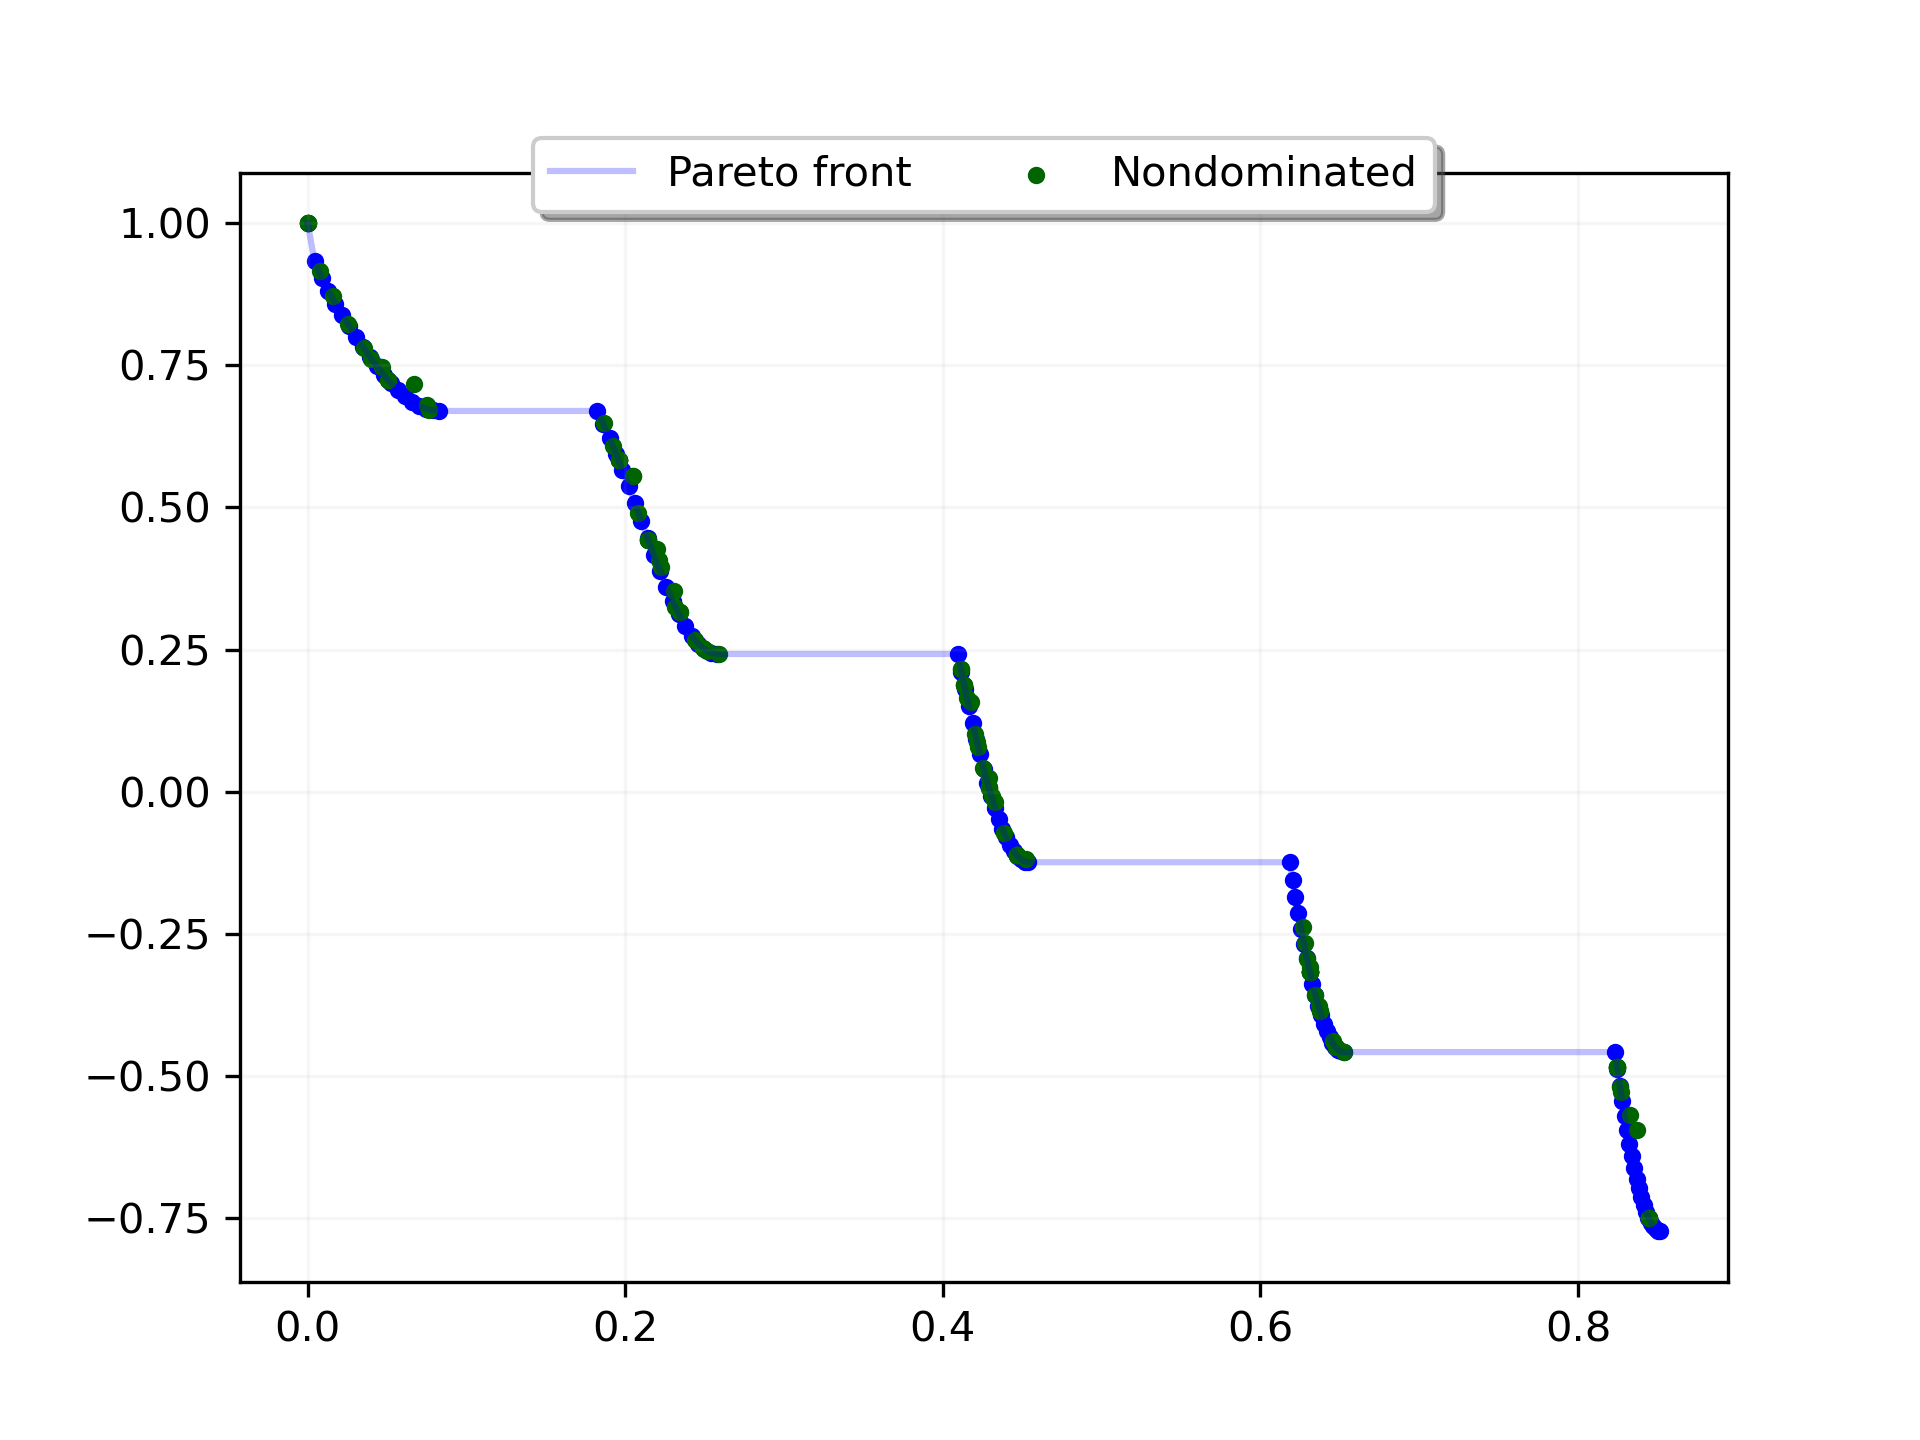
\includegraphics[width=0.9\textwidth]{img2/PESAII_ZDT3_g100000_p200_r0,25.png}
    \caption{Algorytm PESA-II, problem ZDT3, \newline generacje - 100 000, populacja - 200, prawdopodobieństwo - 0,25}
\end{figure}


\subsection{Zmiana parametru divisions}

Sprawdzono czy zmiana parametru divisions (domyślnie jego wartość wynosi 8) wpłynie zauważalnie na rezultaty algorytmu dla ustawień: generacje - 10 000, populacja - 50, prawdopodobieństwo - 0,25.

\begin{table}[H]
\centering
\caption{Wyniki algorytmu PESA-II (generacje - 10 000, populacja - 50, prawdopodobieństwo - 0,25) dla problemu ZDT1}
\label{tab:PESAII_e_ZDT1}
\begin{tabular}{|c|c|c|}
\hline
\textbf{divisions} & \textbf{GD} & \textbf{HV} \\ \hline
4 & 0,016 & 4,636 \\ \hline
\textbf{8} & \textbf{0,015} & \textbf{4,639} \\ \hline
12 & 0,02 & 4,628 \\ \hline
\end{tabular}
\end{table}

\begin{table}[H]
\centering
\caption{Wyniki algorytmu PESA-II (generacje - 10 000, populacja - 50, prawdopodobieństwo - 0,25) dla problemu ZDT2}
\label{tab:PESAII_e_ZDT2}
\begin{tabular}{|c|c|c|}
\hline
\textbf{divisions} & \textbf{GD} & \textbf{HV} \\ \hline
4 & 0,013 & 4,304 \\ \hline
\textbf{8} & \textbf{0,011} & \textbf{4,31} \\ \hline
12 & 0,018 & 4,294 \\ \hline
\end{tabular}
\end{table}

\begin{table}[H]
\centering
\caption{Wyniki algorytmu PESA-II (generacje - 10 000, populacja - 50, prawdopodobieństwo - 0,25) dla problemu ZDT3}
\label{tab:PESAII_e_ZDT3}
\begin{tabular}{|c|c|c|}
\hline
\textbf{divisions} & \textbf{GD} & \textbf{HV} \\ \hline
\textbf{4} & \textbf{0,014} & \textbf{4,998} \\ \hline
\textbf{8} & \textbf{0,013} & \textbf{4,991} \\ \hline
12 & 0,017 & 4,987 \\ \hline
\end{tabular}
\end{table}

\begin{figure}[H]
    \centering
    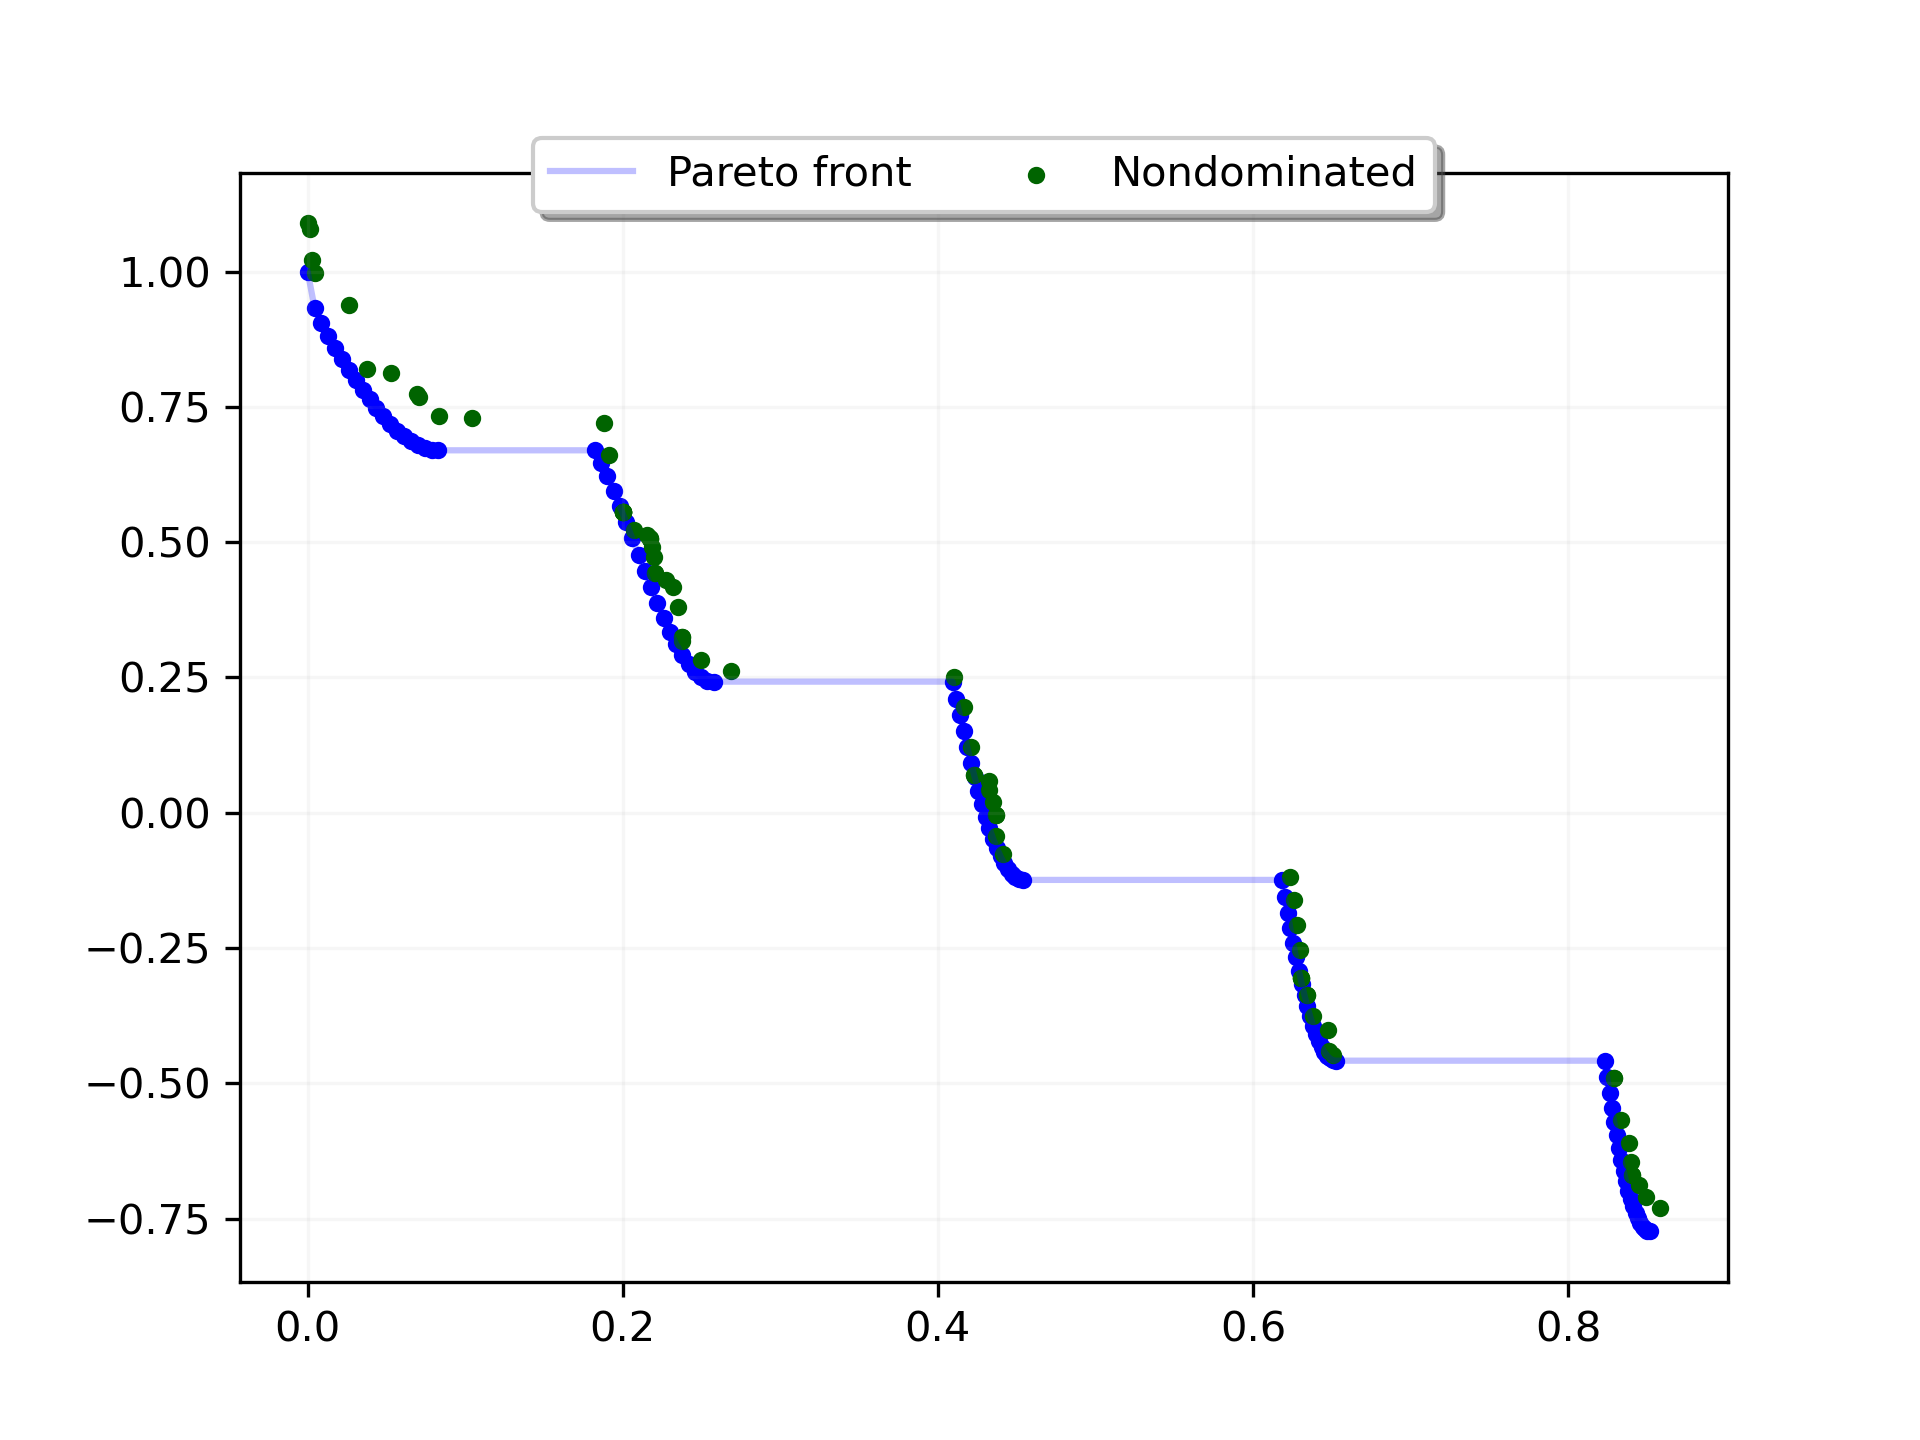
\includegraphics[width=0.9\textwidth]{img2/PESAII_ZDT3_g10000_p50_r0,25_e4.png}
    \caption{Algorytm PESA-II, problem ZDT3, \newline generacje - 100 000, populacja - 50, prawdopodobieństwo - 0,25, divisions - 4}
\end{figure}

%%%%%%%%%%%%%%%%%%%%%%%%%%%%%%%%%%%%%%%%%%%% Wnioski

\section{Wnioski}

\begin{itemize}
    \item Większa liczba generacji pozytywnie wpływa na uzyskanie wyniki optymalizacji, jednocześnie zauważalnie wydłużając czas działania algorytmów. Dla 100 000 generacji rezultaty pokrywały się z frontem Pareto.
    \item Dla niskich wartości generacji, prawdopodobieństwo 0,25 było najgorszym wyborem. Optymalny wybór nie był ściślie powiązany z żadnym algorytmem bądź problemem.
    \item Dla każdego algorytmu oraz dla wysokich wartości generacji (10 000 oraz 100 000) najlepszym prawdopodobieństwem było 0,25.
    \item Wszystkie algorytmy osiągały najlepsze rezultaty dla populacji 50 - dla 100 000 generacji wielkość populacji nie miała znaczenia. Duża populacja przy miarach GD oraz Hypervolume nie wpływa pozytywnie na wyniki.
    \item Średnio, najlepsze wyniki uzyskał algorytm PESA-II, a najgorsze SPEA-II. Dla 100 000 generacji różnice te są pomijalne.
    \item Zmiana parametrów konkretnych argumentów nie wpływa znacząco na rezultaty.

\end{itemize}

\newpage

\nocite{*}
\bibliographystyle{plain-pl}
\bibliography{bib2.bib}

\end{document}

